% !TEX root = main.tex
% \documentclass{tufte-book}%[a4paper,twoside]
% See https://github.com/Tufte-LaTeX/tufte-latex/blob/master/sample-book.tex for details

% --- AMAZON BEGIN ---
% WITHOUT BLEED
% US Trade => 6x9
\documentclass[paper=6in:9in,pagesize=pdftex,
               headinclude=on,footinclude=on,12pt]{scrreprt}
%
% Paper width
% W = 6in
% Paper height
% H = 9in
% Paper gutter
% BCOR = 0.5in
% Margin (0.5in imposed on lulu, recommended on createspace)
% m = 0.5in
% Text height
% h = H - 2m = 8in
% Text width
% w = W - 2m - BCOR = 4.5in
\areaset[0.50in]{4.5in}{8in}
% --- AMAZON END ---

%encoding
%--------------------------------------
\usepackage[T1]{fontenc}
\usepackage[utf8]{inputenc}
%--------------------------------------

%Portuguese-specific commands
%--------------------------------------
\usepackage[brazil]{babel}
%--------------------------------------

% Copyright with title BEGIN
\usepackage{fancyhdr}
\def\secondpage{\clearpage\null\vfill
\pagestyle{empty}
\begin{minipage}[b]{0.9\textwidth}

\normalsize\raggedright
\setlength{\parskip}{0.5\baselineskip}
Obtenha a versão atualizada online em \href{https://inventingbitcoin.com}{inventingbitcoin.com} \par

\footnotesize\raggedright
\setlength{\parskip}{0.5\baselineskip}
Copyright \copyright 2019--\the\year\ Yan Pritzker / \href{https://twitter.com/skwp}{@skwp} / \href{https://yanpritzker.com/}{yanpritzker.com} \par

\footnotesize\raggedright
\setlength{\parskip}{0.5\baselineskip}
Tradução feita por KoreaComK / \href{https://twitter.com/koreacomk}{@KoreacomK} \par

Capa e ilustrações Copyright © 2019 de Nicholas Evans, a menos que haja outra legenda.
\newline
Todos os direitos reservados.
\newline
\footnotesize\raggedright
\setlength{\parskip}{0.5\baselineskip}
Nenhuma parte deste livro pode ser reproduzida em qualquer forma ou por qualquer meio eletrônico ou mecânico, incluindo sistemas de armazenamento e recuperação de informações, sem a permissão por escrito do autor, exceto para o uso de breves citações em uma resenha de livro.

\end{minipage}
\vspace*{2\baselineskip}
\cleardoublepage
\rfoot{\thepage}}

\makeatletter
\g@addto@macro{\maketitle}{\secondpage}
\makeatother
% Copyright with title END

% Use serif font for chapters and parts
\setkomafont{disposition}{\bfseries}
\KOMAoptions{headings=small}

% Packages
\usepackage{setspace}
\usepackage{booktabs}
\usepackage{graphicx}
\setkeys{Gin}{width=\linewidth,totalheight=\textheight,keepaspectratio}
\graphicspath{{graphics/}}

%%
% For Quotes
\usepackage{csquotes}
\renewcommand\mkbegdispquote[2]{\makebox[0pt][r]{\textquotedblleft\,}}
\renewcommand\mkenddispquote[2]{\,\textquotedblright#2}

%%
% Just some sample text
\usepackage{lipsum}

%%
% For nicely typeset tabular material
\usepackage{booktabs}

%%
% Bibliography stuff: Biber, BibTex, BibLatex
%\usepackage[autostyle]{csquotes}
% \usepackage[
    % backend=biber,
    % style=authoryear-icomp,
    % sortlocale=de_DE,
    % natbib=true,
    % url=false,
    % doi=true,
    % eprint=false
% ]{biblatex}
% \usepackage[backend=biber]{biblatex}
\usepackage{url}
\usepackage{natbib}
\bibliographystyle{plain}

%%
% Hyperlinks
\usepackage[hidelinks]{hyperref}


%%
% For graphics / images
\usepackage{caption}
\usepackage{graphicx}
\setkeys{Gin}{width=\linewidth,totalheight=\textheight,keepaspectratio}
\graphicspath{{graphics/}}

% The fancyvrb package lets us customize the formatting of verbatim
% environments.  We use a slightly smaller font.
\usepackage{fancyvrb}
\fvset{fontsize=\normalsize}

%%
% Prints argument within hanging parentheses (i.e., parentheses that take
% up no horizontal space).  Useful in tabular environments.
\newcommand{\hangp}[1]{\makebox[0pt][r]{(}#1\makebox[0pt][l]{)}}

%%
% Prints an asterisk that takes up no horizontal space.
% Useful in tabular environments.
\newcommand{\hangstar}{\makebox[0pt][l]{*}}

%%
% Prints a trailing space in a smart way.
\usepackage{xspace}

% Prints the month name (e.g., January) and the year (e.g., 2008)
\newcommand{\monthyear}{%
  \ifcase\month\or January\or February\or March\or April\or May\or June\or
  July\or August\or September\or October\or November\or
  December\fi\space\number\year
}


% Prints an epigraph and speaker in sans serif, all-caps type.
\newcommand{\openepigraph}[2]{%
  %\sffamily\fontsize{14}{16}\selectfont
  \begin{fullwidth}
  \sffamily\large
  \begin{doublespace}
  \noindent\allcaps{#1}\\% epigraph
  \noindent\allcaps{#2}% author
  \end{doublespace}
  \end{fullwidth}
}
%%%%%%%%%%%%%%%%%%%%%%%%%%%%%%%%%% RAFAEL ADICIONOU ESSA SEçAO PQ FICOU DE SACO CHEIO DE TRADUZIR NOMES E TEM MUITO TEMPO LIVRE
%%%%%%%%%%%%%%%%%%%%%%%%%%%%%%%%%%%%%%%%%%%%%%%%%%%%%%%%%%%%
\newcommand{\TraducaoNomeA}{Ana}
\newcommand{\TraducaoNomeB}{Bruno}
\newcommand{\TraducaoNomeC}{Carol}
\newcommand{\TraducaoNomeH}{Henrique}
\newcommand{\TraducaoNomeZ}{Zelia}

%%%%%%%%%%%%%%%%%%%%%%%%%%%%%%%%%%%%%%%%%%%%%%%%%%%%%%%%%%%%
% Inserts a blank page
\newcommand{\blankpage}{\newpage\hbox{}\thispagestyle{empty}\newpage}

\usepackage{units}

% Typesets the font size, leading, and measure in the form of 10/12x26 pc.
\newcommand{\measure}[3]{#1/#2$\times$\unit[#3]{pc}}

% Macros for typesetting the documentation
\newcommand{\hlred}[1]{\textcolor{Maroon}{#1}}% prints in red
\newcommand{\hangleft}[1]{\makebox[0pt][r]{#1}}
\newcommand{\hairsp}{\hspace{1pt}}% hair space
\newcommand{\hquad}{\hskip0.5em\relax}% half quad space
\newcommand{\TODO}{\textcolor{red}{\bf TODO!}\xspace}
\newcommand{\na}{\quad--}% used in tables for N/A cells
\providecommand{\XeLaTeX}{X\lower.5ex\hbox{\kern-0.15em\reflectbox{E}}\kern-0.1em\LaTeX}
\newcommand{\tXeLaTeX}{\XeLaTeX\index{XeLaTeX@\protect\XeLaTeX}}
% \index{\texttt{\textbackslash xyz}@\hangleft{\texttt{\textbackslash}}\texttt{xyz}}
\newcommand{\tuftebs}{\symbol{'134}}% a backslash in tt type in OT1/T1
\newcommand{\doccmdnoindex}[2][]{\texttt{\tuftebs#2}}% command name -- adds backslash automatically (and doesn't add cmd to the index)
\newcommand{\doccmddef}[2][]{%
  \hlred{\texttt{\tuftebs#2}}\label{cmd:#2}%
  \ifthenelse{\isempty{#1}}%
    {% add the command to the index
      \index{#2 command@\protect\hangleft{\texttt{\tuftebs}}\texttt{#2}}% command name
    }%
    {% add the command and package to the index
      \index{#2 command@\protect\hangleft{\texttt{\tuftebs}}\texttt{#2} (\texttt{#1} package)}% command name
      \index{#1 package@\texttt{#1} package}\index{packages!#1@\texttt{#1}}% package name
    }%
}% command name -- adds backslash automatically
\newcommand{\doccmd}[2][]{%
  \texttt{\tuftebs#2}%
  \ifthenelse{\isempty{#1}}%
    {% add the command to the index
      \index{#2 command@\protect\hangleft{\texttt{\tuftebs}}\texttt{#2}}% command name
    }%
    {% add the command and package to the index
      \index{#2 command@\protect\hangleft{\texttt{\tuftebs}}\texttt{#2} (\texttt{#1} package)}% command name
      \index{#1 package@\texttt{#1} package}\index{packages!#1@\texttt{#1}}% package name
    }%
}% command name -- adds backslash automatically
\newcommand{\docopt}[1]{\ensuremath{\langle}\textrm{\textit{#1}}\ensuremath{\rangle}}% optional command argument
\newcommand{\docarg}[1]{\textrm{\textit{#1}}}% (required) command argument
\newenvironment{docspec}{\begin{quotation}\begin{samepage}\ttfamily\parskip0pt\parindent0pt\ignorespaces}{\end{flushright}\end{samepage}\end{quotation}}% command specification environment
\newcommand{\docenv}[1]{\texttt{#1}\index{#1 environment@\texttt{#1} environment}\index{environments!#1@\texttt{#1}}}% environment name
\newcommand{\docenvdef}[1]{\hlred{\texttt{#1}}\label{env:#1}\index{#1 environment@\texttt{#1} environment}\index{environments!#1@\texttt{#1}}}% environment name
\newcommand{\docpkg}[1]{\texttt{#1}\index{#1 package@\texttt{#1} package}\index{packages!#1@\texttt{#1}}}% package name
\newcommand{\doccls}[1]{\texttt{#1}}% document class name
\newcommand{\docclsopt}[1]{\texttt{#1}\index{#1 class option@\texttt{#1} class option}\index{class options!#1@\texttt{#1}}}% document class option name
\newcommand{\docclsoptdef}[1]{\hlred{\texttt{#1}}\label{clsopt:#1}\index{#1 class option@\texttt{#1} class option}\index{class options!#1@\texttt{#1}}}% document class option name defined
\newcommand{\docmsg}[2]{\bigskip\begin{fullwidth}\noindent\ttfamily#1\end{fullwidth}\medskip\par\noindent#2}
\newcommand{\docfilehook}[2]{\texttt{#1}\index{file hooks!#2}\index{#1@\texttt{#1}}}
\newcommand{\doccounter}[1]{\texttt{#1}\index{#1 counter@\texttt{#1} counter}}

% Generates the index
\usepackage{makeidx}
\makeindex

%%
% Chapter/Lesson Quotes
\makeatletter
\renewcommand{\@chapapp}{}% Not necessary...
\newenvironment{chapquote}[2][4em]
  {\setlength{\@tempdima}{#1}%
   \def\chapquote@author{#2}%
   \parshape 1 \@tempdima \dimexpr\textwidth-2\@tempdima\relax%
   \itshape}
  {\par\normalfont\hfill--\ \chapquote@author\hspace*{\@tempdima}\par\bigskip}
  
\usepackage{amsmath}

\usepackage[tocindentauto]{tocstyle}
\usetocstyle{KOMAlike} %the previous line resets it
%%%%%%%%%%%%%%%%%%%%%%%%%%%%%%%%%%%%%%%%%%%%%%%%%%%%%%%%%%%%%%%%%%%%%%%%%%%%%%%%
%                                   DOCUMENT
%%%%%%%%%%%%%%%%%%%%%%%%%%%%%%%%%%%%%%%%%%%%%%%%%%%%%%%%%%%%%%%%%%%%%%%%%%%%%%%%

\begin{document}

%\frontmatter
\pagenumbering{roman}

\title{Inventando o Bitcoin}
\subtitle{Explicando a tecnologia por trás do primeiro dinheiro verdadeiramente escasso e descentralizado}
\author{Yan Pritzker}
\date{}

\maketitle
\cleardoublepage

\newpage \vspace*{8cm}
\thispagestyle{empty}
\begin{quotation}
\begin{center}
  \large
  \enquote{Este livro é dedicado a meus pais Yury e Lana, que tiraram nossa família da ex-URSS, um regime socialista autocrático com rígidos controles de capital}.
\end{center}
\end{quotation}
\begin{quotation}
\begin{center}
  \enquote{Também é dedicado à minha esposa Jessica, que teve que suportar minha incapacidade de parar de falar sobre o Bitcoin, e por ficar acordada comigo até tarde para terminar este livro}.
\end{center}
\end{quotation}

\renewcommand{\baselinestretch}{0.50}\normalsize
\tableofcontents
\renewcommand{\baselinestretch}{1.0}\normalsize

%%
% Start the main matter (normal chapters)
%\mainmatter
\pagenumbering{arabic}

\chapter*{Introdução}
\label{ch:introducao}

Bem-vindo ao \textit{Inventando o Bitcoin!}

Meu objetivo é simplesmente agradar seu cérebro e dar a você um gostinho da ciência da computação e da teoria dos jogos econômicos que fazem do Bitcoin uma das invenções mais interessantes e profundas de nosso tempo.

A maioria das pessoas, ao ouvir pela primeira vez sobre o Bitcoin, realmente não o entendem. É dinheiro mágico da internet? De onde isso vem? Quem o controla? Por que é tão importante?

Para mim, entender todas as coisas que se juntam para fazer o Bitcoin funcionar - física, matemática, criptografia, teoria dos jogos, economia e ciência da computação - foi um momento profundo. Neste livro, espero compartilhar esse conhecimento com você de uma forma muito simples e fácil de entender.

A forma como o faremos isso é um passo de cada vez. Com nada além de uma base de matemática de nível médio, iremos percorrer a \textit{invenção do bitcoin}, passo a passo. Espero que este livro seja o suficiente para dar um gostinho do que é essa tecnologia e mandá-lo para o buraco do coelho do Bitcoin. Então, vamos começar!
\chapter{O que é o Bitcoin?}
\label{ch:capitulo1}
%\section**{O que é o Bitcoin?}

O Bitcoin é um \textit{dinheiro eletrônico ponto a ponto}. Um dinheiro digital que pode ser transferido entre pessoas ou computadores sem nenhum intermediário confiável (como um banco) e cuja emissão não está sob o controle de nenhuma parte.

Pense em uma nota de dois reais ou em uma moeda de metal. Quando você dá esse dinheiro para outra pessoa, ela não precisa saber quem você é. Eles só precisam confiar que o dinheiro que recebem de você não é uma falsificação. Tipicamente, as pessoas fazem isso com dinheiro físico, usando apenas os olhos e os dedos, ou ate em casos de quantias maiores usando equipamentos próprios para testar cédulas.

Conforme mudamos para uma sociedade digital, pagamentos começaram a ser feitos digitalmente pela internet por meio de um serviço de intermediário, do que fisicamente: uma empresa de cartão de crédito como Visa, um provedor de pagamento digital como PayPal ou Apple Pay ou um serviço online de uma plataforma, como o WeChat na China.

A mudança para pagamentos digitais traz consigo a dependência em uma entidade central que tem que aprovar e verificar cada pagamento. Isso ocorre porque a natureza do dinheiro mudou de uma coisa física que você pode carregar trocar e verificar por si mesmo, para bits digitais que precisam ser verificados pela parte que controla sua transferência.


Ao trocarmos nosso dinheiro físico por pagamentos digitais, nos também criamos um sistemas onde damos poderes extraordinários a aqueles que buscam nos oprimir.
Plataformas de pagamentos digitais se tornaram a base de um futuro sistema autoritário distópico, tal qual aqueles utilizados pelo governo chines para monitorar seus dissentes e prevenir cidadãos, cujo seu comportamento não estão ao seu agrado, de comprar bens e serviços.

O Bitcoin oferece uma alternativa ao dinheiro digital controlado centralmente com um sistema de três componentes básicos. Veremos as motivações por trás desse design na próxima seção.

\begin{samepage}
\begin{enumerate}
\item Um ativo digital (normalmente \textit{bitcoin} com \textit{b} minúsculo) com um suprimento que é limitado, conhecido com antecedência e imutável. Isso contrasta fortemente com o dinheiro com o qual a maioria de nós está acostumado atualmente, que são notas emitidas por governos ou bancos centrais cuja oferta se expande a uma taxa imprevisível, com o passar do tempo.
\item Um monte de computadores interconectados (a \textit{rede Bitcoin}, com \textit{B} maiúsculo), aos quais qualquer pessoa pode entrar. Essa rede serve para rastrear a propriedade de bitcoins e transferi-los entre os participantes, evitando qualquer intermediário, como bancos, empresas de pagamento e entidades governamentais.
\item O software Bitcoin Client, que é um pedaço de código que qualquer pessoa pode executar em seu computador para se tornar um participante da rede. Este software é de código aberto, o que significa que qualquer pessoa pode ver como funciona, bem como contribuir com novos recursos e correções de bugs.
\end{enumerate}
\end{samepage}

%\newpage

\begin{figure}
  \centering
  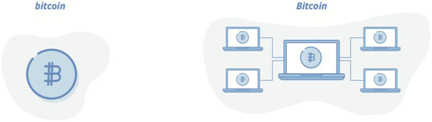
\includegraphics[width=10cm]{imagens/bitcoin-capitulo-1.png}
  \caption*{\textit{\small bitcoin e Bitcoin}}
\end{figure}
  
%\newpage
\section*{De onde veio o Bitcoin?}
%\paragraph{}

O Bitcoin foi inventado por uma pessoa ou grupo de pessoas, conhecido pelo pseudônimo de Satoshi Nakamoto, por volta de 2008. Ninguém sabe a identidade dessa(s) pessoa(s) e, pelo que sabemos, sumiram, não se houve falar dele(s) há anos.

Em 11 de fevereiro de 2009, Satoshi revelou o primeiro protótipo do Bitcoin em um fórum online para os cypherpunks, pessoas que trabalham com tecnologia de criptografia e se preocupam com a privacidade individual.
Embora essa não é o primeiro  anuncio do Bitcoin, contem uma bom sumario das motivações de Satoshi, a usaremos para fundamentar nossa discussão

Extraí as partes relevantes abaixo. Na próxima seção, explicaremos algumas dessas declarações e as motivações de Satoshi para a invenção do Bitcoin e quais problemas ele buscava solucionar.

\begin{quotation}\begin{samepage}
\enquote{\textit{
Desenvolvi um novo sistema de e-cash P2P de código aberto chamado Bitcoin. É totalmente descentralizado, sem servidor central ou partes confiáveis, porque tudo é baseado em criptografia ao invés da confiança. [\ldots]}

\textit{A raiz do problema com a moeda convencional é toda a confiança necessária para fazê-la funcionar. O banco central deve ser confiável para não depreciar a moeda, mas a história das moedas fiduciárias está cheia de violações dessa confiança. Os bancos devem ser confiáveis para manter nosso dinheiro e transferi-lo eletronicamente, mas eles o emprestam em ondas de bolhas de crédito ficando apenas com uma fração na reserva. Temos que confiar neles à nossa privacidade, confiar que não irão permitir que ladrões de identidade drenem nossas contas. Seus enormes custos indiretos tornam os micro pagamentos impossíveis.}

\textit{Na geração passada, os sistemas de compartilhamento de tempo multiusuário tinham um problema semelhante. Antes da criptografia forte, os usuários tinham que confiar na proteção por senha para proteger seus arquivos[\ldots]}

\textit{Então, a criptografia forte tornou-se disponível para as massas e a confiança não era mais necessária. Os dados podiam ser protegidos de uma forma fisicamente impossível para outras pessoas acessarem, não importa por que razão, não importa quão boa seja a desculpa, não importa o quê seja criptografado.}
 
\textit{É hora de termos o mesmo no nosso dinheiro. Com a moeda eletrônica baseada em prova criptográfica, sem a necessidade de confiar em um intermediário, o dinheiro pode ser seguro e as transações com o mínimo de esforço.[\ldots]}
 
\textit{A solução do Bitcoin é usar uma rede ponto a ponto para verificar se há gastos duplos. Em suma, a rede funciona como um servidor de carimbo de data/hora distribuído, carimbando a primeira transação a gastar uma moeda. Ele tira proveito da natureza da informação ser fácil de ser espalhada, mas difícil de ser reprimida. Para obter detalhes sobre seu funcionamento, consulte o design desta solução no artigo disponibilizado em
\newline \textcolor{red}{http://www.bitcoin.org/bitcoin.pdf}}}
\begin{flushright} -- Satoshi Nakamoto
\end{flushright}\end{samepage}\end{quotation}

Quando o Bitcoin foi lançado, apenas algumas pessoas o utilizavam e executavam seu sistema em seus computadores (chamados de \textit{nodes}) para alimentar a rede Bitcoin. A maioria das pessoas na época achou que era uma piada ou que o sistema revelaria sérias falhas no projeto, que o tornaria impraticável.

Com o tempo, mais pessoas se juntaram à rede, usando seus computadores para adicionar segurança à ela e reforçando seu valor, trocando outras moedas pelo Bitcoin ou aceitando-a por bens e serviços. Hoje, dez anos depois, é usado por milhões de pessoas com dezenas a centenas de milhares de nodes executando o software gratuito do Bitcoin, que é desenvolvido por centenas de voluntários e empresas em todo o mundo.

O Bitcoin não foi uma invenção criada do nada. Em seu artigo, Satoshi citou várias tentativas importantes de implementar sistemas semelhantes, incluindo o b-money de Wei Dai e o Hashcash de Adam Back. A invenção do Bitcoin apoiou-se nos ombros de gigantes e, no entanto, foi profunda em sua simplicidade ao criar o primeiro sistema verdadeiramente descentralizado - isto é, que não está sob controle de uma pessoa - para emitir e transferir dinheiro digital.

%\newpage
\section*{O Bitcoin resolve quais problemas?}
%\paragraph{}
 
Vamos detalhar algumas das postagens do Satoshi. Ao longo do livro, abordaremos como esses conceitos são realmente implementados. Não é importante que você entenda imediatamente todos os conceitos difíceis desta seção, mas você vai querer ver quais eram os objetivos do Satoshi, para que possamos almejá-los à medida que avançamos no exercício de \textit{Inventar o Bitcoin}.


\paragraph{}
\textit{Desenvolvi um novo sistema de e-cash P2P de código aberto}
\paragraph{}

O P2P significa ponto a ponto (\textit{peer-to-peer}, no inglês) e indica um sistema onde uma pessoa pode interagir com outra sem intermediários, como sendo pares iguais. Você deve se lembrar das tecnologias de compartilhamento de arquivos P2P, como Napster, Kazaa e BitTorrent, que permitiam que as pessoas compartilhassem música sem baixá-las de um site. O Satoshi projetou o Bitcoin para permitir que as pessoas troquem \textit{e-cash}, dinheiro eletrônico, sem passar por um intermediário da mesma maneira.

O software é de \textit{código aberto}, o que significa que qualquer pessoa pode ver como funciona e contribuir para o projeto. Isso é importante porque elimina a exigência de confiança no próprio Satoshi. Não precisamos acreditar em nada que o Satoshi escreveu em sua postagem sobre como o software funciona. Podemos olhar o código e verificar como ele funciona nós mesmos. Melhor ainda, se não gostarmos de algo, podemos mudar.

\paragraph{}
\textit{É totalmente descentralizado, sem servidor central ou partes confiáveis[\ldots]}
\paragraph{}

Satoshi menciona que o sistema é \textit{descentralizado} para diferenciá-lo de sistemas que possuem controle central. As tentativas anteriores de criar um dinheiro digital como o DigiCash de David Chaum de 1989, eram apoiadas por um \textit{servidor central}, um computador ou conjunto de computadores que era responsável pela emissão e verificação de pagamento, administrado por uma empresa.

Esses esquemas de emissão de dinheiro privado, controlados por uma entidade central, estavam fadados ao fracasso. As pessoas não podem contar com um dinheiro que pode ir embora quando a empresa fecha as portas, é hackeada, sofre uma falha no servidor ou, é fechada pelo governo.

A natureza descentralizada do Bitcoin traz de volta o conceito de dinheiro para o mundo digital: você pode transferi-lo sem falar com ninguém, sem pedir permissão, 24 horas por dia, 365 dias por ano, sem passar por nenhuma autoridade que exige confiança.

\paragraph{}
\textit{\dots tudo é baseado em criptografia ao invés de confiança}
\paragraph{}

A internet e a maioria dos sistemas de computadores modernos são construídos em torno de criptografia, um método de obscurecer informação de tal maneira que apenas o receptor da informação possa decodificar ela.
Como o Bitcoin se livra da exigência de \textit{confiança}? Vamos nos aprofundar neste assunto nos próximos capítulos do livro, mas a ideia básica é que em vez de confiar em alguém que diz "Eu sou Ana" ou "Eu tenho R\$10,00 em minha conta bancária", que significaria acreditar em sua palavra, podemos usar a criptografia matemática para declarar os mesmos fatos de uma forma que seja facilmente verificada pelo destinatário e impossível de ser forjada.
Bitcoin usa criptografia matemática ao longo de todo seu projeto para permitir que participantes possam verificar o comportamento dos mesmos sem confiar em terceiros.
Isso se tornaria a base do sistema do Bitcoin para provar a propriedade dos saldos, bem como fornecer segurança para a rede.

\paragraph{}
\textit{Temos que confiar [nos bancos] nossa privacidade, confiar que não irão permitir que ladrões de identidade drenem nossas contas.}
\paragraph{}

Ao contrário de usar sua conta bancária, sistema de pagamento digital ou cartão de crédito, o Bitcoin permite que duas partes façam transações sem fornecer nenhuma informação de identificação pessoal.

Os repositórios centralizados de dados de consumidores armazenados em bancos, empresas de cartão de crédito, processadores de pagamentos e governos são chamarizes gigantescos para os hackers. Quase que para provar o ponto de Satoshi, a Equifax, foi imensamente comprometida em 2017, quando hackers conseguiram vazar as identidades e dados financeiros de mais de 140 milhões de pessoas.

O Bitcoin separa as transações financeiras das identidades do mundo real. Afinal, quando damos dinheiro físico a alguém, ela não precisa saber quem somos, nem precisamos nos preocupar se, após essa troca, ela poderá usar algumas informações que demos para roubar o nosso dinheiro. Por que não devemos esperar o mesmo, ou coisa pior, quando usamos o dinheiro digital?

\paragraph{}
\textit{O banco central deve ser confiável para não depreciar a moeda, mas a história das moedas fiduciárias está cheia de violações dessa confiança.}
\paragraph{}

\textit{Fiat}, que em latim, significa “que seja feito”, refere-se à moeda emitida pelo governo e pelo banco central que é decretada como curso legal pelo governo. Historicamente, o dinheiro era escolhido livremente pelos participantes do mercado entre coisas difíceis de serem produzidas, fáceis de serem verificadas e transportadas, como sal, conchas, pedras, prata e ouro.
Toda vez que 'algo' era utilizado como dinheiro havia a tentação de criar mais dele. Se alguém viesse com tecnologia superior para rapidamente criar muitos de 'algo', esse 'algo' perdia valor. Era assim que Colonizadores europeus foram capazes de despir o continente africano de suas riquezas, trocando petecas de vidros, facilmente produzidos, por escravos humanos, dificilmente produzidos. Por isso que ouro foi considerado dinheiro por tanto tempo, era difícil de produzir mais dele rapidamente.

Lentamente, mudamos para uma economia mundial que usava o ouro como dinheiro para uma em que o papel passou a representar uma reivindicação desse metal precioso. Eventualmente, o papel foi totalmente separado de qualquer respaldo físico com o pronunciamento do presidente Nixon, que acabou com a conversibilidade internacional do dólar americano em ouro em 1971. 

O fim deste padrão permitiu que governos e bancos centrais aumentassem a oferta de dinheiro à vontade, diluindo o valor de cada nota em circulação, conhecida como \textit{depreciação}. Embora apoiada pelo governo e impossível de ser resgatável por algo palpável, a moeda puramente fiduciária é o dinheiro que todos conhecemos e usamos no dia a dia, na verdade é um conceito relativamente novo, com menos de um século de vida.

Confiamos que nossos governos não abusarão de suas impressoras, mas não precisamos ir muito longe na história em busca de exemplos de \textit{violação dessa confiança}. Em regimes autocráticos e de planejamento central, em que o governo tem a posse direta da máquina de impressão de dinheiro, como a Venezuela, a moeda perdeu quase todo o seu valor. O bolívar venezuelano passou de 2 bolívar por dólar em 2009 para 250.000 bolívar por dólar em 2019. No momento em que escrevo este livro, a Venezuela está em processo de colapso devido à terrível má gestão de sua economia por seu governo.

Em contraste com a moeda \textit{fiduciária} emitida centralmente, cuja oferta não pode ser prevista, a fim de evitar a \textit{depreciação}, Satoshi projetou um sistema de dinheiro em que a oferta era fixa e emitida a uma taxa previsível e imutável. Haverá apenas 21 milhões de bitcoins, embora cada um possa ser dividido em 100 milhões de unidades, chamadas de satoshis, produzindo um total de 2.1 quadrilhões de satoshis em circulação ate o ano de 2140.

Antes do Bitcoin, os ativos digitais não eram escassos. É fácil copiar um livro digital, arquivo de áudio ou vídeo e enviá-lo a um amigo. As únicas exceções são os ativos digitais controlados por intermediários. Por exemplo, ao alugar um filme no iTunes, você pode assisti-lo em seu dispositivo apenas porque o iTunes controla a entrega do filme e pode interrompê-lo após o término do período de locação. Da mesma forma, seu dinheiro digital é controlado pelo seu banco. É função do banco manter um registro de quanto dinheiro você possui e, se você transferi-lo para outra pessoa, ele pode autorizar ou negar essa transferência.

O Bitcoin é a primeira rede digital que impõe escassez sem intermediários e é o primeiro ativo conhecido pela humanidade cujo fornecimento inalterável e cronograma de emissão são conhecidos com antecedência. Nem mesmo metais preciosos como o ouro têm essa propriedade, uma vez que sempre podemos minerar mais e mais depósitos de ouro a uma taxa imprevisível, se for lucrativo fazê-lo. 
Imagina encontrar um asteroide contendo dez vezes mais ouro que nossas reservas no planeta, o que aconteceria com o preço do ouro dado uma oferta tão abundante.
Bitcoin é imune a tais descobertas e manipulações de demanda. É simplesmente impossível de produzir mais dele.
Veremos como isso é aplicado nos próximos capítulos.

A natureza da dinheiro e o funcionamento do sistema monetário atual são intrínsecos, e neste livro não serão detalhados em profundidade adequada. Caso queiras aprender mais sobre tais fundamentos do dinheiro e como eles se aplicam ao Bitcoin recomendo a leitura do livro \textit{O Padrão Bitcoin} por Saifedean Ammous, como ponto de partida

\paragraph{}
\textit{Os dados podiam ser protegidos de uma forma fisicamente impossível para outras pessoas acessarem, não importando o motivo, quão boa a desculpa, não importando nada[\ldots] É hora de termos o mesmo no nosso dinheiro.}
\paragraph{}

Nossos sistemas atuais de proteção de dinheiro, como quando fazemos um depósito em um banco, dependem de confiar em outra pessoa para fazer o trabalho. Confiar em tal intermediário não requer apenas confiança de que eles não farão algo malicioso ou tolo, e que os hackers não irão roubá-lo, mas também que o governo não confiscará ou congelará os fundos. No entanto, foi demonstrado em todo o mundo, repetidamente, que os governos podem e suprimem o acesso ao dinheiro quando se sentem ameaçados.

Pode parecer bobagem para alguém que mora nos Estados Unidos, ou em outra economia altamente regulamentada, pensar em acordar e ter seu dinheiro confiscado. Ocorreu algo parecido comigo, quando tive meus fundos congelados pelo PayPal simplesmente porque não usava minha conta há meses. Levei mais de uma semana para recuperar o acesso ao “meu” dinheiro. Tenho sorte de morar nos Estados Unidos, um dos poucos países onde pelo menos poderia esperar obter algum alívio legal se o PayPal congelasse meus fundos, e onde tenho a confiança básica de que meu governo e meu banco não roubarão meu dinheiro.

Coisas muito piores aconteceram e estão acontecendo atualmente em países com menos liberdade, como bancos sendo fechados durante colapsos da moeda na Grécia, bancos em Chipre usando depósitos para roubar fundos de seus clientes ou o governo declarando certas notas como sendo sem valor de um dia para o outro, como na Índia, privando as pessoas de sua riqueza, causando corridas em caixas eletrônicos e pessoas morrendo de fome devido à incapacidade de acessar seu capital.

A antiga URSS, onde cresci, tinha uma economia fortemente controlada de modo centralizado, levando a uma escassez massiva de bens. Quando queríamos sair, só podíamos trocar uma quantia limitada de dinheiro por pessoa sob uma taxa de câmbio oficial, controlada pelo governo, que era amplamente desconectada da verdadeira taxa de livre mercado. Efetivamente assim o governou tirou de nos a pouca riqueza q tínhamos através de um controle rígido da economia e movimentos de capitais.

Quando as economias começam a falhar em países autocráticos, elas tendem a implementar controles econômicos rígidos, impedindo as pessoas de sacar seu dinheiro dos bancos, carregá-lo para fora do país ou trocá-lo por moedas que ainda possuem valor, como o dólar americano no livre mercado.
Isso da carta branca ao governo para implementar experimentos econômicos insanos como por exemplo o sistema socialista da URSS.

O Bitcoin fornece um sistema de segurança que não depende da confiança de terceiros para proteger o seu dinheiro. Em vez disso, o Bitcoin torna suas moedas \textit{impossíveis de serem acessadas por outros} sem uma chave especial que só você possui, \textit{não importa por que razão, não importa quão boa seja a desculpa, não importa o quê façam}. Possuindo Bitcoin, você possui a chave para sua liberdade financeira. Bitcoin separa dinheiro do estado.

%O Bitcoin separa o dinheiro do estado e, portanto, fornece um controle sobre autocratas e ditadores, restaurando a liberdade do controle da riqueza e a de transportá-la através das fronteiras sem nenhuma interferência.

\paragraph{}
\textit{A solução do Bitcoin é usar uma rede ponto a ponto para verificar se há gastos duplos[\ldots] como um servidor de carimbo de data/hora distribuído, carimbando a primeira transação para gastar uma moeda.}
\paragraph{}

Uma rede simplesmente se refere à ideia de que vários computadores estão conectados e podem enviar mensagens uns aos outros. A palavra distribuído significa que não há uma entidade central controladora, mas que todos os participantes se coordenam para tornar a rede bem-sucedida.

Em um sistema sem controle central, é importante saber que ninguém está trapaceando. A ideia de \textit{gasto duplo} refere-se à capacidade de gastar o mesmo dinheiro duas vezes. Isso não é um problema com dinheiro físico pois ele sai da sua mão quando o utiliza. Entretanto, transições digitais podem ser copiadas, de maneira similar a musicas ou filmes. Quando movimentas dinheiro através de um banco, o banco garante que o dinheiro não sera movido duas vezes. Em um sistema sem entidade central é necessário encontrar uma maneira de impedir o gasto duplo que na pratica é a mesma coisa que forjar dinheiro.

Satoshi está descrevendo que os participantes da rede Bitcoin trabalham juntos para \textit{marcar o tempo} (colocar em ordem) as transações para que saibamos o que aconteceu primeiro, a fim de evitar que seja possível forjar o dinheiro de maneira digital. Nos próximos capítulos, construiremos esse sistema do zero. Isso nos permitirá detectar falsificações sem depender de nenhum emissor central ou validador de transações.

Bitoin não foi uma invenção do dia para a noite, em seu artigo Satoshi cita diversas tentativas importantes de implementar sistemas similares ao Bitcoin, incluindo o b-money do Wei Dai e o Hashcash do Adam Back. A invenção do Bitcoin foi realizada sobre os ombros de gigantes, mas ninguém ate então havia juntado todas as peças corretas, criando o então primeiro sistemas de criação e transferência de dinheiro digital verdadeiramente escasso, sem a necessidade de um controle central. 

A invenção do Bitcoin resolveu uma série de problemas técnicos interessantes relacionados a privacidade, degradação e controle central nos sistemas monetários atuais. Alguns deles são:

\begin{enumerate}
\item Como criar uma rede ponto a ponto na qual qualquer pessoa pode ingressar e participar voluntariamente;
\item Como um grupo de pessoas que não precisam revelar suas identidades ou confiar umas nas outras pode manter uma contabilidade compartilhada de valores, mesmo que algumas delas sejam desonestas;
\item Como criar uma verdadeira escassez digital sem um intermediário;
\item Como criar um ativo digital que não seja forjável e seja verificável instantaneamente e resistente a roubo e hacking.
\end{enumerate}

Quando Bitcoin foi lançado apenas um punhado de pessoas utilizavam e rodavam um \textit{node} do software Bitcoin nos seus computadores para alimentar a rede Bitcoin. A grande maioria das pessoas da época pensavam que era uma piada, ou que o sistema iria apresentar serias falhas de projeto que o fariam não funcional. 

Com a passagem do tempo mais pessoas se juntaram a rede, utilizando seus computadores a rede se tornou mais segura e reforçando que rede tinha valor ao trocar outras moedas por ela, ou bens e serviços. Hoje dez anos depois a rede é utilizada por milhões de pessoas com dezenas a centenas de milhares de \textit{nodes} rodando o software gratuito do Bitcoin, que foi desenvolvido por centenas de voluntários e empresas ao redor do mundo.

Vamos descobrir como podemos construir este sistema!
\part{Removendo o intermediário}
\label{ch:capitulo2}
\chapter*{Removendo o intermediário}

No capítulo anterior, comentamos que o Bitcoin fornece um sistema ponto a ponto para a transferência de valor. Antes de nos aprofundarmos em como isso funciona, vamos primeiro entender como um banco tradicional ou empresa de pagamento lida com o rastreamento da propriedade e das transferências de ativos.

\paragraph{Os bancos são apenas livros contábeis}
\paragraph{}

Como funciona um pagamento digital feito por seu banco, PayPal ou ApplePay? Muito simples, essas entidades intermediárias têm um livro-razão de contas e transferências.

Neste exemplo, vamos utilizar a expressão \textit{banco}, mas realmente queremos dizer qualquer outra entidade que processa pagamentos. Começamos com um livro-razão de contas que mostra que Ana e Bruno depositaram dinheiro no banco.

\newpage
\begin{figure}
  \centering
  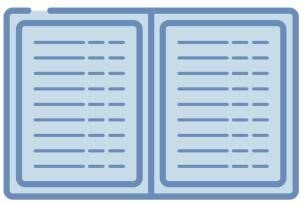
\includegraphics[width=4cm]{imagens/livro-capitulo-02.jpg}  
  \caption{Livro-razão}
\end{figure}

\paragraph{}
\textbf{Livro razão do banco}

\begin{samepage}
\begin{enumerate}
\item Ana: Crédito por depósito em dinheiro +R\$2,00
\item Bruno: Crédito por depósito em dinheiro +R\$10,00
\end{enumerate}
\end{samepage}

Quando Ana deseja enviar R\$2,00 para Bruno, ela liga para seu banco ou usa o \textit{internet banking} ou um aplicativo disponibilizado pela empresa, autentica-se usando um nome de usuário e senha ou um código PIN e, em seguida, faz a solicitação de transferência. O banco, então, registra em seu livro-razão.

\paragraph{}
\textbf{Livro razão do banco}

\begin{samepage}
\begin{enumerate}
\item Ana: Crédito para depósito em dinheiro +R\$2,00
\item Bruno: Crédito para depósito em dinheiro +R\$10,00
\item Ana: Débito -R\$2,00
\item Bruno: Crédito +R\$2,00
\end{enumerate}
\end{samepage}

Portanto, o banco registrou os novos débitos e créditos e agora o dinheiro foi movido de uma conta para outra. Simples!
\newpage
\begin{figure}
  \centering
  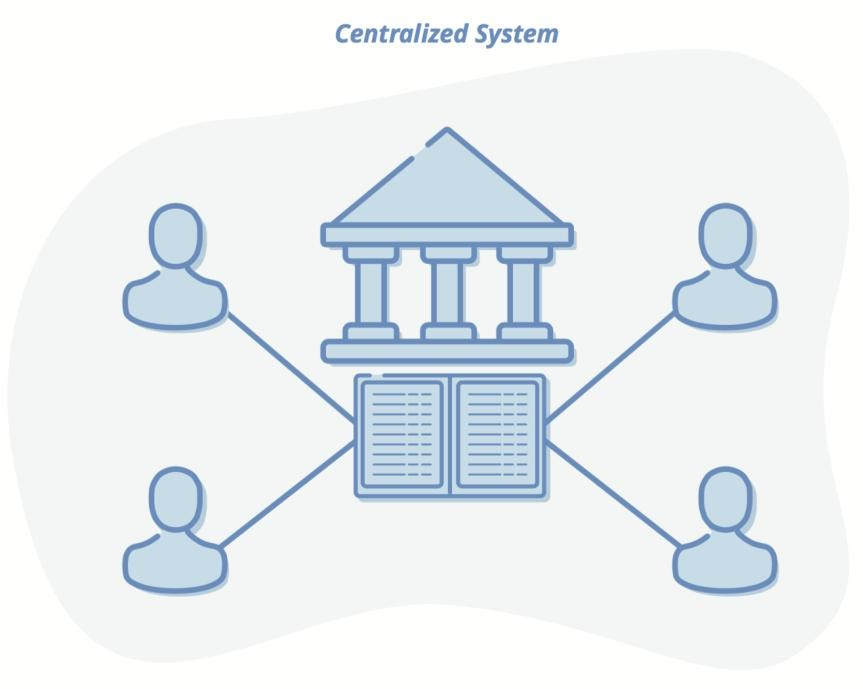
\includegraphics[width=10cm]{imagens/centralizado-capitulo-02.jpg}
  \caption{Sistema centralizado}
\end{figure}


\paragraph{O problema de gasto duplo}
\paragraph{}

O que acontecerá se Ana tentar gastar esses dois dólares novamente? Isso é chamado de problema de gasto duplo. Ela envia a solicitação para o banco, mas o banco diz “Desculpe, vemos que você já gastou R\$2,00 para pagar Bruno, você não tem mais dinheiro para enviar”.

Quando você tem uma autoridade central como um banco, é muito fácil para ele dizer que você está tentando gastar um dinheiro que já gastou. Isso porque eles são os únicos que podem modificar o livro-razão e têm processos internos, incluindo sistemas de backup e auditorias feitas por computadores e seres humanos para se certificar de que está correto e nada foi adulterado.

Chamamos isso de \textit{sistema centralizado} porque possui um único ponto de controle.

\paragraph{Vamos descentralizar o livro razão}
\paragraph{}

O primeiro problema que o Bitcoin visa resolver é a remoção de um intermediário confiável criando um sistema \textit{ponto a ponto}. Vamos imaginar que os bancos desapareceram e precisamos recriar nosso sistema financeiro. Mas desta vez, não vamos ter um ente central. Como podemos manter um livro-razão sem nenhum centralizador?

Se não temos um guardião do livro-razão, precisaremos que o livro-razão pertença ao povo. \textit{Vive la révolution}. É assim que fazemos.

Primeiro, vários nos reunimos e criamos uma \textit{rede}. Isso apenas significa que temos um jeito de conversar uns com os outros. Digamos que trocamos números de telefone ou contas de Snapchat. Quando Ana quiser enviar dinheiro para Bruno, ao invés de ligar para o banco, ela vai no Snapchat de todos os seus amigos e diz a eles: “Estou enviando R\$2,00 para Bruno”. Todos a reconhecem, respondendo "Legal, entendemos!", e escrevem em suas cópias do livro-razão. A imagem agora tem a seguinte aparência:

~

\begin{figure}
  \centering
  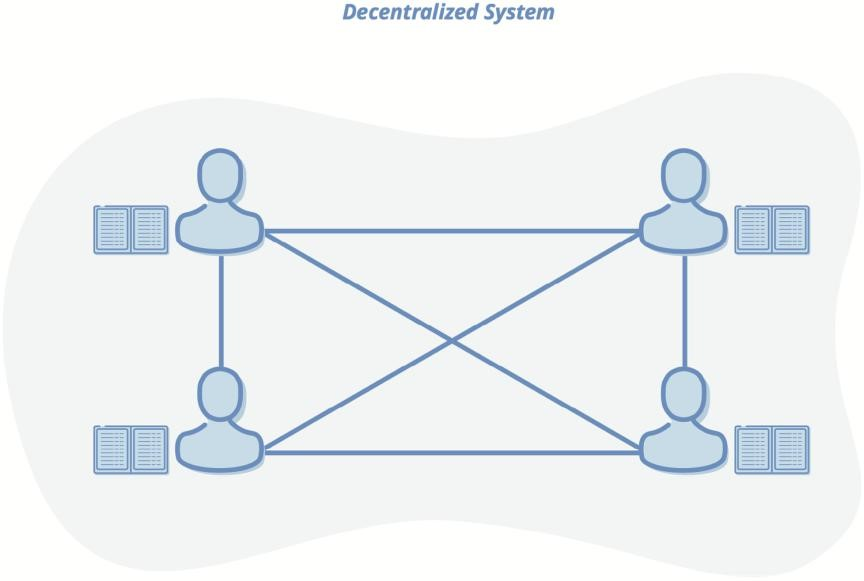
\includegraphics[width=10cm]{imagens/descentralizado-capitulo-02.jpg}
  \caption{Sistema descentralizado}
\end{figure}
\newpage

Portanto, ao invés de um único banco, temos uma cópia do livro-razão nas mãos de todos. Sempre que alguém quer gastar o dinheiro, basta ligar ou fazer um snapchat a todos os seus amigos e informá-los de que isso está acontecendo. Todos registrarão as transações. Como o livro-razão não está mais em apenas um lugar, nós o chamamos de \textit{distribuído} e, como nenhum ente centralizado é responsável, o chamamos de \textit{descentralizado}.

Como isso resolve o problema do gasto duplo? Bem, uma vez que todos possuem uma cópia do livro-razão, se Ana tentar gastar novamente os R\$2,00 que ela já enviou para Bruno, sua transação será rejeitada por todos na rede, já que eles consultariam seus livros-razão e diriam a ela que de acordo com seus registros, ela já gastou o dinheiro.

Agora temos uma rede ponto a ponto para registrar propriedade e transferências de fundos. Este sistema funciona muito bem entre um grupo de amigos que têm motivos sociais para não enganar uns aos outros, mas isso não se aplica quando as redes possuem milhões de pessoas. À medida que mais e mais pessoas começam a usar o sistema, há um incentivo para trapacear para obter dinheiro extra no livro-razão.

Como mantemos todos honestos?
%\part{Sem Confiança e Permissão}
\chapter{Prova de Trabalho}
\label{ch:capitulo3}

%Contanto que nosso livro-razão distribuído exija permissão para participar e possamos confiar que todas as partes sejam honestas, o sistema funcionará. Mas este tipo de design não pode ser escalado para ser usado por milhões de pessoas em todo o mundo.

%Os sistemas distribuídos feitos de participantes arbitrários são inerentemente não confiáveis. Algumas pessoas podem sair ocasionalmente. Isso significa que eles podem não saber das nossas transações quando as transmitimos. Outros podem estar ativamente tentando nos fraudar, dizendo que certas transações aconteceram ou não. Novas pessoas podem ingressar na rede e obter cópias conflitantes do livro-razão. Vamos dar uma olhada em como alguém pode tentar trapacear.%


%\newpage
%no meu livro esse paragrafo separa o inicio do capitulo 3 'prova de trabalho'

%\section**{O sistema de loteria que se auto executa}
%\paragraph{}

Este sistema de loteria, conforme projetado, tem dois problemas principais:

\begin{samepage}
\begin{enumerate}
\item Quem vai vender os bilhetes da loteria e escolher os números vencedores, se já determinamos que não podemos ter nenhum tipo de centralização que possa comprometer sua administração?
\item Como podemos garantir que o vencedor da loteria realmente registre boas transações no livro-razão, ao invés de tentar enganar o resto de nós?
\end{enumerate}
\end{samepage}

Se quisermos um sistema \textit{sem permissão} ao qual qualquer pessoa possa ingressar, temos que remover o requisito de confiança do sistema deixando-o totalmente \textit{sem necessidade de confiança}. Temos que criar um sistema que tenha as seguintes propriedades:


\begin{enumerate}
\item Deve ser possível para todos os integrantes gerar seus próprios bilhetes de loteria, uma vez que não podemos confiar em uma autoridade central;%removido a parte do powerball imagino q pq nao faz sentido em ptbr
\item Precisamos de alguma maneira para que haja custo ao gerar um bilhete, assim evitando que alguém possa monopolizar a loteria gerando um numero alto de bilhetes de graça. Como fazemos que uma possa precise gastar dinheiro para gerar um bilhete quando não há de quem comprar o bilhete? Faremos você comprar o bilhete do universo, queimando energia, um recurso custoso;
%Deve ser fácil para todos os outros participantes verificar se você ganhou na loteria apenas examinando seu bilhete, uma vez que não podemos confiar em ninguém para manter um registro da combinação vencedora;
\item Deve ser fácil para todos os outros participantes verificar se você ganhou na loteria apenas examinando seu bilhete, uma vez que não podemos confiar em ninguém para manter um registro da combinação vencedora, se ao invés disso, combinamos com antecedência uma faixa de valores se seu bilhete estiver dentro dessa faixa você ganha a loteria, usaremos uma ferramenta criptográfica chamada 'função Hash' para fazer isso;

%Precisamos de alguma forma de puni-lo se você ganhar na loteria, mas escrever transações inválidas no livro-razão, substituindo a confiança em pessoas específicas por confiança em incentivos e punições.
\end{enumerate}


%Na minha versao do livro nao tem essa explicação adicional sobre o powerball ela ta incluida na listagem acima.

Vamos falar de todos eles, um de cada vez. A explicação completa de como essa loteria funciona é provavelmente a coisa mais difícil de entender no Bitcoin, então vamos dedicar os próximos três capítulos para cobrir a solução em profundidade.

Sistemas de loteria centralizados padrão como Megasena são executados por alguém gerando um conjunto aleatório de números e um monte de bilhetes com números aleatórios neles. Normalmente, apenas um jogo possui os números que correspondem exatamente ao número aleatório secreto conhecido apenas pela organização que administra a Megasena. Uma vez que não podemos confiar na autoridade central, devemos permitir que qualquer um gere seus próprios números aleatórios.

Como iremos verificar o vencedor? Na Megasena, os proprietários da loteria conhecem a combinação vencedora. Já que não podemos ter isso em um sistema descentralizado, podemos então, criar um sistema onde todos possam concordar em uma faixa de números com antecedência, e se o seu número aleatório cair dentro da faixa, você ganha na loteria. Usaremos um truque criptográfico chamado função hash, para fazer isso. Vamos mergulhar em uma leve introdução a como usar o hash no próximo capítulo.

Finalmente, devemos encontrar uma maneira de puni-lo se você trapacear. Gerar números aleatórios, ou seja, bilhetes de loteria, é basicamente gratuito. Como fazemos para que você realmente tenha que gastar dinheiro para comprar bilhetes quando não há ninguém para vendê-los? Faremos você comprá-los do universo, gastando energia, um recurso escasso que não pode ser criado do nada. Isso será abordado no Capítulo 5.

\section*{Prova de trabalho: um quebra-cabeça assimétrico com uso intensivo de energia}
%\paragraph{}
A solução para esses três problemas é chamada de Prova de Trabalho. Na verdade, foi inventado muito antes do Bitcoin, mais precisamente, em 1993.

Precisamos tornar caro a “compra de bilhetes” para a loteria, caso contrário, as pessoas poderiam gerar um número ilimitado de bilhetes. O que é algo comprovadamente caro, mas isso não precisaria vir de nenhuma autoridade central?

Eu mencionei a física no início do livro, e é aqui que a física joga com o Bitcoin: a primeira lei da termodinâmica diz que a energia não pode ser criada nem destruída. Em outras palavras, não existe almoço grátis quando se trata de energia. A eletricidade é sempre cara porque é um recurso escasso que custa dinheiro real. Você tem que comprá-la dos produtores de energia ou operar sua própria usina. Em qualquer caso, você não pode obter algo do nada.

O conceito por trás da Prova de Trabalho é que você participa de um processo aleatório, semelhante a lançar um dado. Mas, em vez de um dado de seis lados, este tem tantos lados quanto a quantidade de átomos que existem no universo. Para lançar o dado e gerar números de loteria, seu computador deve realizar várias operações, que custam em termos de eletricidade.

Para ganhar na loteria, você deve produzir um número especial que é matematicamente derivado das transações que deseja gravar no livro-razão, mais um número aleatório (explicaremos os detalhes de como isso funciona no próximo capítulo).

Para encontrar esse número vencedor, você pode ter que rolar esse dado bilhões, trilhões ou quatrilhões de vezes, queimando centenas ou milhares de dólares em energia. Como o processo é baseado na aleatoriedade, é possível que todos gerem seus próprios bilhetes de loteria sem uma autoridade central, usando basicamente apenas um número aleatório que pode ser gerado por um software ou hardware e uma lista de transações que desejam gravar no livro-razão.

Agora, embora possa ter levado milhares de dólares para utilizar energia suficiente para encontrar o número aleatório correto, para que todos os outros na rede validem que você é um vencedor, eles precisam realizar algumas verificações básicas:

\begin{samepage}
\begin{enumerate}
\item O número que você forneceu é menor ou maior do que o limite mágico com o qual todos concordaram?
\item O número é de fato derivado matematicamente de um conjunto válido de transações que você deseja gravar no livro-razão?
\item As transações que vocês esta registrando são validas perante as regras do Bitcoin: sem gasto duplo, não gerando novos Bitcoin além do previsto e etc.
\end{enumerate}
\end{samepage}
%adicionado 
Prova de trabalho é um processo aleatório que requer muitas computações para achar o numero vencedor. Entretanto requer apenas uma única operação para verificar esta solução. Pense nele como palavras cruzadas ou sudoku. Pode demorar muito tempo para achar uma solução, mas dado as solução é de rápida verificação.
Isso torna o sistema de Prova de Trabalho \textit{assimétrico}: é muito difícil de gerar, mas muito fácil de ser validado.

Como você consumiu uma quantidade considerável de energia, e por sua vez, dinheiro jogando na loteria, deseja que todos aceitem o seu bilhete de loteria premiado. Portanto, você é incentivado a se comportar bem escrevendo apenas transações válidas no livro-razão.

Se você, por exemplo, tentar gastar um dinheiro que já foi gasto, então seu bilhete de loteria "vencedor" será rejeitado por todos os outros, e você perderá todo o dinheiro que gastou comprando a energia para criar o bilhete. Por outro lado, se você escrever transações válidas no livro-razão, iremos recompensá-lo em bitcoin para que você possa pagar suas contas de energia e ainda ter algum lucro.

O sistema de Prova de Trabalho tem a importante propriedade de ser \textit{caro no mundo real}. Assim, se você quisesse atacar a rede coagindo alguns de seus participantes, não só teria que vir à casa deles e assumir o hardware, mas também pagar suas contas de luz.

%Esse trecho nao vai agora na minha versao do livro.( na minha versao ele começa a falar sobre hashing e bits.)
%Hoje, estima-se que a rede Bitcoin como um todo gasta mais energia nesta loteria do que alguns países de médio porte. Essa é a quantidade de energia que você teria que usar para enganar a rede.

%Como os participantes provam que usaram essa energia? Discutiremos como a Prova de Trabalho é validada do ponto de vista matemático, à seguir.

%%%%%%%%%%%%%%%%%%%%%%%%%%%%%%%%%%%%%%%%%%%%%%%%%%%%%%%%%%%%%%%%%%%%%%%%%%%%%%%%%%%%%%%%%%%%%%%%%%%
Antes de podermos discutir como a Prova de Trabalho é validada, precisaremos de uma introdução rápida em Ciência da Computação sobre dois conceitos: bits e criação de hash.

\section*{Criando um Hash}
%\paragraph{}

O quebra-cabeça de Prova de Trabalho assimétrico do Bitcoin envolve o uso de uma função hash. Da álgebra básica, sabemos que uma função é uma caixa onde você \textit{insere} um valor de entrada \textit{x} e obtém um valor de saída \textit{f(x)}. Por exemplo, a função \textit{f(x)=2x} pega um valor e o multiplica por dois. Portanto, a entrada \textit{x=2} nos dá a \textit{saída f(x)=4}.

Uma função hash é uma função especial, onde você insere qualquer sequência de letras, números ou outros dados, como “Olá, mundo”, e obtém um número gigante que parece algo totalmente aleatório:

\begin{quote}{1111811713258219242661329357757490458455 \newline
4890446643616001126584346633541502095
}\end{quote}

A função hash particular usada acima na string "Hello, World" é chamada de sha256 e, por acaso, é a que o Bitcoin usa.

\begin{figure}
  \centering
  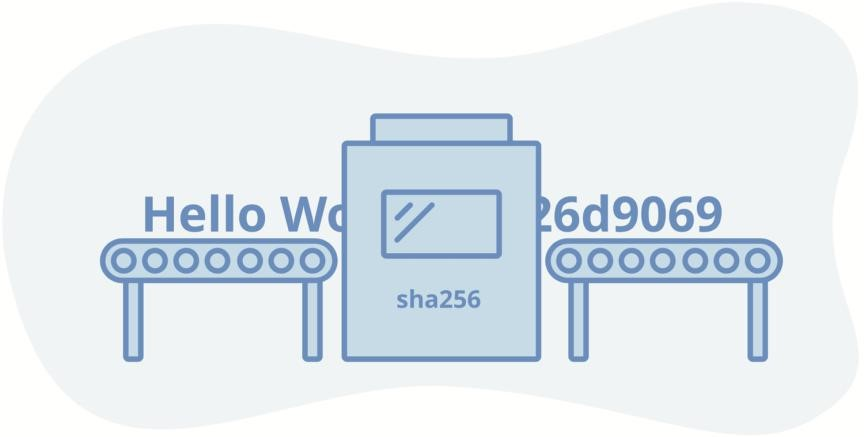
\includegraphics[width=7cm]{imagens/hash-capitulo-04.jpg}
  \caption*{\textit{\small Fazendo o hash de um string}}
\end{figure}

A função hash sha256 tem as seguintes propriedades que são úteis para nós:

\begin{enumerate}
\item A saída é determinística: você sempre obtém a mesma saída para a mesma entrada;
\item A saída é imprevisível: alterar apenas uma letra ou adicionar um espaço à string de entrada mudará drasticamente a saída, tanto que você não pode encontrar nenhuma correlação com os dados de entrada original;
\item É rápido calcular o hash para dados de entrada de qualquer tamanho;
\item É impossível encontrar duas strings que geram hash para a mesma saída;
\item Dado o hash de saída de sha256, é impossível retornar à string de entrada. Chamamos isso de função unilateral;
\item A saída é sempre um tamanho específico (256 bits para sha256).
\end{enumerate}

\section*{Uma introdução rápida sobre bits}
%\paragraph{}

O sistema numérico que você conhece e adora, composto dos números de 0 a 9, é chamado de \textit{decimal} porque possui dez dígitos. Os computadores, por outro lado, preferem um sistema numérico diferente, feito de uns e zeros, indicando a presença ou ausência de um sinal elétrico. Este sistema numérico é chamado de \textit{binário}.

No sistema decimal, você usa apenas os dígitos de 0 a 9. Se você usar apenas um dígito, poderá representar dez números diferentes, de 0 a 9. Se usar dois dígitos, poderá representar 10x10=100 números diferentes: 00, 01,\ldots a 99. Para três dígitos, você pode ter 10x10x10=1000 números: 000, 001,\ldots a 999.

Espero que você esteja começando a ver um padrão. Para descobrir o tamanho de um número que podemos representar com N dígitos, multiplicamos dez por ele mesmo N vezes. Em outras palavras, \(10^N\), ou 10 elevado à potência de N.

O binário funciona da mesma maneira. A única coisa que muda é o número de dígitos que estão disponíveis para nós. Embora estejamos acostumados com decimais com dez dígitos, um \textit{dígito binário} ou \textit{bit} só pode ter dois valores: zero e um.

Se 1 bit pode representar dois valores, então dois bits podem representar 4 valores: 00, 01, 10, 11. Você pode calcular isso multiplicando 2x2, pois cada dígito pode ter dois valores.

Três bits podem representar 2 x 2 x 2 = \(2^3\) = 8 valores, que são 000, 001, 010, 011, 100, 101, 110, 111.

Portanto, um número \textit{binário} de N \textit{bits} pode ser representado como \(2^N\) valores diferentes.

Portanto, o número de valores exclusivos que você pode representar com 256 bits, o tamanho da função de hashing sha256, é \(2^{256}\). Esse é um número gigante, quase inconcebível para a mente humana. Representado em decimal, esse número tem 78 dígitos. Para colocar isso em perspectiva, isso é mais ou menos o número estimado de átomos em todo o universo conhecido.


\begin{multline}
\begin{aligned}
2^{256} = & 115.792.089.237.316.195.423.570.985.008.\\
& 687.907.853.269.984.665.640.564.039.457.\\
& 584.007.913.129.639.936
\end{aligned}
\end{multline}


Este é o número de saídas possíveis quando você faz o hash de qualquer string com a função de hash sha256. Portanto, é efetivamente impossível prever como será o número produzido por essa função. Seria como prever 256 jogadas de moeda em sequência ou adivinhar a localização de um átomo específico que escolhi em algum lugar do universo.

Este número é muito longo para continuar escrevendo, então diremos apenas \(2^{256}\) de agora em diante, mas espero que isso acione uma imagem mental de um universo de possibilidades para você.

\section*{Vamos transformar algumas strings em hash}
%\paragraph{}

Aqui estão algumas strings de exemplo e seus hashes sha256. O resultado está em números decimais, embora dentro de um computador eles apareceriam como uma sequência binária de uns e zeros.

O objetivo aqui é demonstrar como o número muda drasticamente com base em uma pequena mudança na string de entrada. Você não pode prever a saída produzida pela função hash com base no que você colocou nela:


\begin{quote}{"Hello World!"\newline
52740724284578854442640185928423074974\newline
81806529570658746454048816174655413720\newline
}\end{quote}


\begin{samepage}
\begin{quote}{"Hello World!!"\newline
958633198749395357316023441946434972583\newline
74513872780665335270495834770720452323\newline
}\end{quote}
\end{samepage}

Não há como ninguém, nem mesmo um computador, olhar para o número de aparência aleatória resultante e descobrir a string que o criou. Se você quiser brincar com o sha256, há alguns sites online onde você pode experimentar fazer o hash de qualquer informação que desejar. por exemplo \url{https://passwordsgenerator.net/sha256-hash-generator/}

\section*{Criando um hash para ganhar na loteria de prova de trabalho}
%\paragraph{}
 
Tudo bem, agora estamos prontos para falar sobre a parte chave da magia. Dissemos que há \(2^{256}\) valores de saída de sha256 possíveis no total. Para tornar mais fácil de entender, vamos fingir que há apenas um total de 1000 saídas hash possíveis.

O nosso sistema de loteria funciona assim:

\begin{enumerate}
\item Ana anuncia que deseja enviar R\$2,00 para Bruno;
\item Todo mundo que quer tentar a sorte na loteria pega esta transação “Ana envia R\$2,00 para Bruno”, adicionando um número aleatório chamado \textit{nonce} (número usado apenas uma vez) no final. Isso é para ter certeza de que a string que eles estão fazendo o hash é diferente de qualquer outra pessoa, ajudando-os a encontrar um número vencedor na loteria;
\item Se esse número for menor do que o \textit{Número Alvo} (veremos isso em um segundo), eles ganham na loteria;
\item Se o número que eles obtiverem for maior do que o número alvo, eles tentam fazer o hash novamente, adicionando nonces aleatórios: “Ana envia R\$2,00 para Bruno com nonce = 12345”, “Ana envia R\$2,00 para Bruno com nonce = 92435”, “Ana envia R\$2,00 para Bruno nonce = 132849012348092134” e assim por diante, até que o número hash resultante seja menor que o \textit{Número Alvo}.
\end{enumerate}

Pode levar muitas, muitas tentativas para encontrar um hash que seja menor que o número alvo. Portanto, a ideia aqui é esta: se houver 1000 hashes possíveis e definirmos o número alvo como 100, qual porcentagem de hashes está abaixo do alvo?

Esta é a matemática básica: de 1000 números possíveis, de zero a 999, existem 100 números que são menores que 100 e 900 números que são maiores. Portanto, 100/1000 ou 10\% dos hashes são menores que o destino. Então, se você fizer um hash com qualquer string e sua função hash produzir 1000 saídas diferentes, você espera obter um hash abaixo do alvo limitado a 100, cerca de 10\% do tempo.

É assim que a loteria funciona: nós definimos um \textit{alvo} e todos concordamos com ele (falaremos sobre como isso funciona em breve). Então, pegamos as transações sobre as quais as pessoas estão nos contando e fazemos o hash, adicionando um nonce aleatório no final. Assim que alguém encontra um hash que está dentro do limite imposto pelo alvo, nós o anunciamos para todos na rede:

Olá pessoal:
\begin{itemize}
\item Peguei as transações: "Ana envia R\$2,00 para Bruno, Carol envia R\$5,00 para Ana";
\item Adicionei o nonce "32895";
\item O resultado foi um hash com retorno 42, que é menor que o alvo limite de 100;
\item Aqui está minha prova de trabalho: os dados da transação, o nonce que usei e o hash que foi produzido com base nessas entradas.
\end{itemize}

Para isso, talvez seja necessário bilhões de tentativas de hash para conseguir o resultado, gastando milhares de dólares em energia, mas todos podem imediatamente validar que fiz certo porque eles podem fazer o hash em uma única tentativa, já que dei a entrada e o saída esperada. Lembre-se de que os hashes são impossíveis de serem revertidos, mas são fáceis de serem calculados!

Como isso está ligado ao gasto de energia? Bem, já dissemos que o conjunto de todos os hashes possíveis é na verdade um número gigante que é quase tão grande quanto o número de átomos no universo. Agora podemos definir o \textit{alvo} como baixo para que apenas uma pequena fração dos hashes sejam válidos. Isso significa que qualquer pessoa que quiser encontrar um hash válido terá que gastar uma grande quantidade de tempo e processamento o que significa que terá que gastar eletricidade, para encontrar um número de hash menor que nosso alvo.

Quanto menor o alvo, mais tentativas serão necessárias para encontrar um número que funcione. Quanto maior o alvo, mais rápido podemos encontrar um hash vencedor.
% \part{A Matemática do Bitcoin}
% \label{ch:capitulo4}
% \chapter*{A Matemática do Bitcoin}

% Antes de podermos discutir como a Prova de Trabalho é validada, precisaremos de uma introdução rápida em Ciência da Computação sobre dois conceitos: bits e criação de hash.

% \paragraph{Criando um Hash}
% \paragraph{}

% O quebra-cabeça de Prova de Trabalho assimétrico do Bitcoin envolve o uso de uma função hash. Da álgebra básica, sabemos que uma função é uma caixa onde você \textit{insere} um valor de entrada \textit{x} e obtém um valor de saída \textit{f(x)}. Por exemplo, a função \textit{f(x)=2x} pega um valor e o multiplica por dois. Portanto, a entrada \textit{x=2} nos dá a \textit{saída f(x)=4}.

% Uma função hash é uma função especial, onde você insere qualquer sequência de letras, números ou outros dados, como “Olá, mundo”, e obtém um número gigante que parece algo totalmente aleatório:

% \begin{quote}{1111811713258219242661329357757490458455 \newline
% 4890446643616001126584346633541502095
% }\end{quote}

% A função hash particular usada acima na string "Hello, World" é chamada de sha256 e, por acaso, é a que o Bitcoin usa.

% \begin{figure}
%   \centering
%   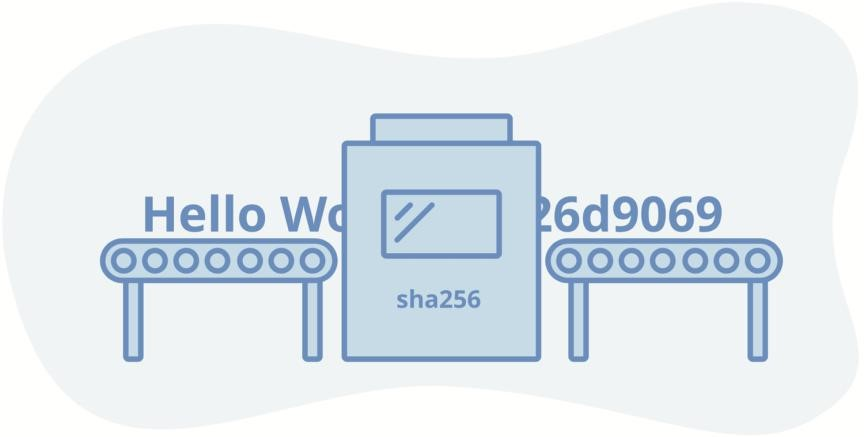
\includegraphics[width=10cm]{imagens/hash-capitulo-04.jpg}
%   \caption{Fazendo o hash de uma string}
% \end{figure}

% A função hash sha256 tem as seguintes propriedades que são úteis para nós:

% \begin{enumerate}
% \item A saída é determinística: você sempre obtém a mesma saída para a mesma entrada;
% \item A saída é imprevisível: alterar apenas uma letra ou adicionar um espaço à string de entrada mudará drasticamente a saída, tanto que você não pode encontrar nenhuma correlação com os dados de entrada original;
% \item É rápido calcular o hash para dados de entrada de qualquer tamanho;
% \item É impossível encontrar duas strings que geram hash para a mesma saída;
% \item Dado o hash de saída de sha256, é impossível retornar à string de entrada. Chamamos isso de função unilateral;
% \item A saída é sempre um tamanho específico (256 bits para sha256).
% \end{enumerate}

% \newpage

% \paragraph{Uma introdução rápida sobre bits}
% \paragraph{}

% O sistema numérico que você conhece e adora, composto dos números de 0 a 9, é chamado de \textit{decimal} porque possui dez dígitos. Os computadores, por outro lado, preferem um sistema numérico diferente, feito de uns e zeros, indicando a presença ou ausência de um sinal elétrico. Este sistema numérico é chamado de \textit{binário}.

% No sistema decimal, você usa apenas os dígitos de 0 a 9. Se você usar apenas um dígito, poderá representar dez números diferentes, de 0 a 9. Se usar dois dígitos, poderá representar 10x10=100 números diferentes: 00, 01,\ldots a 99. Para três dígitos, você pode ter 10x10x10=1000 números: 000, 001,\ldots a 999.

% Espero que você esteja começando a ver um padrão. Para descobrir o tamanho de um número que podemos representar com N dígitos, multiplicamos dez por ele mesmo N vezes. Em outras palavras, \(10^N\), ou 10 elevado à potência de N.

% O binário funciona da mesma maneira. A única coisa que muda é o número de dígitos que estão disponíveis para nós. Embora estejamos acostumados com decimais com dez dígitos, um \textit{dígito binário} ou \textit{bit} só pode ter dois valores: zero e um.

% Se 1 bit pode representar dois valores, então dois bits podem representar 4 valores: 00, 01, 10, 11. Você pode calcular isso multiplicando 2x2, pois cada dígito pode ter dois valores.

% Três bits podem representar 2 x 2 x 2 = \(2^3\) = 8 valores, que são 000, 001, 010, 011, 100, 101, 110, 111.

% Portanto, um número \textit{binário} de N \textit{bits} pode ser representado como \(2^N\) valores diferentes.

% Portanto, o número de valores exclusivos que você pode representar com 256 bits, o tamanho da função de hashing sha256, é \(2^{256}\). Esse é um número gigante, quase inconcebível para a mente humana. Representado em decimal, esse número tem 78 dígitos. Para colocar isso em perspectiva, isso é mais ou menos o número estimado de átomos em todo o universo conhecido.


% \begin{multline}
% \begin{aligned}
% 2^{256} = & 115.792.089.237.316.195.423.570.985.008.\\
% & 687.907.853.269.984.665.640.564.039.457.\\
% & 584.007.913.129.639.936
% \end{aligned}
% \end{multline}


% Este é o número de saídas possíveis quando você faz o hash de qualquer string com a função de hash sha256. Portanto, é efetivamente impossível prever como será o número produzido por essa função. Seria como prever 256 jogadas de moeda em sequência ou adivinhar a localização de um átomo específico que escolhi em algum lugar do universo.

% Este número é muito longo para continuar escrevendo, então diremos apenas \(2^{256}\) de agora em diante, mas espero que isso acione uma imagem mental de um universo de possibilidades para você.

% \paragraph{Vamos transformar algumas strings em hash}
% \paragraph{}

% Aqui estão algumas strings de exemplo e seus hashes sha256. O resultado está em números decimais, embora dentro de um computador eles apareceriam como uma sequência binária de uns e zeros.

% O objetivo aqui é demonstrar como o número muda drasticamente com base em uma pequena mudança na string de entrada. Você não pode prever a saída produzida pela função hash com base no que você colocou nela:

% \begin{samepage}
% \begin{quote}{"Hello World!"\newline
% 52740724284578854442640185928423074974\newline
% 81806529570658746454048816174655413720\newline
% }\end{quote}
% \end{samepage}

% \begin{samepage}
% \begin{quote}{"Hello World!!"\newline
% 958633198749395357316023441946434972583\newline
% 74513872780665335270495834770720452323\newline
% }\end{quote}
% \end{samepage}

% Não há como ninguém, nem mesmo um computador, olhar para o número de aparência aleatória resultante e descobrir a string que o criou. Se você quiser brincar com o sha256, há alguns sites online onde você pode experimentar fazer o hash de qualquer informação que desejar. por exemplo \url{https://passwordsgenerator.net/sha256-hash-generator/}

% \paragraph{Criando um hash para ganhar na loteria de prova de trabalho}
% \paragraph{}
 

% Tudo bem, agora estamos prontos para falar sobre a parte chave da magia. Dissemos que há \(2^{256}\) valores de saída de sha256 possíveis no total. Para tornar mais fácil de entender, vamos fingir que há apenas um total de 1000 saídas hash possíveis.

% O nosso sistema de loteria funciona assim:

% \begin{enumerate}
% \item Ana anuncia que deseja enviar R\$2,00 para Bruno;
% \item Todo mundo que quer tentar a sorte na loteria pega esta transação “Ana envia R\$2,00 para Bruno”, adicionando um número aleatório chamado \textit{nonce} (número usado apenas uma vez) no final. Isso é para ter certeza de que a string que eles estão fazendo o hash é diferente de qualquer outra pessoa, ajudando-os a encontrar um número vencedor na loteria;
% \item Se esse número for menor do que o \textit{Número Alvo} (veremos isso em um segundo), eles ganham na loteria;
% \item Se o número que eles obtiverem for maior do que o número alvo, eles tentam fazer o hash novamente, adicionando nonces aleatórios: “Ana envia R\$2,00 para Bruno com nonce = 12345”, “Ana envia R\$2,00 para Bruno com nonce = 92435”, “Ana envia R\$2,00 para Bruno nonce = 132849012348092134” e assim por diante, até que o número hash resultante seja menor que o \textit{Número Alvo}.
% \end{enumerate}

% Pode levar muitas, muitas tentativas para encontrar um hash que seja menor que o número alvo. Portanto, a ideia aqui é esta: se houver 1000 hashes possíveis e definirmos o número alvo como 100, qual porcentagem de hashes está abaixo do alvo?

% Esta é a matemática básica: de 1000 números possíveis, de zero a 999, existem 100 números que são menores que 100 e 900 números que são maiores. Portanto, 100/1000 ou 10\% dos hashes são menores que o destino. Então, se você fizer um hash com qualquer string e sua função hash produzir 1000 saídas diferentes, você espera obter um hash abaixo do alvo limitado a 100, cerca de 10\% do tempo.

% É assim que a loteria funciona: nós definimos um \textit{alvo} e todos concordamos com ele (falaremos sobre como isso funciona em breve). Então, pegamos as transações sobre as quais as pessoas estão nos contando e fazemos o hash, adicionando um nonce aleatório no final. Assim que alguém encontra um hash que está dentro do limite imposto pelo alvo, nós o anunciamos para todos na rede:

% Olá pessoal:
% \begin{itemize}
% \item Peguei as transações: "Ana envia R\$2,00 para Bruno, Carol envia R\$5,00 para Ana";
% \item Adicionei o nonce "32895";
% \item O resultado foi um hash com retorno 42, que é menor que o alvo limite de 100;
% \item Aqui está minha prova de trabalho: os dados da transação, o nonce que usei e o hash que foi produzido com base nessas entradas.
% \end{itemize}

% Para isso, talvez seja necessário bilhões de tentativas de hash para conseguir o resultado, gastando milhares de dólares em energia, mas todos podem imediatamente validar que fiz certo porque eles podem fazer o hash em uma única tentativa, já que dei a entrada e o saída esperada. Lembre-se de que os hashes são impossíveis de serem revertidos, mas são fáceis de serem calculados!

% Como isso está ligado ao gasto de energia? Bem, já dissemos que o conjunto de todos os hashes possíveis é na verdade um número gigante que é quase tão grande quanto o número de átomos no universo. Agora podemos definir o \textit{alvo} como baixo para que apenas uma pequena fração dos hashes sejam válidos. Isso significa que qualquer pessoa que quiser encontrar um hash válido terá que gastar uma grande quantidade de tempo e processamento o que significa que terá que gastar eletricidade, para encontrar um número de hash menor que nosso alvo.

% Quanto menor o alvo, mais tentativas serão necessárias para encontrar um número que funcione. Quanto maior o alvo, mais rápido podemos encontrar um hash vencedor.


\chapter{Minerando}
\label{ch:capitulo5}
%\setcounter{chapter}{5}

%O processo de jogar na loteria da prova de trabalho para ganhar o direito de escrever na livro de registros do Bitcoin é popularmente conhecido como mineração e é assim que funciona:
O processo de jogar na loteria de Prova de Trabalho para ganhar acesso e escrever o livro-razão do Bitcoin é popularmente conhecido como \textit{mineração}.
Agora estamos prontos para ver como a loteria de prova de trabalho do Bitcoin realmente funciona:

\begin{enumerate}
\item Qualquer pessoa que desejar participar, entra na rede Bitcoin conectando seu computador e ouve as transações;
\item Ana anuncia sua intenção de enviar algumas moedas para Bruno. Os computadores da rede ficam conversando entre si para espalhar essa transação para todos demais usuários;
\item Todos os computadores que desejam participar da loteria começam a fazer o hash das transações que ouviram falar, acrescentando os nonces aleatórios à transação e executando as funções do hash sha256;
\item Aproximadamente a cada dez minutos, algum computador a encontra um número hash menor que o número alvo atual ganha a loteria;
\item Este computador anuncia o número vencedor que eles encontraram e a entrada (transações e nonce) que eles usaram para produzi-lo. Pode ter levado horas para conseguir, ou alguns minutos. Essas informações juntas (transações, nonce e hash da Prova de Trabalho) são chamadas de \textit{bloco};
\item Todos os outros validam o bloco verificando se as transações junto com o nonce do hash de fato geram aquele determinado hash, e se ele é de fato menor que o \textit{Número Alvo} e se o bloco não contém nenhuma transação inválida, e que a história dentro dele não conflita com blocos anteriores;
\item Todos escrevem o bloco em sua cópia do livro-razão, acrescentando-o à cadeia de blocos existente, produzindo uma \textit{blockchain}.
\end{enumerate}

É isso. Produzimos nosso primeiro bloco e nossa primeira entrada em nossos livros-razão.

Talvez você já tenha lido em algum lugar da mídia que minerar Bitcoins envolve solucionar equações complexas. Agora você entende que isso é falso. Invés de solucionar equações, a loteria de mineração de Bitcoin é sobre jogar um dado gigante repetidas vezes para produzir um hash dentro de um dado intervalo. É simplesmente um jogo de azar, que força os participantes a gastarem uma certa quantia de eletricidade. 

\section*{Como são minerados novos bitcoins?}

Até agora, discutimos como Ana pode enviar R\$2,00 para Bruno. Vamos parar de falar em reais, porque o Bitcoin não sabe nada sobre essa moeda. O que temos são os próprios bitcoins - unidades digitais que representam valor na rede Bitcoin.

Para revisitar nosso exemplo, o que realmente está acontecendo é que Ana está enviando 2 bitcoins para Bruno, anunciando que ela está movendo bitcoins que estão registrados na sua “conta” para a conta de Bruno. Alguém então ganha na loteria de Prova de Trabalho e escreve sua transação no livro-razão.

Mas onde Ana conseguiu esses 2 bitcoins para começo de conversa? Como o Bitcoin começou e como alguém adquiriu o Bitcoin antes de haver lugares para comprá-lo com a moeda fiduciária tradicional, como o real brasileiro?

%faltou esse paragrafo
Quando Satoshi criou o Bitcoin, ele podia ter criado um banco de dados no qual ele seria o dono de 21 milhões de moedas e pedido a pessoas comprarem isso dele. Porem, teria-se pouco motivo para pessoas atribuírem valor a um sistema que apenas uma pessoa controla toda a riqueza. Ele poderia criar um registro, onde algumas pessoas poderiam se cadastrar com um e-mail para ter uma chance de ganhar algumas moedas, mas isso seria suscetível a um ataque de Sybil(impersonificação) visto que da para gerar milhões de endereços de e-mails quase que gratuitamente.

Acontece que o processo de mineração de bitcoin, que é o processo de jogar na loteria de Prova de Trabalho e obter direitos de acesso ao livro-razão, é exatamente o que produz mais unidades de bitcoin. Quando você encontra um bloco válido (utilizando uma grande quantidade de energia e encontrando um número que é válido e que te faz vencedor da loteria), você pode escrever todas as transações sobre as quais ouviu falar naquele Bloco e, portanto, no livro-razão.%removido espaço
Mas você também pode gravar uma transação adicional muito especial, chamada de transação \textit{coinbase} (ou transação de cunhagem no português) no livro-razão. Essa transação basicamente diz: "12,5 Bitcoins foram criados e dados a Maria, a mineradora, para compensá-la por gastar toda aquela energia para minerar este bloco".

%faltou esse paragrafo
É assim que novos bitcoins são minerados a existência. esse processo permite absolutamente qualquer pessoa no mundo de minerar seus próprios bitcoins sem a existência de uma autoridade central, e sem identificar a eles mesmos, contanto que estejam dispostos a pagar pelo custo da eletricidade necessário para participar da loteria. Isso torna Bitcoin resistente a ataque de Sybil. Se você quiser moedas terás que gastar energia e pagar um dinheiro para minerar elas.

\section*{A recompensa do bloco}

Assim, a pessoa que ganha na loteria pode dar a si mesma alguns bitcoins recém criados. Mas por que 12,5 bitcoin e não 1000? Por que ela não pode enganar o sistema e dar a si mesma qualquer quantia? 

Aqui está a parte principal: O Bitcoin é um sistema de consenso distribuído. Isso significa que todos devem concordar sobre o que é válido. A maneira que se faz isso é através de rodar um software no computador que aplica um grupo de regras bem definidas, conhecidas como as regras de consenso do Bitcoin. Qualquer bloco produzido por mineradores é validado por essas regras. Se ele passar, todos irão escrever em seus livros razão e aceitar como a verdade. Se não o bloco é rejeitado.

embora a lista completa de regras de consentimento seja um tanto complexa, aqui estão alguns exemplos.
%adicionado
\begin{itemize}
    \item  Um bloco valido pode criar uma quantia especifica de Bitcoins, determinada pelo cronograma de emissão que esta escrito no código
    \item  Transações precisam ter assinaturas corretas, indicando que as pessoas que estão gastando aquelas moedas tem a autorização devida.
    \item Não é permitido ter transações que gastam moedas que haviam sido gastas anteriormente nesse bloco ou qualquer outro bloco anterior.
    \item A informação contida em um bloco não pode ser maior que um determinado tamanho.
    \item O hash de prova de trabalho precisa ser inferior ao atual tamanho alvo, provando a improbabilidade estatística desse bloco ter sido minerado utilizando qualquer outro método que não o gasto de uma certa quantidade de energia.
\end{itemize}
%

Se Maria criar um bloco e decidir dar a si mesma algo além desta quantidade, o computador de todos os outros \textit{rejeitará} o bloco como sendo inválido, porque dentro do software do Bitcoin Client que todos estão executando, há um trecho de código que diz "a recompensa do bloco atual é exatamente 12,5 bitcoin. Se você receber um bloco que concede a alguém mais do que isso, não aceite”.

Se Maria tentar trapacear e produzir um bloco \textit{inválido}, o bloco não será gravado no livro-razão de ninguém e ela terá desperdiçado milhares de dólares em eletricidade produzindo algo que ninguém aceitará, ou seja, uma falsificação.
%adicionado
Isso concede ao Bitcoin uma custo infalsificável(\textit{unforgeable costliness}), um termo usado primeira vez pelo pioneiro em moedas digitais, Nick Szabo, no seu artigo \textit{Shelling Out}. Intuitivamente sabemos que se dinheiro fosse fácil de falsificar, não seria muito útil como dinheiro. Bitcoin é tão impossível de se falsificar, quanto é fácil de testar, através de um simples verificação matemática.
  
%modificado
O primeiro bloco minerado foi criado por Satoshi. O código é de código aberto - isso significa que qualquer pessoa pode dar uma olhada em como ele funciona e validar que nada de suspeito está acontecendo por detrás dos panos. Até o Satoshi teve que fazer cálculos e jogar na loteria de Prova de Trabalho para extrair o primeiro bloco.
Ele mesmo não poderia produzir uma falsificação, fraudando o custo de energia, embora ele seja o criador do sistema.

%adicionado
Qualquer pessoa que se juntou a rede depois dele pode verificar o hash que ele gerou com alvo inicial e os dados da transição para notar que ele havia atingindo o alvo estatisticamente raro através do gasto de energia. Imagine ser capaz de auditar a criação de dinheiro do tradicional sistema bancário fiat nesse nível de precisão e em tempo real.

\section*{O Halving}
%adicionado
O processo de mineração produz novos Bitcoins. Mas Satoshi queria um sistema que não era possível de ser depreciar. Ele não queria que a oferta monetária pudesse ser perpetuamente expandida. Invés, ele projetou um cronograma de emissão de novas moedas que começava muitas e tendia a zero novas moedas por ano.

No início, a recompensa do bloco era de 50 bitcoin, então foi isso que Satoshi ganhou por minerar o primeiro bloco, assim como as outras pessoas que se juntaram à rede nos primeiros dias depois dos primeiros blocos serem criados.

O código Bitcoin impõe que cada recompensa do bloco seja reduzida pela metade a cada quatro anos aproximadamente. Isso se baseia na quantidade de blocos minerados, e não na passagem do tempo, mas eles são quase os mesmos devido aos blocos sendo produzidos aproximadamente a cada dez minutos.

A Recompensa por Bloco em 2009 foi de 50, em 2012 foi de 25, em 2016 foi de 12,5. A partir de hoje, 15 de janeiro de 2019 - foram minerados 558.688 blocos, desde o início da história do Bitcoin, e a recompensa é de 12,5 bitcoin por bloco.

71.312 blocos a partir deste momento, ou aproximadamente no final de maio de 2020, a recompensa será reduzida para 6,25 bitcoins por bloco, levando a uma inflação do fornecimento anual de moedas para aproximadamente 1,8\%. Uma década depois, após dois halvings, mais de 99\% de todo o Bitcoin terá sido minerado e menos de 1 bitcoin será produzido por bloco. Você pode monitorar o processo de halving em \url{https://www.bitcoinblockhalf.com/}

\begin{figure}[htb]
  \centering
  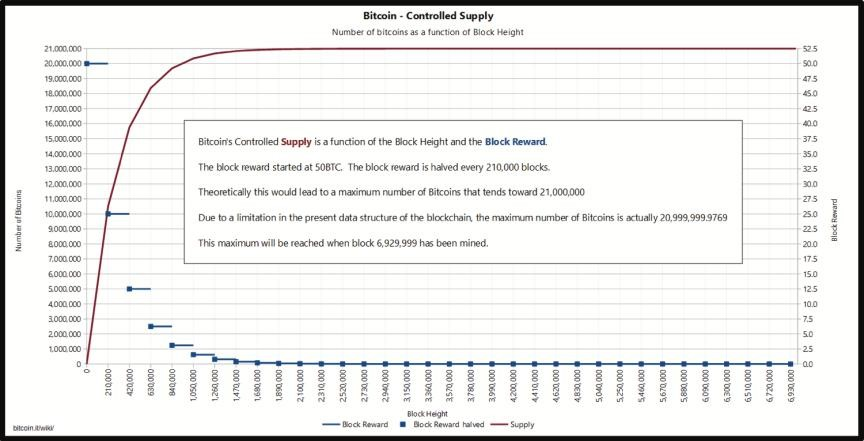
\includegraphics[width=10cm]{imagens/grafico-capitulo-05.jpg}
  \caption*{\textit{\small \url{https://en.bitcoin.it/w/images/en/4/42/Controlled_supply-supply_over_block_height.png}}}
\end{figure}

Eventualmente, por volta do ano 2140, a Recompensa por Bloco desaparecerá totalmente, e os mineradores serão incentivados apenas pelas taxas pagas por aqueles que realizam as transações.

Esses números de emissão e de recompensa de bloco são aplicados no código Bitcoin - que, para reiterar, é totalmente de código aberto e pode ser validado por qualquer pessoa - dependendo de quão longe estamos na história do Bitcoin, produzindo um bloco que não siga essas regras fará com que você seja rejeitado por todos os outros que estão verificando as mesmas que estão escritas em seus códigos.

\section*{Controlando a Emissão e Intervalo de Mineração}


A mineração requer hardware e eletricidade, portanto, quanto mais hardware e eletricidade você controlar, maior será a probabilidade de encontrar o resultado mais rápido, em comparação às demais pessoas. Por exemplo, se houver 100 computadores com velocidade e custo energético igual na rede e você controlar 10 deles, encontrará o bloco vencedor em \textit{aproximadamente} 10\% das vezes. No entanto, a mineração é um processo baseado no acaso e na aleatoriedade, então é possível que horas ou mesmo dias possam se passar sem que você encontre um bloco.

Como foi falado na seção anterior, os mineradores não podem simplesmente conceder a si mesmos recompensas de blocos arbitrárias, ou seriam rejeitados pelos demais nodes. Mas e se eles gastarem muita energia para adiantar os blocos de mineração e colocarem as mãos em um monte de bitcoins, violando a restrição do projeto de que o cronograma de emissão deve ser conhecido com antecedência?

Vamos novamente ao exemplo de que há apenas 1000 hashes possíveis e nosso número de alvo sendo 100. Isso significa que 10\% das vezes vamos lançar um número menor que 100 e encontrar um bloco.

Digamos que leve 1 segundo para calcular cada hash. Se a cada segundo "lançarmos nosso dado" \  misturando as transações atuais e nosso nonce aleatório, e 10\% das vezes atingirmos um número menor que o alvo, então esperamos que leve cerca de 10 segundos, em média, para encontrar um hash válido.

O que acontece se dois computadores estiverem apostando nessa loteria? Eles têm duas vezes mais hashes sendo tentados, então esperamos que um hash válido seja encontrado em 5 segundos. E se 10 computadores estiverem jogando? Um deles encontrará um hash válido aproximadamente a cada segundo.

Isso cria um problema: se mais pessoas estão minerando, os blocos serão produzidos muito rapidamente. Isso gera dois resultados que não queremos:

\begin{enumerate}
\item Isso atrapalha a ideia de ter um cronograma de emissão pré-determinado. Queremos que seja emitido um número relativamente consistente de bitcoins por hora para ter certeza de que emitiremos todos eles até o ano 2140, e não antes disso;
\item Isso cria problemas de rede: se os blocos são extraídos tão rapidamente que não têm tempo de alcançar toda a rede antes que o próximo seja extraído, então não podemos chegar a um consenso sobre uma história linear de transações, uma vez que vários mineradores podem incluir a mesma transação em seus blocos, fazendo com que os blocos sejam inválidos por conterem transações que já foram gastas em outros blocos.
\end{enumerate}

E se menos pessoas estão minerando, criamos o problema oposto:

\begin{enumerate}
\item Os bitcoins estão sendo emitidos muito lentamente, novamente interferindo na emissão pré-determinada;
\item A blockchain pode se tornar inutilizável conforme as pessoas esperam horas, dias ou até mesmo semanas, para obter uma transação gravada no livro-razão.
\end{enumerate}


O número total de hashes por segundo executado por todos os mineradores da rede Bitcoin é conhecido como \textit{hash rate}.

\begin{figure}[htb]
  \centering
  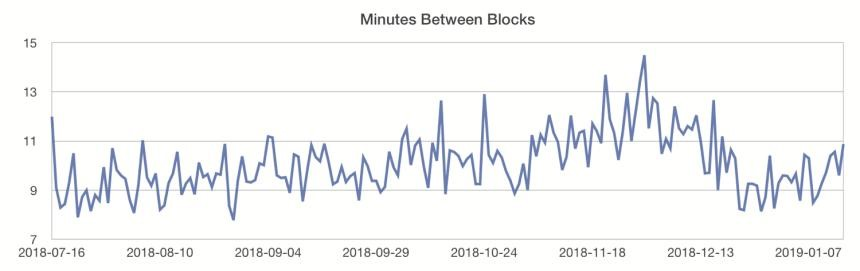
\includegraphics[width=10cm]{imagens/grafico2-capitulo-05.jpg}
  \caption*{\textit{\small Minutos entre blocos minerados}}
\end{figure}




\section*{Ajustes de dificuldade: concordando com o alvo}

%adicionado
Como Bitcoin é um sistema voluntario e sem permissão que pessoas podem participar quando desejarem, sem ninguém comandando, o numero de mineradores ativos em um dado momento pode variar drasticamente. Precisamos de uma maneira de manter a produção de blocos estável impedindo aumentos ou reduções no cronograma toda vez que um minerador novo entra na rede ou um minerador existente saia.

%da uma olhada na ultima frase do paragrafo a seguir Korea!!
%...if players leave the lottery, in order to keep the issuance and block times steady?

Como podemos tornar mais difícil encontrar hashes válidos se mais jogadores entrarem na loteria e mais fácil se os jogadores saírem dela, a fim de manter os tempos de emissão e de blocos estáveis?

%adicionado
Lembre que mineração de Bitcoin é uma loteria para tentar produzir um numero aleatório menor que um alvo.

\begin{figure}
  \centering
  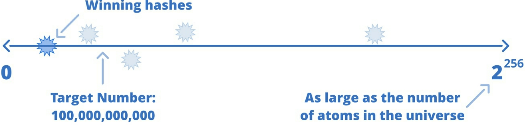
\includegraphics[width=10cm]{imagens/capitulo5/difficulty1.png}
  \caption*{\textit{\small Estamos tentando acertar esse pequeno espaço, o numero de possíveis resultados é grande, que irá demorar uma quantidade grande quantia de tempo para acerta la aleatoriamente.}}
\end{figure}

O Bitcoin resolve esse problema com um \textit{ajuste de dificuldade de mineração}. Como todos estão executando o mesmo código, que impõe as mesmas regras, e todos têm uma cópia de todo o histórico de blocos até este ponto, todos podem calcular de forma independente a rapidez com que os blocos estão sendo produzidos.

A cada 2016 blocos, o que leva aproximadamente o equivalente a duas semanas, olhamos para trás e descobrimos quanto tempo levou para produzir esses blocos e, em seguida, ajustamos nosso \textit{Número Alvo} para acelerar ou desacelerar a produção de blocos.

Todos os usuários pegam os últimos 2016 blocos e os dividem pelo tempo que levaram para produzir, criando assim uma média. Demorou mais de dez minutos? Estamos indo muito devagar. Demorou menos de dez minutos? Estamos indo rápido demais.

Agora podemos fazer um ajuste no \textit{Número Alvo} para que seja aumentado ou diminuído proporcionalmente a quanto mais rápido ou mais devagar queremos ir com base no intervalo de 10 minutos que está escrito no código fonte.

Podemos aumentar o \textit{Número Alvo} para um número mais alto, criando um espaço maior de hashes válidos, dando aos mineradores uma chance maior de encontrar um hash vencedor, gastando menos energia. Isso é chamado de \textit{redução da dificuldade}.
%faltou figura?

\begin{figure}
  \centering
  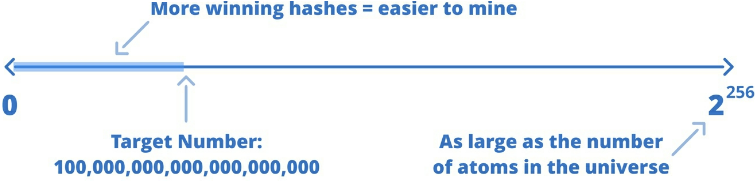
\includegraphics[width=10cm]{imagens/capitulo5/difficulty2.png}
  \caption*{\textit{\small Estamos tentando acertar esse pequeno espaço, o numero de possíveis resultados é grande, que irá demorar uma quantidade grande quantia de tempo para acerta la aleatoriamente.}}
\end{figure}

 De maneira contrária, podemos diminuir o \textit{Número Alvo} para que menos hashes sejam válidas e os mineradores tenham que gastar mais energia para encontrar um hash válido. Isso é chamado de \textit{aumento de dificuldade}.

Isso também significa que, para qualquer bloco, com base em quantos blocos vieram antes dele (a \textit{altura do bloco}), sabemos exatamente qual é o número alvo. Isso nos permite saber o limite mágico sob o qual o número do hash da Prova de Trabalho deve cair para um bilhete de loteria vencedor naquele bloco específico ser dado como válido.

O ajuste de dificuldade e numero alvo é possivelmente a inovação central do Bitcoin, permitindo a qualquer, independentemente, verificar o números da loteria baseados no alvo que eles podem independentemente calcular da mesma maneira que qualquer outra pessoa. É isso que permite a gente rodar uma loteria sem que ninguém nos diga a combinação vencedora.

%Esse paragrafo ta muito diferente do meu para ser o mesmo paragrafo logo defini ele como correto. 


%Isso é brilhante - não precisamos mais de um ente central para nos dizer nada. Tudo o que precisamos fazer é verificar por nós mesmos qual deve ser o Alvo e se a Prova de Trabalho reivindicada por um bilhete de loteria é um número vencedor que está abaixo dele.

O gráfico abaixo mostra a \textit{hash rate} como uma linha e a dificuldade como barras ao longo do tempo. A dificuldade parece uma escada porque é ajustada a cada 2016 blocos. Você pode ver que toda vez que a \textit{hash rate} sobe acima da dificuldade, a dificuldade aumenta para alcançar a \textit{hash rate}. Quando a \textit{hash rate} cai, como aconteceu entre outubro e dezembro de 2018, a dificuldade diminui. O ajuste de dificuldade sempre fica atrás do que quer que a \textit{hash rate} faça.

\begin{figure}
  \centering
  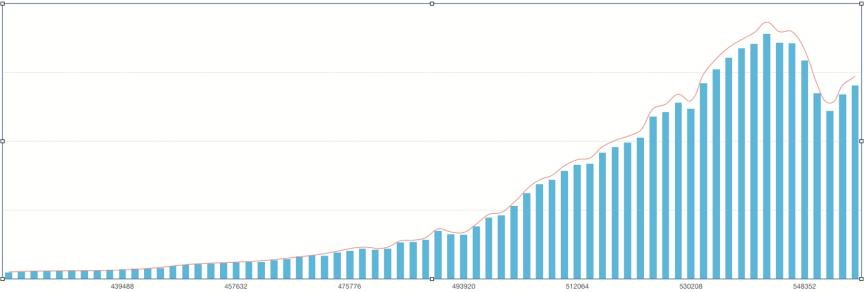
\includegraphics[width=10cm]{imagens/grafico3-capitulo-05.jpg}
  \caption*{\textit{\small Hash Rate em relação a dificuldade}}
\end{figure}

Como há uma defasagem de 2016 blocos entre os ajustes de dificuldade, é possível que haja picos massivos de aumento ou diminuição na \textit{hash rate} para mais ou menos produção de Bitcoin durante o período e isso pode violar levemente o cronograma da emissão.

%nao tem na minha versao

%Na verdade, estamos um pouco mais rápidos agora em comparação com a meta original de finalizar a emissão em 2140. 

Como adicionar \textit{hash rate} normalmente significa produzir uma grande quantidade de novo hardware, isso é relativamente incomum e não afeta muito as coisas, e esperamos que isso se mantenha assim no futuro.
%adicionado
As consequências de qualquer pico são limitadas a uma janela de 2016 blocos, no qual esses picos ocorreram, pois com o próximo ajuste de dificuldade voltaremos a media de 10 blocos por minuto.



\section*{Segurança e o valor em moeda fiduciária do Bitcoin}

Determinamos que o Bitcoin recalcula automaticamente a dificuldade com base no número de jogadores da loteria, ou seja, os mineradores consomem energia quando fazem o hash. É aqui que o mundo real começa a tocar nosso mundo digital. O preço do Bitcoin, o preço do hardware e da energia e o valor de dificuldade criam ciclos de feedback complexos:

\begin{enumerate}
%\item Os mineradores produzem bitcoin consumindo dinheiro para pagar a energia porque acham que as moedas terão algum valor;
\item Os especuladores compram bitcoin porque acham que ele está subindo, elevando o preço para R\$X;
\item Os mineiros gastam até R\$X de energia e hardware para tentar extrair um bitcoin;
\item Uma alta demanda dos compradores e um aumento no preço levam mais mineradores a minerar o bitcoin;
\item Mais mineradores significa mais energia consumida em bitcoin e a rede fica ainda mais segura, tranquilizando os compradores sobre a segurança do Bitcoin, às vezes levando a um ciclo de feedback que aumenta ainda mais o preço;
\item Após a passagem de 2016 blocos, a presença de mais mineradores e, portanto, maior quantidade de hash, causa um ajuste de dificuldade para cima;
\item Uma dificuldade maior significa um Número Alvo menor - os mineradores estão encontrando blocos com menos frequência - fazendo com que pelo menos alguns deles gastem mais R\$X em custos operacionais para extrair uma moeda;
\item Alguns mineradores se tornam não lucrativos, consumindo mais energia na mineração do que podem encontrar de bitcoin, fazendo com que rejeitem ser mineradores;
\item Outros 2016 blocos se passam. A dificuldade é recalculada para ficar mais fácil, já que alguns mineradores saíram do jogo;
\item Uma dificuldade menor significa que os mineiros que antes não eram lucrativos podem voltar a ficar online e fazer a mineração, ou novos mineiros podem entrar no jogo;
\item Vá para o item 1.
\end{enumerate}

Em um mercado em queda, o ciclo pode ir na outra direção, com os usuários vendendo as moedas, fazendo com que o preço caia e os mineiros se tornem não lucrativos.

%nao tem essa primeira frase na minha versao
%No entanto, ao contrário do que se pode ler na mídia sobre uma “espiral da morte”, 
O algoritmo de ajuste de dificuldade garante que sempre haverá algum tipo de equilíbrio entre o preço e o número de mineradores na rede. 
Mesmo que preços despenquem e acabem por remover metade do taxa de hash da rede, na próximo ajuste de dificuldade tornaria mineração lucrativo novamente em torno do novo equilíbrio de preços.

A natureza do ajuste de dificuldade é retirar os mineradores ineficientes em favor dos que operam com a energia mais barata possível. 
Ao longo do tempo, isso força mineradores de bitcoin a partes mais remotas do mundo onde recursos energéticos são abundantes. 
Uma reportagem da \textit{Coinshares} de 2019 estima que 75\% é feito com energias renováveis.

Na prática, nos últimos anos, o preço subiu rapidamente, assim como a taxa total de hash. Quanto mais alta a taxa de hash, mais difícil é atacar a rede porque, para controlar o que é gravado apenas no próximo bloco, é necessário ter muita energia e hardware sob seu controle, pois precisa ter mais da metade de toda a rede. Hoje, a energia utilizada pela rede de mineradores do Bitcoin é estimada como sendo maior do que um país de médio porte.


\section*{Taxas e o fim da recompensa de mineração} 

Se a recompensa de bloco vai eventualmente acabar, como vamos continuar incentivando mineradores a continuamente gastar energia para manter o livro-razão seguro?
A resposta do Bitcoin é taxas de transação financeira.
Não só eles substituem a recompensa de bloco mas incentivam o minerador a incluir transações nos blocos ao invés de minerar blocos vazios.

As taxas são determinadas por um sistema de livre mercado, no qual os usuários pagam por espaço escasso em um bloco. Os usuários que enviam transações indicam quanta taxa estão dispostos a pagar aos mineradores, e eles podem ou não incluir as transações que são informadas, dependendo do quanto irão ganhar. Quando há poucas transações esperando para entrar no próximo bloco, as taxas tendem a ser muito baixas, pois não há competição. À medida que o espaço do bloco é preenchido, os usuários estão dispostos a pagar taxas mais altas para que suas transações sejam confirmadas rapidamente (no próximo bloco). Aqueles que não querem pagar, podem sempre definir taxas baixas e esperar mais para serem minerados em um momento com baixa demanda, quando o espaço do bloco estiver mais disponível.

Ao contrário dos sistemas financeiros tradicionais, onde as taxas tendem a se basear em uma porcentagem do valor que está sendo transferido, no Bitcoin o valor transferido não tem relação com as taxas. Tornamos as taxas proporcionais ao recurso escasso que consomem: espaço em bloco. Portanto, as taxas são medidas em satoshis por byte (bytes são 8 bits, basicamente apenas uma medida de quantos dados há em sua transação). Assim, uma transação que envia um milhão de bitcoins de um endereço para outro pode ser mais barata do que uma que consolida 1 bitcoin espalhado por 10 contas, porque o último requer mais espaço de bloco.

No passado, houve períodos em que o Bitcoin tinha uma demanda muito alta, como o que aconteceu no final de 2017, onde as taxas se tornaram extremamente altas. Desde então, alguns novos recursos foram implementados para reduzir a pressão sobre as taxas na rede.

Uma dessas implementações se chama \textit{Segregated Witness}(ou Testemunha Segregada), que reorganiza como dados no bloco são representados separando as assinaturas digitais dos dados da transação, criando mais espaço para esses dados. Transações que utilizam esse upgrade podem usar mais que 1MB de espaço através de uns truques que estão além do escopo desse livro.

O outro alívio para as taxas veio através do \textit{batching}: As exchanges e outros participantes de alto volume no ecossistema começaram a combinar transações de bitcoin para vários usuários em uma transação. Ao contrário de um pagamento tradicional em seu banco ou PayPal que é feito de uma pessoa para outra, uma transação de Bitcoin pode combinar um grande número de entradas e produzir um grande número de saídas. Assim, uma exchange que precisa enviar bitcoin para saque para 100 pessoas pode fazê-lo em uma única transação. Este é um uso muito mais eficiente do espaço do bloco, transformando o que é ostensivamente apenas um punhado de transações de bitcoin por segundo em milhares de pagamentos por segundo.

\textit{Segragated Witness} e \textit{Batching} já fizeram um bom trabalho em reduzir a demanda por espaço de bloco. Ainda haverá outras melhorias que estão na etapa de desenvolvimento para tornar o espaço no bloco mais eficiente. Mas de qualquer maneira, haverá outros momentos onde as taxas de transações de Bitcoin serão altas novamente devido a alta demanda por espaço de bloco.


Quase concluímos a invenção de todo o Bitcoin:

\begin{enumerate}
\item Substituiu um banco central por um livro-razão distribuído;
\item Instituiu um sistema de loteria para selecionar quem escreve no livro-razão;
\item Os participantes da loteria são forçados a consumir energia para comprar bilhetes por hash e torna mais fácil para todos poderem verificar os bilhetes vencedores, verificando os números hash produzidos pelos jogadores;
\item Diz aos jogadores da loteria que se eles não jogarem de acordo com as regras, rejeitamos os blocos, incluindo as \textit{transações de criação de moedas}, chamadas de \textit{coinbase}, para que eles não fossem pagos quando ganhassem, criando assim um desincentivo econômico para trapacear e um incentivo econômico para jogarem de acordo com as regras;
\item Controlou o tempo e a seleção do \textit{Alvo} para a loteria, permitindo que todos calculassem por si mesmos qual o \textit{Alvo} deveria ser, baseado nas regras codificadas e no histórico dos últimos 2016 blocos;
\item Aplicou o cronograma de emissão usando ajustes de dificuldade que são alterados de acordo com o aumento ou diminuição da \textit{hash rate};
\item Usou o código-fonte aberto para garantir que todos pudessem verificar por si mesmos se estavam aplicando as mesmas regras em relação à validade da transação, recompensa do bloco e cálculo de dificuldade.
\end{enumerate}

%isso esse paragrafo nao tem na minha versao(tirando a primeira e segunda frase(no qual mudei de posição)
% Qualquer um pode participar. Qualquer um pode jogar na loteria e criar bitcoins para si mesmo. Qualquer pessoa pode usar. A produção honesta de blocos é validada por toda a rede e recompensada com uma transação de \textit{coinbase} que paga ao minerador, ou punida por falta de recompensa e o minerador precisa consumir energia na mineração.
 
Não há mais entidade centralizada. Temos um sistema totalmente distribuído e descentralizado.
Quase temos a imagem completa do funcionamento da rede. Resta apenas um problema. Quando alguém se junta à rede e pede cópias do livro-razão, eles podem obter diferentes históricos de nodes diferentes. Como podemos impor uma história única e linear e como podemos evitar que os mineradores reescrevam o passado?




% %\part{Minerando}
% \chapter*{Minerando}
% \label{ch:capitulo5}

\chapter*{Minerando}
\label{ch:capitulo5}
\setcounter{chapter}{5}

%O processo de jogar na loteria da prova de trabalho para ganhar o direito de escrever na livro de registros do Bitcoin é popularmente conhecido como mineração e é assim que funciona:
O processo de jogar na loteria de Prova de Trabalho para ganhar acesso e escrever o livro-razão do Bitcoin é popularmente conhecido como \textit{mineração}.
Agora estamos prontos para ver como a loteria de prova de trabalho do Bitcoin realmente funciona:

\begin{enumerate}
\item Qualquer pessoa que desejar participar, entra na rede Bitcoin conectando seu computador e ouve as transações;
\item Ana anuncia sua intenção de enviar algumas moedas para Bruno. Os computadores da rede ficam conversando entre si para espalhar essa transação para todos demais usuários;
\item Todos os computadores que desejam participar da loteria começam a fazer o hash das transações que ouviram falar, acrescentando os nonces aleatórios à transação e executando as funções do hash sha256;
\item Aproximadamente a cada dez minutos, algum computador a encontra um número hash menor que o número alvo atual ganha a loteria;
\item Este computador anuncia o número vencedor que eles encontraram e a entrada (transações e nonce) que eles usaram para produzi-lo. Pode ter levado horas para conseguir, ou alguns minutos. Essas informações juntas (transações, nonce e hash da Prova de Trabalho) são chamadas de \textit{bloco};
\item Todos os outros validam o bloco verificando se as transações junto com o nonce do hash de fato geram aquele determinado hash, e se ele é de fato menor que o \textit{Número Alvo} e se o bloco não contém nenhuma transação inválida, e que a história dentro dele não conflita com blocos anteriores;
\item Todos escrevem o bloco em sua cópia do livro-razão, acrescentando-o à cadeia de blocos existente, produzindo uma \textit{blockchain}.
\end{enumerate}

É isso. Produzimos nosso primeiro bloco e nossa primeira entrada em nossos livros-razão.

Talvez você já tenha lido em algum lugar da mídia que minerar Bitcoins envolve solucionar equações complexas. Agora você entende que isso é falso. Invés de solucionar equações, a loteria de mineração de Bitcoin é sobre jogar um dado gigante repetidas vezes para produzir um hash dentro de um dado intervalo. É simplesmente um jogo de azar, que força os participantes a gastarem uma certa quantia de eletricidade. 

\section*{Como são minerados novos bitcoins?}

Até agora, discutimos como Ana pode enviar R\$2,00 para Bruno. Vamos parar de falar em reais, porque o Bitcoin não sabe nada sobre essa moeda. O que temos são os próprios bitcoins - unidades digitais que representam valor na rede Bitcoin.

Para revisitar nosso exemplo, o que realmente está acontecendo é que Ana está enviando 2 bitcoins para Bruno, anunciando que ela está movendo bitcoins que estão registrados na sua “conta” para a conta de Bruno. Alguém então ganha na loteria de Prova de Trabalho e escreve sua transação no livro-razão.

Mas onde Ana conseguiu esses 2 bitcoins para começo de conversa? Como o Bitcoin começou e como alguém adquiriu o Bitcoin antes de haver lugares para comprá-lo com a moeda fiduciária tradicional, como o real brasileiro?

%faltou esse paragrafo
Quando Satoshi criou o Bitcoin, ele podia ter criado um banco de dados no qual ele seria o dono de 21 milhões de moedas e pedido a pessoas comprarem isso dele. Porem, teria-se pouco motivo para pessoas atribuírem valor a um sistema que apenas uma pessoa controla toda a riqueza. Ele poderia criar um registro, onde algumas pessoas poderiam se cadastrar com um e-mail para ter uma chance de ganhar algumas moedas, mas isso seria suscetível a um ataque de Sybil(impersonificação) visto que da para gerar milhões de endereços de e-mails quase que gratuitamente.

Acontece que o processo de mineração de bitcoin, que é o processo de jogar na loteria de Prova de Trabalho e obter direitos de acesso ao livro-razão, é exatamente o que produz mais unidades de bitcoin. Quando você encontra um bloco válido (utilizando uma grande quantidade de energia e encontrando um número que é válido e que te faz vencedor da loteria), você pode escrever todas as transações sobre as quais ouviu falar naquele Bloco e, portanto, no livro-razão.%removido espaço
Mas você também pode gravar uma transação adicional muito especial, chamada de transação \textit{coinbase} (ou transação de cunhagem no português) no livro-razão. Essa transação basicamente diz: "12,5 Bitcoins foram criados e dados a Maria, a mineradora, para compensá-la por gastar toda aquela energia para minerar este bloco".

%faltou esse paragrafo
É assim que novos bitcoins são minerados a existência. esse processo permite absolutamente qualquer pessoa no mundo de minerar seus próprios bitcoins sem a existência de uma autoridade central, e sem identificar a eles mesmos, contanto que estejam dispostos a pagar pelo custo da eletricidade necessário para participar da loteria. Isso torna Bitcoin resistente a ataque de Sybil. Se você quiser moedas terás que gastar energia e pagar um dinheiro para minerar elas.

\section*{A recompensa do bloco}

Assim, a pessoa que ganha na loteria pode dar a si mesma alguns bitcoins recém criados. Mas por que 12,5 bitcoin e não 1000? Por que ela não pode enganar o sistema e dar a si mesma qualquer quantia? 

Aqui está a parte principal: O Bitcoin é um sistema de consenso distribuído. Isso significa que todos devem concordar sobre o que é válido. A maneira que se faz isso é através de rodar um software no computador que aplica um grupo de regras bem definidas, conhecidas como as regras de consenso do Bitcoin. Qualquer bloco produzido por mineradores é validado por essas regras. Se ele passar, todos irão escrever em seus livros razão e aceitar como a verdade. Se não o bloco é rejeitado.

embora a lista completa de regras de consentimento seja um tanto complexa, aqui estão alguns exemplos.
%adicionado
\begin{itemize}
    \item  Um bloco valido pode criar uma quantia especifica de Bitcoins, determinada pelo cronograma de emissão que esta escrito no código
    \item  Transações precisam ter assinaturas corretas, indicando que as pessoas que estão gastando aquelas moedas tem a autorização devida.
    \item Não é permitido ter transações que gastam moedas que haviam sido gastas anteriormente nesse bloco ou qualquer outro bloco anterior.
    \item A informação contida em um bloco não pode ser maior que um determinado tamanho.
    \item O hash de prova de trabalho precisa ser inferior ao atual tamanho alvo, provando a improbabilidade estatística desse bloco ter sido minerado utilizando qualquer outro método que não o gasto de uma certa quantidade de energia.
\end{itemize}
%

Se Maria criar um bloco e decidir dar a si mesma algo além desta quantidade, o computador de todos os outros \textit{rejeitará} o bloco como sendo inválido, porque dentro do software do Bitcoin Client que todos estão executando, há um trecho de código que diz "a recompensa do bloco atual é exatamente 12,5 bitcoin. Se você receber um bloco que concede a alguém mais do que isso, não aceite”.

Se Maria tentar trapacear e produzir um bloco \textit{inválido}, o bloco não será gravado no livro-razão de ninguém e ela terá desperdiçado milhares de dólares em eletricidade produzindo algo que ninguém aceitará, ou seja, uma falsificação.
%adicionado
Isso concede ao Bitcoin uma custo infalsificável(\textit{unforgeable costliness}), um termo usado primeira vez pelo pioneiro em moedas digitais, Nick Szabo, no seu artigo \textit{Shelling Out}. Intuitivamente sabemos que se dinheiro fosse fácil de falsificar, não seria muito útil como dinheiro. Bitcoin é tão impossível de se falsificar, quanto é fácil de testar, através de um simples verificação matemática.
  
%modificado
O primeiro bloco minerado foi criado por Satoshi. O código é de código aberto - isso significa que qualquer pessoa pode dar uma olhada em como ele funciona e validar que nada de suspeito está acontecendo por detrás dos panos. Até o Satoshi teve que fazer cálculos e jogar na loteria de Prova de Trabalho para extrair o primeiro bloco.
Ele mesmo não poderia produzir uma falsificação, fraudando o custo de energia, embora ele seja o criador do sistema.

%adicionado
Qualquer pessoa que se juntou a rede depois dele pode verificar o hash que ele gerou com alvo inicial e os dados da transição para notar que ele havia atingindo o alvo estatisticamente raro através do gasto de energia. Imagine ser capaz de auditar a criação de dinheiro do tradicional sistema bancário fiat nesse nível de precisão e em tempo real.

\section*{O Halving}
%adicionado
O processo de mineração produz novos Bitcoins. Mas Satoshi queria um sistema que não era possível de ser depreciar. Ele não queria que a oferta monetária pudesse ser perpetuamente expandida. Invés, ele projetou um cronograma de emissão de novas moedas que começava muitas e tendia a zero novas moedas por ano.

No início, a recompensa do bloco era de 50 bitcoin, então foi isso que Satoshi ganhou por minerar o primeiro bloco, assim como as outras pessoas que se juntaram à rede nos primeiros dias depois dos primeiros blocos serem criados.

O código Bitcoin impõe que cada recompensa do bloco seja reduzida pela metade a cada quatro anos aproximadamente. Isso se baseia na quantidade de blocos minerados, e não na passagem do tempo, mas eles são quase os mesmos devido aos blocos sendo produzidos aproximadamente a cada dez minutos.

A Recompensa por Bloco em 2009 foi de 50, em 2012 foi de 25, em 2016 foi de 12,5. A partir de hoje, 15 de janeiro de 2019 - foram minerados 558.688 blocos, desde o início da história do Bitcoin, e a recompensa é de 12,5 bitcoin por bloco.

71.312 blocos a partir deste momento, ou aproximadamente no final de maio de 2020, a recompensa será reduzida para 6,25 bitcoins por bloco, levando a uma inflação do fornecimento anual de moedas para aproximadamente 1,8\%. Uma década depois, após dois halvings, mais de 99\% de todo o Bitcoin terá sido minerado e menos de 1 bitcoin será produzido por bloco. Você pode monitorar o processo de halving em \url{https://www.bitcoinblockhalf.com/}

\begin{figure}[htb]
  \centering
  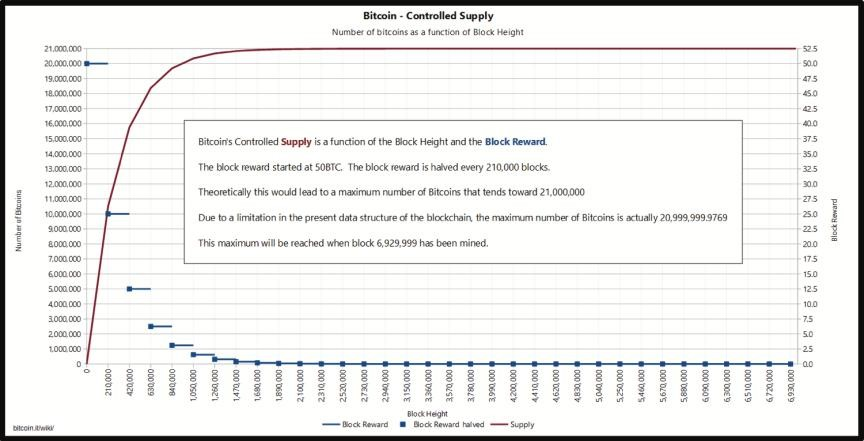
\includegraphics[width=10cm]{imagens/grafico-capitulo-05.jpg}
  \caption*{\url{https://en.bitcoin.it/w/images/en/4/42/Controlled_supply-supply_over_block_height.png}}
\end{figure}

Eventualmente, por volta do ano 2140, a Recompensa por Bloco desaparecerá totalmente, e os mineradores serão incentivados apenas pelas taxas pagas por aqueles que realizam as transações.

Esses números de emissão e de recompensa de bloco são aplicados no código Bitcoin - que, para reiterar, é totalmente de código aberto e pode ser validado por qualquer pessoa - dependendo de quão longe estamos na história do Bitcoin, produzindo um bloco que não siga essas regras fará com que você seja rejeitado por todos os outros que estão verificando as mesmas que estão escritas em seus códigos.

\section*{Controlando a Emissão e Intervalo de Mineração}


A mineração requer hardware e eletricidade, portanto, quanto mais hardware e eletricidade você controlar, maior será a probabilidade de encontrar o resultado mais rápido, em comparação às demais pessoas. Por exemplo, se houver 100 computadores com velocidade e custo energético igual na rede e você controlar 10 deles, encontrará o bloco vencedor em \textit{aproximadamente} 10\% das vezes. No entanto, a mineração é um processo baseado no acaso e na aleatoriedade, então é possível que horas ou mesmo dias possam se passar sem que você encontre um bloco.

Como foi falado na seção anterior, os mineradores não podem simplesmente conceder a si mesmos recompensas de blocos arbitrárias, ou seriam rejeitados pelos demais nodes. Mas e se eles gastarem muita energia para adiantar os blocos de mineração e colocarem as mãos em um monte de bitcoins, violando a restrição do projeto de que o cronograma de emissão deve ser conhecido com antecedência?

Vamos novamente ao exemplo de que há apenas 1000 hashes possíveis e nosso número de alvo sendo 100. Isso significa que 10\% das vezes vamos lançar um número menor que 100 e encontrar um bloco.

Digamos que leve 1 segundo para calcular cada hash. Se a cada segundo "lançarmos nosso dado" \  misturando as transações atuais e nosso nonce aleatório, e 10\% das vezes atingirmos um número menor que o alvo, então esperamos que leve cerca de 10 segundos, em média, para encontrar um hash válido.

O que acontece se dois computadores estiverem apostando nessa loteria? Eles têm duas vezes mais hashes sendo tentados, então esperamos que um hash válido seja encontrado em 5 segundos. E se 10 computadores estiverem jogando? Um deles encontrará um hash válido aproximadamente a cada segundo.

Isso cria um problema: se mais pessoas estão minerando, os blocos serão produzidos muito rapidamente. Isso gera dois resultados que não queremos:

\begin{enumerate}
\item Isso atrapalha a ideia de ter um cronograma de emissão pré-determinado. Queremos que seja emitido um número relativamente consistente de bitcoins por hora para ter certeza de que emitiremos todos eles até o ano 2140, e não antes disso;
\item Isso cria problemas de rede: se os blocos são extraídos tão rapidamente que não têm tempo de alcançar toda a rede antes que o próximo seja extraído, então não podemos chegar a um consenso sobre uma história linear de transações, uma vez que vários mineradores podem incluir a mesma transação em seus blocos, fazendo com que os blocos sejam inválidos por conterem transações que já foram gastas em outros blocos.
\end{enumerate}

E se menos pessoas estão minerando, criamos o problema oposto:

\begin{enumerate}
\item Os bitcoins estão sendo emitidos muito lentamente, novamente interferindo na emissão pré-determinada;
\item A blockchain pode se tornar inutilizável conforme as pessoas esperam horas, dias ou até mesmo semanas, para obter uma transação gravada no livro-razão.
\end{enumerate}


O número total de hashes por segundo executado por todos os mineradores da rede Bitcoin é conhecido como \textit{hash rate}.

\begin{figure}[htb]
  \centering
  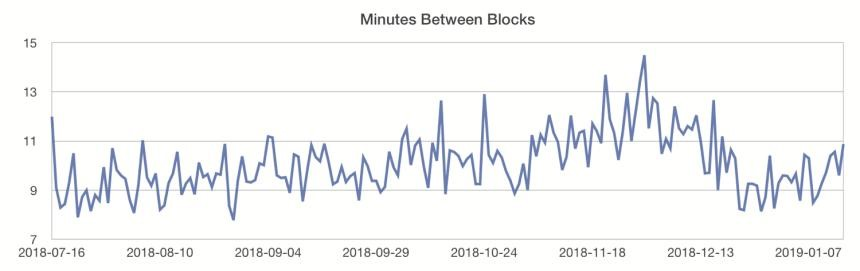
\includegraphics[width=10cm]{imagens/grafico2-capitulo-05.jpg}
  \caption*{\textit{Minutos entre blocos minerados}}
\end{figure}




\section*{Ajustes de dificuldade: concordando com o alvo}

%adicionado
Como Bitcoin é um sistema voluntario e sem permissão que pessoas podem participar quando desejarem, sem ninguém comandando, o numero de mineradores ativos em um dado momento pode variar drasticamente. Precisamos de uma maneira de manter a produção de blocos estável impedindo aumentos ou reduções no cronograma toda vez que um minerador novo entra na rede ou um minerador existente saia.

%da uma olhada na ultima frase do paragrafo a seguir Korea!!
%...if players leave the lottery, in order to keep the issuance and block times steady?

Como podemos tornar mais difícil encontrar hashes válidos se mais jogadores entrarem na loteria e mais fácil se os jogadores saírem dela, a fim de manter os tempos de emissão e de blocos estáveis?

%adicionado
Lembre que mineração de Bitcoin é uma loteria para tentar produzir um numero aleatório menor que um alvo.

\begin{figure}
  \centering
  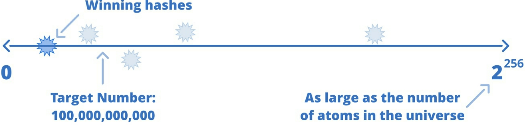
\includegraphics[width=10cm]{imagens/capitulo5/difficulty1.png}
  
  \caption*{\textit{Estamos tentando acertar esse pequeno espaço, o numero de possíveis resultados é grande, que irá demorar uma quantidade grande quantia de tempo para acerta la aleatoriamente.}}
\end{figure}

O Bitcoin resolve esse problema com um \textit{ajuste de dificuldade de mineração}. Como todos estão executando o mesmo código, que impõe as mesmas regras, e todos têm uma cópia de todo o histórico de blocos até este ponto, todos podem calcular de forma independente a rapidez com que os blocos estão sendo produzidos.

A cada 2016 blocos, o que leva aproximadamente o equivalente a duas semanas, olhamos para trás e descobrimos quanto tempo levou para produzir esses blocos e, em seguida, ajustamos nosso \textit{Número Alvo} para acelerar ou desacelerar a produção de blocos.

Todos os usuários pegam os últimos 2016 blocos e os dividem pelo tempo que levaram para produzir, criando assim uma média. Demorou mais de dez minutos? Estamos indo muito devagar. Demorou menos de dez minutos? Estamos indo rápido demais.

Agora podemos fazer um ajuste no \textit{Número Alvo} para que seja aumentado ou diminuído proporcionalmente a quanto mais rápido ou mais devagar queremos ir com base no intervalo de 10 minutos que está escrito no código fonte.

Podemos aumentar o \textit{Número Alvo} para um número mais alto, criando um espaço maior de hashes válidos, dando aos mineradores uma chance maior de encontrar um hash vencedor, gastando menos energia. Isso é chamado de \textit{redução da dificuldade}.
%faltou figura?

\begin{figure}
  \centering
  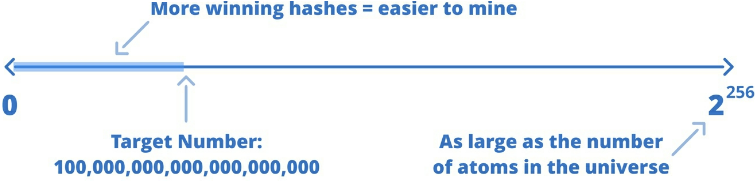
\includegraphics[width=10cm]{imagens/capitulo5/difficulty2.png}
  \caption*{\textit{Estamos tentando acertar esse pequeno espaço, o numero de possíveis resultados é grande, que irá demorar uma quantidade grande quantia de tempo para acerta la aleatoriamente.}}
\end{figure}

 De maneira contrária, podemos diminuir o \textit{Número Alvo} para que menos hashes sejam válidas e os mineradores tenham que gastar mais energia para encontrar um hash válido. Isso é chamado de \textit{aumento de dificuldade}.

Isso também significa que, para qualquer bloco, com base em quantos blocos vieram antes dele (a \textit{altura do bloco}), sabemos exatamente qual é o número alvo. Isso nos permite saber o limite mágico sob o qual o número do hash da Prova de Trabalho deve cair para um bilhete de loteria vencedor naquele bloco específico ser dado como válido.

O ajuste de dificuldade e numero alvo é possivelmente a inovação central do Bitcoin, permitindo a qualquer, independentemente, verificar o números da loteria baseados no alvo que eles podem independentemente calcular da mesma maneira que qualquer outra pessoa. É isso que permite a gente rodar uma loteria sem que ninguém nos diga a combinação vencedora.

%Esse paragrafo ta muito diferente do meu para ser o mesmo paragrafo logo defini ele como correto. 


%Isso é brilhante - não precisamos mais de um ente central para nos dizer nada. Tudo o que precisamos fazer é verificar por nós mesmos qual deve ser o Alvo e se a Prova de Trabalho reivindicada por um bilhete de loteria é um número vencedor que está abaixo dele.

O gráfico abaixo mostra a \textit{hash rate} como uma linha e a dificuldade como barras ao longo do tempo. A dificuldade parece uma escada porque é ajustada a cada 2016 blocos. Você pode ver que toda vez que a \textit{hash rate} sobe acima da dificuldade, a dificuldade aumenta para alcançar a \textit{hash rate}. Quando a \textit{hash rate} cai, como aconteceu entre outubro e dezembro de 2018, a dificuldade diminui. O ajuste de dificuldade sempre fica atrás do que quer que a \textit{hash rate} faça.

\begin{figure}
  \centering
  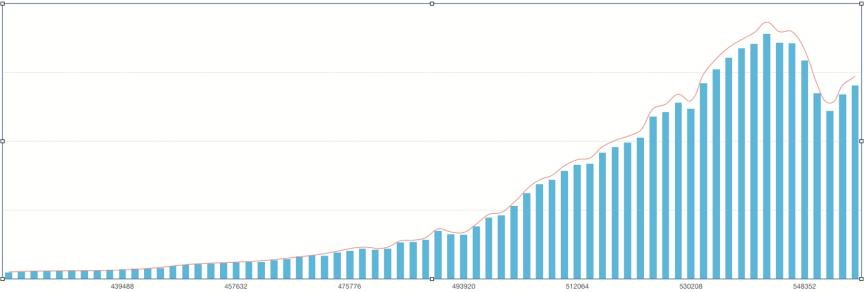
\includegraphics[width=10cm]{imagens/grafico3-capitulo-05.jpg}
  \caption{Hash Rate em relação a dificuldade}
\end{figure}

Como há uma defasagem de 2016 blocos entre os ajustes de dificuldade, é possível que haja picos massivos de aumento ou diminuição na \textit{hash rate} para mais ou menos produção de Bitcoin durante o período e isso pode violar levemente o cronograma da emissão.

%nao tem na minha versao

%Na verdade, estamos um pouco mais rápidos agora em comparação com a meta original de finalizar a emissão em 2140. 

Como adicionar \textit{hash rate} normalmente significa produzir uma grande quantidade de novo hardware, isso é relativamente incomum e não afeta muito as coisas, e esperamos que isso se mantenha assim no futuro.
%adicionado
As consequências de qualquer pico são limitadas a uma janela de 2016 blocos, no qual esses picos ocorreram, pois com o próximo ajuste de dificuldade voltaremos a media de 10 blocos por minuto.



\section*{Segurança e o valor em moeda fiduciária do Bitcoin}

Determinamos que o Bitcoin recalcula automaticamente a dificuldade com base no número de jogadores da loteria, ou seja, os mineradores consomem energia quando fazem o hash. É aqui que o mundo real começa a tocar nosso mundo digital. O preço do Bitcoin, o preço do hardware e da energia e o valor de dificuldade criam ciclos de feedback complexos:

\begin{enumerate}
%\item Os mineradores produzem bitcoin consumindo dinheiro para pagar a energia porque acham que as moedas terão algum valor;
\item Os especuladores compram bitcoin porque acham que ele está subindo, elevando o preço para R\$X;
\item Os mineiros gastam até R\$X de energia e hardware para tentar extrair um bitcoin;
\item Uma alta demanda dos compradores e um aumento no preço levam mais mineradores a minerar o bitcoin;
\item Mais mineradores significa mais energia consumida em bitcoin e a rede fica ainda mais segura, tranquilizando os compradores sobre a segurança do Bitcoin, às vezes levando a um ciclo de feedback que aumenta ainda mais o preço;
\item Após a passagem de 2016 blocos, a presença de mais mineradores e, portanto, maior quantidade de hash, causa um ajuste de dificuldade para cima;
\item Uma dificuldade maior significa um Número Alvo menor - os mineradores estão encontrando blocos com menos frequência - fazendo com que pelo menos alguns deles gastem mais R\$X em custos operacionais para extrair uma moeda;
\item Alguns mineradores se tornam não lucrativos, consumindo mais energia na mineração do que podem encontrar de bitcoin, fazendo com que rejeitem ser mineradores;
\item Outros 2016 blocos se passam. A dificuldade é recalculada para ficar mais fácil, já que alguns mineradores saíram do jogo;
\item Uma dificuldade menor significa que os mineiros que antes não eram lucrativos podem voltar a ficar online e fazer a mineração, ou novos mineiros podem entrar no jogo;
\item Vá para o item 1.
\end{enumerate}

Em um mercado em queda, o ciclo pode ir na outra direção, com os usuários vendendo as moedas, fazendo com que o preço caia e os mineiros se tornem não lucrativos.

%nao tem essa primeira frase na minha versao
%No entanto, ao contrário do que se pode ler na mídia sobre uma “espiral da morte”, 
O algoritmo de ajuste de dificuldade garante que sempre haverá algum tipo de equilíbrio entre o preço e o número de mineradores na rede. 
Mesmo que preços despenquem e acabem por remover metade do taxa de hash da rede, na próximo ajuste de dificuldade tornaria mineração lucrativo novamente em torno do novo equilíbrio de preços.

A natureza do ajuste de dificuldade é retirar os mineradores ineficientes em favor dos que operam com a energia mais barata possível. 
Ao longo do tempo, isso força mineradores de bitcoin a partes mais remotas do mundo onde recursos energéticos são abundantes. 
Uma reportagem da \textit{Coinshares} de 2019 estima que 75\% é feito com energias renováveis.

Na prática, nos últimos anos, o preço subiu rapidamente, assim como a taxa total de hash. Quanto mais alta a taxa de hash, mais difícil é atacar a rede porque, para controlar o que é gravado apenas no próximo bloco, é necessário ter muita energia e hardware sob seu controle, pois precisa ter mais da metade de toda a rede. Hoje, a energia utilizada pela rede de mineradores do Bitcoin é estimada como sendo maior do que um país de médio porte.




\section*{Taxas e o fim da recompensa de mineração} 

Se a recompensa de bloco vai eventualmente acabar, como vamos continuar incentivando mineradores a continuamente gastar energia para manter o livro-razão seguro?
A resposta do Bitcoin é taxas de transação financeira.
Não só eles substituem a recompensa de bloco mas incentivam o minerador a incluir transações nos blocos ao invés de minerar blocos vazios.

Taxas são determinadas pelo sistema de livre mercado onde usuários fazem lances para  utilizar o espaço escasso dentro de um bloco. Usuários que fazem transações indicam quanto querem pagar para os mineradores e os mineradores podem ou não incluir a transação que verem dependendo das taxas. 
Quando a poucas transações a serem incluídas nos blocos, taxas costumam cair, visto que não tem competição. Mas a medida que os espaços dentro dos blocos vão se preenchendo, usuários tendem a pagar mais  para que suas transações sejam concluídas rapidamente(dentro do próximo bloco). Aqueles que não querem pagar podem sempre ajustar suas taxas para valores mais baixos e esperar por mais tempo para que sua transação seja minerada quando tiver mais disponibilidade de espaço no bloco.

No sistema financeiro tradicional, taxas tendem a ser baseadas numa porcentagem da quantia a ser transicionada. Em Bitcoin o valor a ser transferido não impacta na taxa. Entretanto, taxas são proporcionais ao recurso escasso que elas consomem. Espaço no bloco. Taxas são mensuradas em satoshis por byte(8 bits) do espaço que consomem. Por tanto uma transação que envia milhões de bitcoins de uma pessoa para outra pode na pratica ser mais barata que uma transação que envia 1 bitcoin para dez recipiente, por conta de cada endereço necessitar de mais espaço no bloco.

No passado, houveram períodos em que o bitcoin estava com a demanda muito alta, tipo a \textit{bull run} do final de 2017. Nesse período as taxas estavam extremamente altas. Desde então novas funções foram implementadas para reduzir a pressão que as taxas causam na rede.

Uma dessas implementações se chama \textit{Segregated Witness}, que reorganiza como dados no bloco são representados. Transações que utilizam esse upgrade podem usar mais que 1MB de espaço através de uns truques que estão além do escopo desse livro.

Outro alivio às taxas vieram através de \textit{Batching}: exchanges,  outras baleias e outros jogadores de peso que participam do ecossistema começaram a combinar transações de Bitcoin para múltiplos usuários em uma única transação. Diferente do sistema tradicional de pagamentos do seus banco ou paypal que faz transações de uma pessoa a outra. Uma transação Bitcoin pode combinar um numero alto de entradas e gerar um numero alto de saídas. Então uma exchange que necessita enviar bitcoins para saque de 100 pessoas pode fazer isso em uma única transação. O que torna muito mais eficiente a utilização do espaço de bloco, um possível punhado de transações por segundos em algumas milhares de transações.

\textit{Segragated Witness} e \textit{Batching} já fizeram um bom trabalho em reduzir a demanda por espaço de bloco. Ainda haverá outras melhorias que estão na etapa de desenvolvimento para tornar o espaço no bloco mais eficiente. Mas de qualquer maneira, haverá outros momentos onde as taxas de transações de Bitcoin serão altas novamente devido a alta demanda por espaço de bloco.


Quase concluímos a invenção de todo o Bitcoin:

\begin{enumerate}
\item Substituiu um banco central por um livro-razão distribuído;
\item Instituiu um sistema de loteria para selecionar quem escreve no livro-razão;
\item Os participantes da loteria são forçados a consumir energia para comprar bilhetes por hash e torna mais fácil para todos poderem verificar os bilhetes vencedores, verificando os números hash produzidos pelos jogadores;
\item Diz aos jogadores da loteria que se eles não jogarem de acordo com as regras, rejeitamos os blocos, incluindo as \textit{transações de criação de moedas}, chamadas de \textit{coinbase}, para que eles não fossem pagos quando ganhassem, criando assim um desincentivo econômico para trapacear e um incentivo econômico para jogarem de acordo com as regras;
\item Controlou o tempo e a seleção do \textit{Alvo} para a loteria, permitindo que todos calculassem por si mesmos qual o \textit{Alvo} deveria ser, baseado nas regras codificadas e no histórico dos últimos 2016 blocos;
\item Aplicou o cronograma de emissão usando ajustes de dificuldade que são alterados de acordo com o aumento ou diminuição da \textit{hash rate};
\item Usou o código-fonte aberto para garantir que todos pudessem verificar por si mesmos se estavam aplicando as mesmas regras em relação à validade da transação, recompensa do bloco e cálculo de dificuldade.
\end{enumerate}

%isso esse paragrafo nao tem na minha versao(tirando a primeira e segunda frase(no qual mudei de posição)
% Qualquer um pode participar. Qualquer um pode jogar na loteria e criar bitcoins para si mesmo. Qualquer pessoa pode usar. A produção honesta de blocos é validada por toda a rede e recompensada com uma transação de \textit{coinbase} que paga ao minerador, ou punida por falta de recompensa e o minerador precisa consumir energia na mineração.
 
Não há mais entidade centralizada. Temos um sistema totalmente distribuído e descentralizado.
Quase temos a imagem completa do funcionamento da rede. Resta apenas um problema. Quando alguém se junta à rede e pede cópias do livro-razão, eles podem obter diferentes históricos de nodes diferentes. Como podemos impor uma história única e linear e como podemos evitar que os mineradores reescrevam o passado?




\part{Mantendo Suas Moedas Seguras}
\label{ch:capitulo6}
\chapter*{Mantendo Suas Moedas Seguras}

Até agora, falamos como gerenciamos e mantemos as cópias e gravamos no livro razão distribuído sem que possa haver coerção ou corrupção. Mas o que acontece quando um ganhador da loteria quer ser malicioso? Ganhar o direito de escrever em livro-razão significa que eles podem alterar lançamentos históricos no livro-razão? Evandro, Danilo e Fernanda podem conspirar para reescrever a história ou alterar os saldos das contas e dar a si mesmos moedas extras?

Vamos entrar na blockchain. Um termo de marketing que permeou grande parte do setor de tecnologia, a blockchain nada mais é do que a ideia de que os blocos do Bitcoin são encadeados para fornecer links de um conjunto de transações para o próximo bloco.

Mentimos um pouco no capítulo anterior para manter as coisas mais simples. Quando você minera jogando na loteria de Prova de Trabalho, você não está apenas fazendo o hash das transações que querem ir para o próximo bloco junto com o nonce. Na verdade, você também está fornecendo o hash do último bloco como entrada em sua função hash, vinculando assim seu bloco ao bloco anterior.

Isso nos permite construir um registro histórico de cada bloco desde o Bloco Gênesis (primeiro bloco do Bitcoin) extraído por Satoshi. Quando escrevemos um novo bloco na blockchain, temos que validar que este bloco não contém nenhuma transação que gaste bitcoins que já foram gastos em blocos anteriores.

\newpage

\begin{figure}
  \centering
  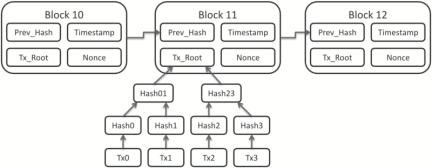
\includegraphics[width=10cm]{imagens/capitulo-06-bloco.jpg}
  \caption{\url{https://upload.wikimedia.org/wikipedia/commons/7/7a/Bitcoin_Block_Data.png}}
\end{figure}

Lembre-se de que a saída de uma função hash é aleatória e dependente de todos os dados de entrada que nela constam. Agora modificamos nossos hashes do bloco para incluir três entradas diferentes:

\begin{samepage}
\begin{enumerate}
\item As transações que queremos incluir no livro-razão;
\item Um nonce aleatório;
\item O hash do bloco anterior que estamos usando como sendo a base do histórico do livro-razão.
\end{enumerate}
\end{samepage}

Se alguma dessas três coisas forem alteradas, o hash de saída mudará de maneira imprevisível. Esse comportamento cria uma propriedade interessante: se você adulterar os dados de qualquer bloco antigo, alterará seu hash. Se você alterar o hash de qualquer bloco antigo, alterará o hash de cada bloco que vier depois.

Isso torna a corrente inviolável. Se alguém tentasse alterar um bloco mais antigo na cadeia, teria que recalcular o hash de Prova de Trabalho do bloco que está adulterando e de cada novo bloco que vier depois.

Efetivamente, cada novo bloco extraído no Bitcoin aumenta a segurança dos blocos que vieram antes dele. Uma transação em um bloco que possui 6 blocos posteriores a ele é considerada definitivamente inalterada. Seria necessária uma enorme quantidade de energia para recalcular os últimos seis blocos na taxa de hash total atual. Alterar um bloco a 100 blocos atrás? Nem pense nisso, esquece.

É importante entender que não há finalidade real de transação no Bitcoin. Cada comerciante ou processador de pagamentos decide por si mesmo o que considera final. Hoje, a maioria das pessoas aceita 6 confirmações - seis blocos extraídos depois daquele que contém a transação - como sendo definitivo, mas os comerciantes podem definir isso como quiserem.

Se você está vendendo um livro digital que tem custo marginal para você como comerciante, pode querer apenas 1 confirmação, ou mesmo zero confirmações, entregando o bem digital assim que vir a transmissão da transação na rede. Se você está vendendo uma casa, talvez queira esperar por doze confirmações, ou cerca de duas horas de mineração. Quanto mais você espera, mais Provas de Trabalho são empilhadas no topo do bloco que contém suas transações e mais caro se torna no mundo real para reverter a transação.

Se a taxa de hash do Bitcoin cair significativamente, o que significa que menos energia está protegendo cada bloco, pode-se sempre aumentar o número de confirmações necessárias para a liquidação final. Embora isso possa parecer muito complicado no início, é importante ter em mente que as transações com cartão de crédito normalmente podem ser revertidas 120 dias após serem feitas. Por outro lado, o Bitcoin é um dinheiro de liquidação final que não pode ser retirado de você, como dinheiro ou ouro. Deste ponto de vista, a reversibilidade e a finalidade das transações no Bitcoin é, na verdade, uma grande melhoria em relação à maioria das redes de pagamento tradicionais.

Vamos voltar ao nosso exemplo do Capítulo 3, onde Henrique se junta a uma rede e obtém diferentes cópias do livro-razão. O livro-razão que ele pegou da Carol é honesto, mas os livros-razão do Evandro, Danilo e Fernanda são maliciosos, onde eles excluíram um bloco antigo que continha os gastos originais da Alice para que eles pudessem enganar Henrique fazendo-o pensar que ela ainda tinha suas moedas. Antes de vincular os blocos entre si por Prova de Trabalho, Henrique não sabia que um bloco antigo foi excluído.

Como cada bloco contém uma Prova de Trabalho, ele sabe aproximadamente quanta energia foi consumida para produzi-lo com base no Número Alvo. Como cada bloco aponta para um bloco anterior, ele sabe que para alterar o histórico de um bloco antigo seria necessário recalcular a Prova de Trabalho não apenas do bloco adulterado, mas de cada bloco que veio depois dele. Como ele pode ver todas as transações em cada bloco, ele pode garantir que nenhum gasto duplo foi feito.

\begin{figure}
  \centering
  
\includegraphics[width=5cm]{imagens/capitulo-06-mineracao.jpg}
  \caption{Ao contrário da mineração de ouro, que também consome energia, o processo de mineração de Bitcoin na verdade protege a rede para tornar o livro-razão à prova de adulteração.}
\end{figure}

\paragraph{E se duas pessoas encontrarem um bloqueio ao mesmo tempo?}
\paragraph{}

Falta uma peça no sistema de consenso. Imagine que agora estamos administrando uma rede mundial. Pessoas em todo o mundo, dos Brasil ao Japão, estão conectadas a essa rede global e todas estão jogando na loteria da Prova de Trabalho.

Alguém em São Paulo encontra um bloco válido. Eles o anunciam na rede e todos os computadores do Brasil começam a detectá-lo. Enquanto isso, alguém em Tókio também encontra um bloco a poucos segundos depois do bloco de São Paulo. Seus vizinhos ainda não ouviram falar do bloco brasileiro, então eles ficam sabendo primeiramente do bloco japonês.

Como os dois blocos se propagam através dos nodes vizinhos na rede, agora temos duas versões concorrentes da blockchain. Os brasileiros têm um que tem o bloco brasileiro no final, e os japoneses têm o seu próprio bloco. A rede está dividida por não saber qual a blockchain é a cópia correta do livro-razão, uma vez que ambos contêm quantidades equivalentes de Prova de Trabalho e ambos contêm transações válidas.

Você não pode contar com nenhum ente central para lhe dizer qual deles é o verdadeiro. O que você faz? O Bitcoin fornece uma solução bem simples para este problema: vamos apenas esperar para ver o que acontece. Existem agora duas versões concorrentes da blockchain. No próximo período de aproximadamente dez minutos, outro bloco será minerado. Os brasileiros estarão minerando no topo do bloco de que ouviram falar pela primeira vez, e os japoneses estarão minerando no topo de seu bloco.

Qualquer que seja o lado que minere primeiro, será o escolhido como sendo o verdadeiro. Como? Porque no código do Bitcoin há uma regra que diz que a cadeia de Prova de Trabalho Cumulativa Mais Longa resolve qualquer divisão que ocorra na cadeia. Quem consome mais energia vence. A regra de resolução de inconsistências entre cadeias com base em sua Prova de Trabalho cumulativa total agora é chamada de Consenso de Nakamoto, em homenagem a Satoshi Nakamoto.

Digamos que os japoneses minerem o próximo bloco. A rede deles está agora um bloco à frente da brasileira. Quando eles divulgarem essa descoberta, os nodes brasileiros do Bitcoin reconhecerão que os nodes japoneses produziram uma cadeia de Prova de Trabalho cumulativa mais longa e se reorganizarão (ou farão o que chamamos de “reorg”). Isso significa que eles vão jogar fora o bloco que mineraram em favor dos japoneses porque a blockchain deles é maior. O bloco brasileiro agora é chamado de \textit{órfão}. Uma vez que foi rejeitado, significa que o minerador que o encontrou não foi recompensado.

Você pode notar que, embora tenha me referido aos nodes como brasileiros e japoneses, na realidade os nodes não sabem nada sobre a identidade uns dos outros, localização geográfica e assim por diante. A única prova de validade de que precisam é que alguém tenha a cadeia de Prova de Trabalho Cumulativa Mais Longa e que as transações na cadeia sejam todas válidas (sem gastos duplos, etc.).

A probabilidade de ocorrer essa divisão da cadeia é muito baixa - costumava acontecer uma vez por mês ou menos, mas recentemente não aconteceu muito devido a melhorias na tecnologia de propagação de bloco e conectividade de rede entre os mineradores.

Parte da razão pela qual o Bitcoin produz blocos relativamente pequenos aproximadamente a cada dez minutos é para garantir que os blocos órfãos sejam extremamente raros. A outra razão é manter os requisitos de hardware para executar um node relativamente baixos para encorajar mais nodes no sistema.

Se nós produzíssemos blocos a cada segundo ou tivéssemos blocos muito grandes, teríamos uma probabilidade muito alta de que os blocos brasileiros e japoneses entrariam em conflito porque eles estão geograficamente distantes e levam mais tempo para se alcançarem. Se os órfãos acontecessem com muita frequência, a cadeia de blocos se desfaria porque haveria órfãos em órfãos e os nodes não seriam capazes de concordar sobre um histórico linear de transações.

Um node do Bitcoin precisa apenas se conectar a um outro node honesto que tenha o blockchain mais recente na rede para evitar ser enganado por invasores que podem fornecer informações falsas. Os nodes constantemente conversam uns com os outros para garantir que tenham os blocos mais recentes. Se o seu node quiser saber qual cópia da blockchain é verdadeira, ele só precisa procurar a cadeia com a Prova de Trabalho mais cumulativa. Como todos os outros também estão seguindo esta regra, codificada no software, isso garante que haja consenso sobre qual é o verdadeiro estado do livro-razão.

É extremamente difícil, portanto, para hackers mal-intencionados fornecer a um nó uma cópia falsa do blockchain, pois isso exigiria cortar a conexão desse nó com qualquer outro nó honesto e conectá-lo apenas a nós malignos.

Embora o fork normalmente aconteça devido ao acaso e atrasos de propagação de blocos, ao invés de ser motivado maliciosamente, também é possível que uma entidade sem boas intenções que deseja controlar o que vai para o próximo bloco possa tirar vantagem do Consenso de Nakamoto, controlando mais de 50\% do total do hash da rede e produzindo a mais longa cadeia de Prova de Trabalho Cumulativa. Discutiremos os detalhes desse caso, chamado de "ataque de 51\%", no Capítulo 9.

\paragraph{Segurança e o valor em moeda fiduciária do Bitcoin}
\paragraph{}

Determinamos que o Bitcoin recalcula automaticamente a dificuldade com base no número de jogadores da loteria, ou seja, os mineradores consomem energia quando fazem o hash. É aqui que o mundo real começa a tocar nosso mundo digital. O preço do Bitcoin, o preço do hardware e da energia e o valor de dificuldade criam ciclos de feedback complexos:

\begin{enumerate}
\item Os mineradores produzem bitcoin consumindo dinheiro para pagar a energia porque acham que as moedas terão algum valor;
\item Os especuladores compram bitcoin porque acham que ele está subindo, elevando o preço para R\$X,xx;
\item Os mineiros gastam até R\$X,xx de energia e hardware para tentar extrair um bitcoin;
\item Uma alta demanda dos compradores e um aumento no preço levam mais mineradores a minerar o bitcoin;
\item Mais mineradores significa mais energia consumida em bitcoin e a rede fica ainda mais segura, tranquilizando os compradores sobre a segurança do Bitcoin, às vezes levando a um ciclo de feedback que aumenta ainda mais o preço;
\item Após a passagem de 2016 blocos, a presença de mais mineradores e, portanto, maior quantidade de hash, causa um ajuste de dificuldade para cima;
\item Uma dificuldade maior significa um Número Alvo menor - os mineradores estão encontrando blocos com menos frequência - fazendo com que pelo menos alguns deles gastem mais R\$X,xx em custos operacionais para extrair uma moeda;
\item Alguns mineradores se tornam não lucrativos, consumindo mais energia na mineração do que podem encontrar de bitcoin, fazendo com que rejeitem ser mineradores;
\item Outros 2016 blocos se passam. A dificuldade é recalculada para ficar mais fácil, já que alguns mineradores saíram do jogo;
\item Uma dificuldade menor significa que os mineiros que antes não eram lucrativos podem voltar a ficar online e fazer a mineração, ou novos mineiros podem entrar no jogo;
\item Vá para o item 1.
\end{enumerate}

Em um mercado em queda, o ciclo pode ir na outra direção, com os usuários vendendo as moedas, fazendo com que o preço caia e os mineiros se tornem não lucrativos. No entanto, ao contrário do que se pode ler na mídia sobre uma “espiral da morte”, o algoritmo de ajuste de dificuldade garante que sempre haverá algum tipo de equilíbrio entre o preço e o número de mineradores na rede. Também retira os mineradores ineficientes em favor dos que operam com a energia mais barata possível.

Na prática, nos últimos anos, o preço subiu muito rapidamente, assim como a taxa total de hash. Quanto mais alta a taxa de hash, mais difícil é atacar a rede porque, para controlar o que é gravado apenas no próximo bloco, é necessário ter muita energia e hardware sob seu controle, pois precisa ter mais da metade de toda a rede. Hoje, a energia utilizada pela rede de mineradores do Bitcoin é estimada como sendo maior do que um país de médio porte.
\part{Contas Sem Identidade}
\label{ch:capitulo7}
\chapter*{Contas Sem Identidade}

Até agora, construímos um livro-razão distribuído sem autoridade central, um sistema de loteria para selecionar quem escreve, um sistema para recompensar bons mineradores e punir os que se comportam mal, uma forma de ajustar a dificuldade de mineração para garantir um cronograma de cunhagem consistente e reduzir conflitos, e um sistema para verificar a validade da cadeia, examinando a prova cumulativa de trabalho e o histórico de transações.

Agora vamos lidar com a identidade. Em um sistema bancário tradicional, você envia dinheiro identificando-se ao banco, seja por meio da apresentação de um código ou PIN pessoal ou da apresentação do nome de usuário e senha, no aplicativo. O banco garante que duas pessoas não compartilhem uma só identidade.

Já que agora não temos uma entidade central para rastrear os indivíduos, como podemos abrir contas em nosso novo sistema financeiro baseado em Bitcoin e como podemos garantir que, quando Ana anunciar que deseja pagar Bruno, seja realmente ela e, tenha a autoridade de enviar esses fundos?

\paragraph{Gerando uma “Conta Bitcoin”}
\paragraph{}

Já que não podemos contar com um intermediário central como um banco para manter um registro de todas as contas, e como as pessoas podem entrar e sair quando quiserem, sem permissão, como podemos gerenciar suas contas?

E se permitirmos que todos registrem seu próprio nome de usuário e senha? Um banco normalmente verifica se um nome de usuário ainda não está em uso, mas isso não é possível neste caso, já que não temos um ator central distribuindo identidades. Portanto, precisamos de algo maior, mais forte e mais exclusivo do que um nome de usuário e uma senha. Esta técnica deve ser semelhante aos capítulos anteriores. Mais uma vez, precisamos de um número aleatório gigante.

Assim como possibilitamos que todos comprassem bilhetes de loteria gerando grandes números aleatórios, podemos usar o mesmo truque para gerar contas. Para criar uma “Conta Bitcoin”, também conhecida como endereço, primeiro geraremos um par de números de 256 bits matematicamente vinculados, conhecido como \textit{par de chaves pública/privada}. Novamente, \(2^{256}\) é tão grande quanto o número de átomos no universo, então duas pessoas gerando acidentalmente o mesmo par de chaves é quase impossível.

O par de chaves tem algumas propriedades interessantes. Você pode usar qualquer uma das chaves para criptografar uma mensagem e a outra para descriptografá-la. Além disso, você está convidado a compartilhar sua chave pública com o mundo inteiro. Saber essa chave não permite que eles tenham acesso à sua chave privada.

Vamos dar uma olhada qual o processo que Ana faz para enviar as moedas para Bruno. Para receber uma transação, Bruno gera um par de chaves privadas/públicas e mantém sua chave privada em segredo. Ele produz um \textit{endereço}, um grande número com base em sua chave pública. Bruno, então, compartilha esse número de endereço com Ana para que ela possa enviar moedas para ele.

Ana agora precisa informar à rede que está enviando moedas para o endereço público de Bruno à partir de seu próprio endereço público. Como ela prova que está autorizada a gastar naquele endereço público? Ela faz isso fornecendo prova de que possui a chave privada desse endereço, mas sem realmente revelar sua chave privada.

Essa prova é chamada de \textit{assinatura digital}. Ana constrói uma transação, que essencialmente é apenas um pedaço de dados que parece algo como “o endereço 12345 está enviando 2 bitcoins para o endereço 56789”, exceto que os números do endereço são, na verdade, números gigantes. Ela então faz o hash de sua transação e criptografa o hash com sua chave privada, criando uma assinatura digital.

Quando ela publica sua transação na rede, ela revela sua chave pública (de onde ela está enviando). Uma vez que todos possuem a chave pública, todos podem facilmente descriptografar a assinatura digital. Mas eles só seriam capazes de descriptografar se fosse, de fato, criptografado com a chave privada correspondente que apenas Ana conhece.

Portanto, apenas a virtude de ser capaz de descriptografar corretamente a assinatura permite que todos saibam que Ana tem a chave privada para aquele endereço, sem realmente revelar sua chave privada.

Quando você move dinheiro em um banco, você fornece a eles seu nome de usuário e senha. Quando você passa cheques, assina seu nome para autenticar que é você quem está escrevendo o cheque. Ao mover o bitcoin, você prova que possui a chave do endereço que contém o bitcoin.

Ao contrário de uma assinatura em um cheque ou de sua senha de banco, sua assinatura digital é específica para os dados de transação exclusivos que você está assinando. Portanto, não pode ser roubada e reutilizada em uma transação diferente. Cada transação recebe uma assinatura diferente, mesmo que seja baseada na mesma chave privada.
\newpage
\paragraph{Você consegue adivinhar uma chave privada?}
\paragraph{}

Vamos descobrir as chances de adivinhar uma chave privada, o que lhe daria a capacidade de mover as moedas no endereço público correspondente. Lembre-se de que uma chave é composta por 256 bits. Cada bit possui apenas dois valores (um ou zero). Isso significa que você pode visualizar cada bit como um cara ou coroa.

Se tivéssemos uma chave privada de 1 bit, seria como jogar uma moeda. Cara ou coroa, um ou zero? Você tem uma chance em duas de acertar.

Revisão rápida de probabilidade básica: A probabilidade de ocorrência de vários eventos é calculada multiplicando-se a probabilidade individual de cada evento. Se um lançamento de moeda tem 1/2 chance de dar cara, então a chance de dois lançamentos de moeda consecutivos dar cara é 1/2 x 1/2 = 1/4 ou 1 em 4.

Se tivéssemos 2 bits, seriam dois lançamentos de moeda consecutivos. \(2^2\) = 4, então você tem uma chance em 4.

Se você adivinhasse o resultado de 8 lançamentos consecutivos de moeda, seria \(2^8\), ou uma chance em 256.

Uma placa de carro americana tem 6 letras e números. Existem 26 letras e 10 números, portanto, um total de 36 caracteres. Como há seis deles, o número de placas de carros possíveis = \(36^6\), então suas chances de adivinhar a minha são de uma em 2.176.782.336 (uma em dois bilhões)\footnote{A inspiração para esta seção veio de uma excelente postagem no Medium que detalha as probabilidades de uma variedade de eventos. Recomendo a leitura da postagem completa para contexto: \url{https://medium.com/breathe-publication/a-dance-with-infinity-980bd8e9a781}}.

Um cartão de crédito tem dezesseis dígitos. Cada dígito pode ter 10 valores, e há 16 deles, então suas chances de adivinhar meu cartão de crédito são de uma em \(10^{16}\), que é uma em 10.000.000.000.000.000.000 ou aproximadamente uma em dez quintilhões.

Existem cerca de \(10^{50}\) átomos na Terra. Se estou pensando em um ao acaso, suas chances de adivinhar exatamente qual átomo, é de:

\begin{samepage}
\begin{quote}{Um em 1.000.000.000.000.000.000.000.000.000.000.\newline
000.000.000.000.000.000.000.}\end{quote}
\end{samepage}

Uma chave privada tem 256 bits, que é \(2^{256}\) ou cerca de \(10^{77}\). Na verdade, está mais perto em magnitude de adivinhar um átomo específico de todo o universo ou de ganhar na Mega Sena 9 vezes seguidas usando apenas 6 números:

\begin{samepage}
\begin{quote}{Uma chance em 115.792.089.237.316.195.423.570.985.\newline 008.687.907.853.269.984.665.640.564.039.457.584.007.\newline
913.129.639.936}\end{quote}
\end{samepage}

Mas e se você tivesse um computador superpoderoso para fazer as suposições? Não posso fazer mais justiça a este assunto do que a este post\footnote{A postagem completa do Reddit que descreve como adivinhar uma chave de 256 bits está disponível aqui: \url{https://bit.ly/2Dbw9Qd}} do Reddit, que recomendo a leitura na íntegra. Embora seja técnico, o parágrafo final dá uma boa ideia do que seria necessário para listar todas as chaves de 256 bits possíveis:

\begin{quotation}\begin{samepage}
\enquote{Então, se você pudesse usar o planeta inteiro como um disco rígido, armazenando 1 byte por átomo, usando estrelas como combustível e percorrendo 1 trilhão de chaves por segundo, você precisaria de 37 octilhões de Terras para armazená-lo e 237 bilhões de sóis para alimentar o dispositivo capaz de fazer isso, o que levaria 3,6717 octodecilhões de anos.}
\begin{flushright} -- U/PSBLAKE EM R/BITCOIN
\end{flushright}\end{samepage}\end{quotation}

Basicamente, é impossível adivinhar a chave privada de alguém. Não apenas isso, mas o número de endereços de Bitcoin é tão grande que as melhores práticas realmente exigem a geração de um novo endereço para cada transação que você fizer. Então, em vez de ter uma conta bancária, você pode ter milhares ou até milhões de contas Bitcoin, uma para cada transação que já recebeu.

Pode ser desconcertante que sua conta Bitcoin seja protegida apenas por acaso, mas espero que a ilustração acima dê a você uma ideia de que isso é muito mais seguro do que a senha de sua conta bancária, armazenada em um servidor centralizado, disponível para hackers.

\paragraph{Rastreamento de saldos}
\paragraph{}

É hora de corrigir uma última mentira inofensiva que já dissemos em capítulos anteriores. Na verdade, não há saldos mantidos no livro-razão. O Bitcoin usa um modelo chamado UTXO: Unspent Transaction Outputs.

A ideia do UTXO é que cada transação é um conjunto de entradas que são consumidas para produzir novas saídas. Pense nisso como enviar um monte de moedas para uma máquina que derrete e cunha novas moedas de qualquer valor que quisermos. Um UTXO é simplesmente a palavra para uma saída de transação - uma moeda produzida por uma transação anterior, incluindo uma \textit{transação do tipo coinbase} de recompensa em bloco - que ainda não foi gasta em outro endereço.

Digamos que Ana tenha um endereço que contém 1 bitcoin. Ela deseja enviar 0,3 bitcoins para Bruno. Ela gera uma transação que mostra seu endereço com 1 bitcoin com o seu UTXO como entrada e duas saídas: um novo endereço bitcoin UTXO que vale 0,3 como saída para o endereço do Bruno e um novo UTXO que vale 0,7 como saída para seu próprio endereço como troco. O troco pode ir para o endereço de envio original ou, para melhor privacidade, ela pode enviá-la para um novo endereço que foi gerado instantaneamente.

Já que não há nenhuma maneira de dizer quem controla qual endereço na blockchain (para isso, você precisa saber as chaves privadas correspondentes e vinculá-las às identidades do mundo real), o modelo UTXO permite um mecanismo de privacidade muito bom, permitindo a criação de novos endereços sempre que as moedas são movidas.

Assim, para verificar o “saldo” de um determinado endereço, na verdade temos que somar todos os UTXOs que possuem este endereço como saída. O conjunto total de UTXOs atuais no Bitcoin aumenta quando as pessoas enviam de um endereço para vários e diminui quando as pessoas realizam transações de “consolidação” em que moedas de vários endereços são gastas em um endereço.

O modelo UTXO permite a validação fácil e eficiente de gastos duplos, uma vez que qualquer UTXO em particular só pode ser gasto uma vez. Não precisamos saber todo o histórico de gastos de uma conta específica.

Também podemos criar e destruir qualquer número de UTXOs de uma vez, criando transações complexas que misturam diferentes entradas e saídas. Isso permite a ideia de “mistura de moedas”, em que várias partes participam de uma única transação de Bitcoin que mistura qualquer número de entradas para produzir qualquer número de saídas, obscurecendo assim o histórico dos UTXOs. Ele também permite que as pessoas consolidem moedas de vários endereços para um ou espalhem-nas entre vários endereços para melhorar a segurança e a privacidade.
\newpage
\paragraph{Carteiras}
\paragraph{}

Como gerar uma conta nada mais é do que gerar um número aleatório de 256 bits para ser sua chave privada, e podemos criar milhares ou milhões de contas, precisamos de um mecanismo para rastreá-las. No Bitcoin, a palavra \textit{carteira} é usada para se referir a qualquer tipo de dispositivo que rastreia suas chaves. Pode ser tão simples como um pedaço de papel ou tão complexo como uma peça de hardware.

O software original do Bitcoin publicado por Satoshi veio com uma carteira de software. Essa carteira geraria seu par de chave pública/privada (lembre-se novamente de que a chave pública é usada para criar seu endereço Bitcoin e sua chave privada permite que você assine transações para gastar moedas desse endereço).

Ao contrário da carteira do seu banco, que normalmente tem a forma de um único aplicativo móvel ou internet banking, o Bitcoin é um sistema completamente aberto. Portanto, existem centenas de carteiras, a maioria das quais é gratuita, sendo muitas delas também de código aberto, bem como meia dúzia de implementações de carteiras de hardware, com outras sendo produzidas. Qualquer pessoa com conhecimento de programação de computadores pode construir sua própria carteira ou ler o código de uma carteira de código aberto para garantir que nada de suspeito esteja acontecendo. Este é outro lugar no Bitcoin onde a inovação sem permissão está acontecendo em um ritmo rápido, ao contrário do aplicativo móvel do seu banco.

Visto que sua chave privada é a única coisa de que você precisa para gastar suas moedas, você deve guardá-la bem. Se alguém roubar seu cartão de crédito, você pode ligar para a empresa e registrar uma reclamação de fraude e tentar obter seu dinheiro de volta. No Bitcoin, não há intermediário. Se alguém tem sua chave privada, eles controlam suas moedas e não há ninguém que você possa ligar.

As chaves privadas também são altamente suscetíveis a perdas. Se você armazenar sua carteira no computador e ele for roubado ou pegar fogo, você tem um problema. Se você seguir as práticas recomendadas do Bitcoin para gerar um novo endereço toda vez que receber um pagamento, armazenar e fazer backup com segurança dessas chaves privadas se tornará algo muito custoso.

Com o tempo, o ecossistema Bitcoin desenvolveu uma série de soluções para esse problema. Em 2012, o BIP32 (Bitcoin Improvement Proposals ou Proposta de Melhoria do Bitcoin, um mecanismo para as pessoas espalharem ideias sobre como melhorar o Bitcoin) foi arquivado com a proposta de criar Carteiras Determinísticas Hierárquicas. A ideia por trás disso é que usando apenas um único número aleatório (seed), podemos gerar uma cadeia inteira de pares de chaves públicas/privadas: endereços de Bitcoin e chaves de assinatura para eles.

Hoje em dia, se você usar qualquer um dos softwares comumente disponíveis ou carteiras de hardware, eles gerarão automaticamente novas chaves para você para cada transação e permitirão que você faça backup de apenas uma única seed.

Em 2013, o BIP39 veio para tornar o backup de chaves ainda mais fácil. Em vez de usar um número completamente aleatório, as chaves seriam geradas a partir de um conjunto aleatório de palavras que seriam legíveis por seres humanos. Aqui está um exemplo de seed:

\begin{samepage}
\begin{quote}{witch collapse practice feed shame open despair creek road again ice least}\end{quote}
\end{samepage}

Com esse método, o backup das chaves se tornou muito fácil: você pode escrever a seed em um pedaço de papel e colocá-la em um cofre. Você pode até memorizar a frase e sair de um regime econômico decadente como a Venezuela, sem que ninguém saiba que você está carregando sua riqueza na cabeça.

Além disso, um endereço Bitcoin pode exigir mais de uma chave privada para ser acessado. Endereços multisignature ou \textit{multisig} podem empregar uma grande variedade de esquemas de segurança. Por exemplo, duas pessoas podem compartilhar uma conta usando multisig 1 de 2, onde qualquer uma das partes pode assinar as transações, ou um multisig 2 de 2, que exige que ambas as partes forneçam as chaves privadas para gastar.

Você pode fazer um sistema de depósito simples usando um multisig 2 de 3. O comprador obtém uma chave, o vendedor obtém outra chave e uma terceira chave é dada a um verificador. Se o comprador e o vendedor concordarem, eles podem desbloquear os fundos sem a necessidade do verificador.

Em caso de litígio, o verificador pode agir em conjunto com uma das partes para desbloquear os fundos.

Você pode usar um esquema multisig 3 de 5 para se proteger contra a perda de chaves, permitindo-se perder até 2 das 5 chaves e ainda ser capaz de desbloquear a conta. Você pode armazenar duas das chaves em lugares diferentes, duas com amigos de confiança diferentes que não se conhecem e uma com um serviço de custódia especializado como o BitGo que assina suas transações, tornando seu Bitcoin muito difícil de ser roubado enquanto se protege das perdas das chaves.

Você pode ir ainda mais longe e criar endereços que são desbloqueados por condições bastante complexas, como conhecimento de números secretos ou ficar bloqueado por um período específico de tempo. Você pode, por exemplo, fazer um endereço de bitcoin do qual você não pode gastar por 10 anos, não importa o quanto alguém queira forçá-lo a mudá-lo.

Isso é profundo e transforma o mundo. Nunca antes foi possível transportar seus bens de uma forma completamente segura contra apreensão ou roubo.
%\part{O Bitcoin Client}
\chapter{Quem faz as regras?}
\label{ch:capitulo8}

Agora temos um sistema distribuído funcional para acompanhar e transferir valor.
Vamos revisar o que criamos até agora:

\begin{samepage}
\begin{enumerate}
\item Um livro-razão distribuído, uma cópia que é mantida por todos os participantes;
\item Um sistema de loteria baseado em Prova de Trabalho e ajustes de dificuldade para manter a rede segura e o cronograma de emissão consistente;
\item Um sistema de consenso que garante que cada participante possa validar todo o histórico da blockchain para si, usando um software de código aberto chamado Bitcoin Client;
\item Um sistema de identidade usando assinaturas digitais que permite a criação arbitrária de caixas de correio semelhantes a contas que podem receber bitcoins sem uma autoridade central.
\end{enumerate}
\end{samepage}

Agora é hora de enfrentar uma das coisas mais interessantes e contra-intuitivas do Bitcoin: De onde vêm as regras, como são aplicadas e como elas podem ser modificado ao longo do tempo.

\section*{O software do Bitcoin}


Ao longo dos capítulos anteriores, presumimos que todos na rede estavam validando as mesmas regras: ou seja, estão rejeitando gastos duplos, garantindo que cada bloco contenha a quantidade adequada de Prova de Trabalho, que cada bloco aponte para o bloco anterior da blockchain atual e que cada transação contida no bloco esta devidamente assinada pelo proprietário daquele endereço, entre um monte de outras coisas com as quais as pessoas concordaram ao longo do tempo.

Também dissemos que o Bitcoin é um software de código aberto. 
O código aberto significa que qualquer pessoa pode ler seu código e também que qualquer pessoa pode atualizar sua própria cópia com o código que quiser. 
Como as mudanças chegam ao Bitcoin?

O Bitcoin é um \textit{protocolo}.
Em software de computador, este termo se refere a um conjunto de regras que o software segue.
No entanto, contanto que você siga o conjunto de regras que todos estão seguindo, você é livre para modificar seu software como desejar.
Quando dizemos que as pessoas “executam nodes de Bitcoin”, o que realmente queremos dizer é que elas executam um software que se comunica usando o protocolo Bitcoin.
Este software pode conversar com outros nodes Bitcoin, transmitir transações e blocos para eles, descobrir outros nodes para fazer se conectar e assim por diante.

Os detalhes reais de como o software é implementado dependem de qualquer pessoa que o execute.
Na verdade, existem muitas implementações do protocolo Bitcoin.
O mais popular deles é chamado Bitcoin Core e é a extensão do trabalho lançado pela primeira vez por Satoshi Nakamoto.

Existem outros clientes também, alguns até mesmo escritos em outras linguagens de computador e mantidos por pessoas diferentes. 
Como o consenso em Bitcoin é crítico, o que significa que todos os nodes devem concordar sobre quais blocos são ou não válidos, a grande maioria dos nodes executa o mesmo software (Bitcoin Core) para evitar quaisquer bugs acidentais que podem fazer com que alguns nodes discordem sobre o que é válido ou não.
Na verdade não existe uma lista de especificações completas e escritas do protocolo bitcoin, então a melhor aposta para implementar um novo software do bitcoin é ler o código original e ter certeza que não desviaste do que ele faz, mesmo com bugs.

\section*{Então, quem faz as regras?}

As regras que compõem o Bitcoin são codificadas no cliente Bitcoin Core. Mas quem decide essas regras? Por que dizemos que o Bitcoin é escasso se alguém pode entrar e fazer uma modificação no software que muda o limite de 21 milhões de bitcoins para 42 milhões?

Sendo um sistema distribuído, todos os nodes deste sistema devem concordar com as regras.
Se você for um minerador e decidir mudar o software para conceder a você o dobro de Bitcoins que lhe é permitido pela configuração atual de recompensa por bloco, então, quando você minerar seu bloco, todos os outros nodes da rede rejeitarão seu bloco. 
Fazer uma mudança nas regras é extremamente difícil porque existem milhares de nodes distribuídos em todo o mundo, cada um aplicando as regras do Bitcoin.

O modelo de governança do Bitcoin é contra-intuitivo, especialmente para aquelas pessoas que vivem em uma democracia ocidental.
Estamos acostumados à governança pelo voto - a maioria das pessoas pode decidir fazer algo, aprovar uma lei e impor sua vontade à minoria.
Mas o sistema de governo do Bitcoin está muito mais próximo de uma anarquia do que da democracia. 

Cada Pessoa que aceita pagamentos em Bitcoin decide por ela mesma o que ela considera ser o Bitcoin.
Se alguém roda um software que diz que à 21 milhões de bitcoins, e você tenta enviar a eles bitcoins produzidos pelo seu software pirata que desafia esse limite, suas moedas aparentarão ser falsificadas para eles logo serão rejeitadas.

Vamos dar uma olhada nos entes que compõe este sistema:

\textbf{Node}: Cada participante da rede Bitcoin executa um node.
Eles escolhem qual software executar.
Embora a maioria das pessoas execute o Bitcoin Core, a principal implementação do protocolo bitcoin que foi iniciado pelo Satoshi e agora é desenvolvido por centenas de desenvolvedores independentes e diversas empresas ao redor do mundo.
Se essa implementação do software se tornar malicioso e tentar introduzir algo como inflação, ninguém o executará. 
Exemplos de nodes incluem aqueles executados por qualquer pessoa que aceite Bitcoin - comerciantes, exchanges, empresas que oferecem carteiras e pessoas comuns que usam o Bitcoin para qualquer propósito que desejem.

\textbf{Mineradores}: Alguns nodes também mineram bitcoins, gravando transições e tornando muito custoso para alguém adulterar o livro-razão.
%Isso significa que eles gastam eletricidade para ganhar direitos de escrever no livro-razão do Bitcoin.
%Isso fornece a segurança da rede, tornando muito caro para alguém adulterar o livro-razão.
Se os mineradores são os únicos que escrevem nele, pode ser tentador considerá-los os criadores das regras, mas não são. 
Eles estão simplesmente seguindo as regras definidas pelos nodes que aceitam os bitcoins.
Se os mineradores começarem a produzir blocos que contenham recompensa extra, eles não serão aceitos por outros nodes, tornando essas moedas inúteis. Assim, cada usuário executando um node está participando de uma governança anárquica - eles estão escolhendo quais regras as moedas que eles consideram Bitcoin devem seguir, e qualquer violação é rejeitada imediatamente.

\textbf{Usuários/investidores}: Os usuários são as pessoas que compram e vendem a moeda bitcoin e bem como também rodar nodes.
Muitos usuários atualmente não executam seus próprios nodes, mas dependem de um node hospedado pelo provedor da carteira, onde atua como uma espécie de proxy para os desejos e vontades do usuário. 
Os usuários decidem o valor da moeda no livre mercado através da oferta e demanda.
Mesmo que os mineradores e exchanges %a maioria dos nodes econômicos do sistema 
conspirassem e introduzissem algum tipo de mudança radical, como a inflação, os usuários provavelmente se livrariam da moeda que seguisse essas regras, baixando o preço e colocando as empresas que aceitaram essa regra à falência. 
Uma minoria intolerante de usuários sempre poderia manter sua própria versão do Bitcoin viva, que ainda seguisse as regras originais
%, mesmo se o Bitcoin se transformasse em algo de que não gostassem.

\textbf{Desenvolvedores}: O software do Bitcoin Core é o maior projeto do Bitcoin Client que existe.
Ele atraiu um rico ecossistema de centenas dos melhores desenvolvedores e empresas de criptografia.
O projeto central é muito conservador, pois o software alimenta uma rede que agora protege centenas de bilhões de dólares.
Cada ideia de mudança passa por um processo chamado \textit{Bitcoin improvement proposal}\footnote{leia mais sobre o desenvolvimento do Bitcoin Core é gerido em \textit{Who controls Bitcoin Core?} por Jameson Loop:https://medium.com/@lopp/who-controls-bitcoin-core-c55c0af91b8a} e qualquer modificação no código é cuidadosamente revisada por pares. %https://blog.lopp.net/who-controls-bitcoin-core-/} 
 O processo de propostas e revisão de código é feito de maneira  totalmente aberta. 
 Qualquer pessoa pode participar, comentar ou enviar o código. 
 Se os desenvolvedores se tornarem mal intencionados e introduzirem algo que ninguém deseja executar, os usuários simplesmente executarão softwares diferentes. 
 Talvez versões mais antigas, ou começarão a desenvolver algo novo. 
 Por causa disso, os desenvolvedores principais devem desenvolver mudanças que os usuários geralmente desejam, ou arriscam perder seu status de implementação de referência se ninguém quiser executá-la.

\section*{Forks Modificadores de regras}
%\paragraph{}

%nao possui na minha versao
%Deixamos o tópico mais complexo do Bitcoin para o final.

%modificado
Esperamos que agora você tenha um boa ideia sobre como o software Bitcoin impõe as regras que as pessoas concordaram e como as pessoas podem decidir qual software executar para aplicar as regras em que acreditam.

Também falamos que os mineradores decidem as regras que seguirão ao produzir blocos e que devem minerar o tipo de blocos que os usuários desejam, ou arriscar que seus blocos não sejam aceitos e, assim, perder a recompensa da mineração.

Finalmente, sabemos que o software do Bitcoin aceitará a mais longa cadeia de prova cumulativa de trabalho como sendo a única verdadeira rede, e que forks (ou bifurcações em português), às vezes, ocorrem naturalmente devido à mineração dos mineradores usando as cadeias desatualizadas.

%adicionado
Devido a vasta diversidade de participantes na rede, as regras do Bitcoin estão quase que escritas em pedra desde o começo. As únicas melhorias que foram executadas no bitcoin ate então foram feitas de maneira retro compatível, preservando as regras de consenso para nodes que não aplicaram as melhorias.

%modificado
Agora vamos falar sobre como regras podem ser modificadas.
Um fork intencional é quando alguns usuários e/ou mineradores decidem que não concordam com as regras atuais do Bitcoin e que precisam mudar as regras. 
Existem dois tipos de forks, que mudam as regras que foram encontrados na natureza: soft forks, que são compatíveis com versões anteriores, e hard forks, que não são compatíveis com versões anteriores.
Vamos ver como isso ocorre na teoria e, em seguida, ver alguns exemplos históricos\footnote{A historia completa de forks modificadores de regras podem ser analisados aqui \url{https://blog.bitmex.com/bitcoins-consensus-forks/}}.

%MInha versao nao tem essas divisas
% \paragraph{Soft Forks}
% \paragraph{}

%modificado
Um soft fork é uma mudança retro compatível com as regras de consenso do Bitcoin que aperta as regras.
Isso significa que se você executar um node antigo que não foi atualizado para as novas regras, ele ainda verá os blocos produzidos sob as novas regras como válidos. 
Vejamos um exemplo para deixar claro:
%Para um node atualizado com o novo software soft fork, todos os blocos que eram anteriormente inválidos permanecem inválidos, mas alguns blocos válidos agora são considerados inválidos. (removido)

%modificado
Em 12 de setembro de 2010, uma nova regra foi introduzida no software: Os blocos devem ter no máximo 1 MB de tamanho. 
Esta regra foi introduzida para resolver problemas de spam na blockchain.
Antes dessa regra, todos os blocos de qualquer tamanho eram válidos.
Com a nova regra, apenas blocos menores eram válidos, logo as regras ficaram mais rígidas.
Se você estava executando um node antigo e não o atualizou, os blocos menores ainda eram válidos de acordo com suas regras, então você não foi afetado.

Um soft-fork é uma maneira de atualizar o sistema sem interrupções porque permite que os operadores dos nodes atualizem para o novo software lentamente ao longo do tempo, de forma voluntária.
Se eles não fizerem a atualização, eles ainda serão capazes de processar todos os blocos que chegam como sempre fizeram.
Apenas os  mineradores que produzem os blocos precisam se atualizar para começar a produzir blocos usando as novas regras.
Depois que os mineradores atualizaram para o novo fork de 1 MB, todos os blocos daquele ponto em diante tinham no máximo 1 MB de tamanho.
Os usuários que executam versões antigas do software não precisavam saber disso.


% \paragraph{Hard Forks}
% \paragraph{}

%Um hard fork é o oposto de um soft fork.
No caso de um hard fork, uma alteração não compatível com versões anteriores é introduzida.
Um hard fork é uma expansão do banco de regras na qual os blocos que eram originalmente inválidos agora são considerados válidos.
Os nodes antigos que não foram atualizados não serão capazes de processar os blocos produzidos sob as novas regras. 
Assim, eles ficarão presos na blockchain antiga, a menos que façam a atualização. 

%removido
%Um exemplo de hard fork seria aquele que alterasse o tamanho do bloco de 1 MB para algo maior, pois os blocos seriam inválidos de acordo com as regras antigas.

%modificado
Hard forks com concordância quase unânime de todos os nodes da rede não causaria problemas. 
Cada node seria atualizado imediatamente para as novas regras. 
Se alguns retardatários fossem deixados para trás, eles não obteriam novas atualizações de bloco e teoricamente notariam que seu software parou de funcionar e seriam forçados a atualizá-los.

Na prática, os hard forks nunca são feitos de maneira suave.
Em um sistema anárquico verdadeiramente descentralizado, você não pode coagir todos a mudarem para as novas regras.
Em agosto de 2017, algumas pessoas que não estavam felizes com o progresso da rede Bitcoin em relação a pagamentos baratos decidiram que queriam fazer um fork para criar uma rede com blocos maiores. 
Como o Bitcoin tinha uma regra sobre os blocos não ultrapassarem 1 MB, devido a um soft fork ocorrido em 2010. 
Essas pessoas queriam criar uma nova cadeia com blocos maiores.
Este fork ficou conhecido como Bitcoin Cash.

%modificado
Um hard fork fora do consenso como Bitcoin Cash, que não é seguido por todos os mineradores e nodes, cria uma nova blockchain.
Essa blockchain compartilha alguma história com a blockchain original incluindo as UTXO(saldo de conta) existentes ate o ponto da divisão. 
Mas, a partir do ponto de divisão em diante, as moedas criadas no fork não são mais Bitcoin, pois não são aceitas por nenhum node da rede Bitcoin.

%modificado
O assunto o que “é” ou “não é” Bitcoin foi calorosamente debatido no ano seguinte ao fork do Bitcoin Cash.
Houve algumas pessoas em favor do Bitcoin Cash que propuseram uma narrativa de que o Bitcoin deve ser definido pelo que está escrito no white paper original, escrito por Satoshi há dez anos. 
Escolhendo a dedo as palavras específicas no documento para provar seu ponto. 
Mas um sistema baseado em consenso não funciona com apelo a autoridades. 
Funciona pela ação coletiva de muitos indivíduos incluído por optarem que software executar, e que moeda comprar ou vender no mercado livre.

No caso deste fork, as pessoas que executam a grande maioria dos nodes economicamente significativos - ou seja, carteiras, exchanges e comerciantes não queriam trocar seu software por algo suportado por uma equipe de desenvolvimento muito menor e menos experiente e em uma quantidade muito menor de hash. %que sinalizou que eles queriam mudar para essas regras. 
Nem as pessoas achavam que tal “atualização” valesse a pena quando comparado a possibilidade de interrupção do ecossistema. 
O problema com os hard forks é que eles só funcionam quando todos aceitam a troca.
Se houver retardatários, duas moedas são criadas. 
Assim, o Bitcoin permaneceu como sendo o Bitcoin e o Bitcoin Cash tornou-se uma moeda separada.
Como todos que já tinham bitcoin receberam bitcoin Cash livre de custo, muitos apenas venderam a moeda por "dinheiro gratuito" o que empurrou o preço do bitcoin Cash para baixo

Hoje, existem dezenas de outros forks de Bitcoin, como Bitcoin SV(que por se só é um fork do Bitcoin Cash) Bitcoin Gold, Bitcoin Diamond e Bitcoin Private. Todos eles com um pequeno hash protegendo-os, baixo suporte ao desenvolvedor, com atividade na rede quase inexistente e baixa liquidez em exchange.
A sua falta de liquidez faz dessas moedas um ótimo alvo para subidas e quedas manipuladas, que frequentemente levam a subidas meteóricas de preço e iguais quedas espetacularmente devastadoras. 
Muitas foram sujeitas a hacks em suas carteiras, ataques de 51\% e outros desastres. 
Muitos são golpes ou campo de batalha para apostadores. 
A maioria tem um algo grau de centralização em algum aspecto do seu projeto. 
O site \url{forkdrop.io} esta atualmente acompanhando 74 tentativas de Bitcoin.

\begin{figure}
    \centering
    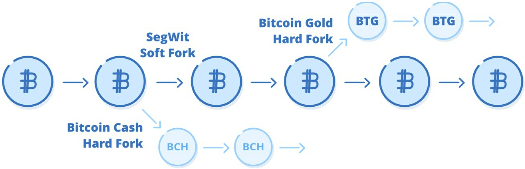
\includegraphics[width = 10cm]{imagens/Capitulo8/capitulo8-forks.png}
    \caption*{\textit{\small Moedas de um soft-fork podem ser enviada a nodes antigos. Um Hard-fork produz um novo retro incompatível UTXOs que não será aceito por nodes antigos}}
\end{figure}


Centenas de moedas semelhantes ao Bitcoin usam código semelhante, mas não compartilham o histórico de saldo da conta do Bitcoin (conjunto UTXO), como Litecoin ou Dogecoin.
Essas não são tipicamente consideradas divisões do Bitcoin embora dividam muito do mesmo código, pois elas não compartilham o histórico de saldo nas carteiras do bitcoin.

Um fork do Bitcoin não impacta sua oferta máxima de 21 milhões de Bitcoins. 
Imagine que você tem as reservas de ouro do mundo em um forte ultra seguro com segurança pesada.
Você construir uma pequena, mal montada cabana e chamar ela de forte lite, protegendo ela com um único segurança.
Podes pintar umas pedras de ouro e colocar elas dentro da cabana.
Quando anunciares ao mundo que você "forkou" o ouro e todos que detêm ouro podem deter a mesma quantia de pedras douradas em sua cabana.

Nos precisamos de muitos mineradores protegendo o bitcoin, tornando ele custoso a ataques de 51\%.  
Um fork do Bitcoin que só possui alguns mineradores, semelhantes a sua cabana mal protegida, é fácil de atacar. 
O código é provavelmente estruturalmente inseguro, construído por uma equipe de desenvolvedores sem experiencia, com péssima revisão por pares, igual a sua cabana. 
Moedas de forks não são aceitas por nodes porque quebram as regras do Bitcoin. 
Da mesma maneira que pessoas que tem testes químicos para o ouro não irão aceitar suas pedras douradas.
O custo de manufaturar as pedras e as moedas do fork é zero visto que deste elas de graça para todos os proprietários de ouro. 
Isso é limita o interesse do mercado em forks do Bitcoin.

Enquanto você considera as milhares de copias do Bitcoin que já foram criadas, e nenhuma os quais possui valor de mercado significativo, pense nesse paradoxo:
Criar forks do Bitcoin é gratuito e fácil. Porem, mudar as regras do Bitcoin ou criar Bitcoin novos é tudo menos fácil. 
A próxima vez que você ouvir alguém com conhecimento limitado sobre o bitcoin perguntar porque o Bitcoin é especial responda com isso.


%modificado
A natureza descentralizadas do ecossistema do Bitcoin cria uma forte preferencia ao modelo atual. 
Mudanças significativas precisam de meses ou anos de muito debates, construções de consenso e revisão por pares para ser implementado.
Isso é algo bom, e algo que almejamos de um sistema que visa ser a moeda do planeta.
Bitcoin é uma dança delicada entre milhares de participantes, todos agindo de forma egoísta e muitas vezes com necessidades concorrentes.
É um sistema anarquista de mercado verdadeiramente livre, sem ninguém em particular no comando.
\part{Passado, Presente e Futuro}
\label{ch:capitulo9}
\chapter*{Passado, Presente e Futuro}

Agora, munidos da compreensão da rede Bitcoin como um todo, podemos examinar alguns comportamentos interessantes que surgiram nos últimos dez anos do sistema.

\paragraph{ASICs e pools de mineração}
\paragraph{}

No início, Satoshi minerou os primeiros bitcoins usando a unidade de processamento central (CPU) do computador. Como a dificuldade inicial de mineração no sistema era baixa, era relativamente barato gerar essas moedas usando a CPU.

Com o tempo, as pessoas começaram a ajustar o software de mineração para torná-lo cada vez mais eficiente. Eventualmente, eles escreveram um software que começou a tirar proveito de processadores especializados chamados unidades de processamento gráfico (GPUs) que existem nas placas de vídeo e geralmente são usados para jogos.

Com as GPUs, a mineração tornou-se milhares de vezes mais eficiente do que a mineração usando a CPU. Nesse ponto, qualquer pessoa que minerava em uma CPU fornecia uma fração tão pequena da taxa de hash que rapidamente se tornou inútil, pois a dificuldade aumentou devido a todos os novos mineradores de GPU.

Conforme as GPUs assumiram o controle e as pessoas começaram a comprar toneladas de placas gráficas, a eficiência da mineração foi aprimorada ainda mais por meio da produção de ASICs (Application Specific Integrated Circuits, ou Circuitos Integrados Específicos de Aplicações em português). São chips de hardware de computador que são criados com um objetivo específico - a função bitcoin sha256 e nada mais. Sendo especializados neste algoritmo em particular, os ASICs foram capazes de ser milhares de vezes mais eficientes do que as GPUs para mineração e rapidamente tornaram as GPUs não lucrativas, assim como as GPUs fizeram com as CPUs. Em poucos anos, a nova geração de dispositivos ASIC coloca suas versões anteriores fora do mercado com grandes melhorias de eficiência.

Os primeiros mineradores da rede gastaram apenas alguns centavos de eletricidade para produzir seus bitcoins. À medida que o preço do bitcoin subia e mais e mais mineradores aderiam a rede, a dificuldade aumentava e ficava cada vez mais caro gerar bitcoins.

Um problema com a mineração de bitcoin é que ela não é determinística, como jogar um dado. Isso significa que você pode acabar gastando centenas de dólares em eletricidade e nunca encontrar um bloco válido.

Em 2010, uma inovação chamada pool de mineração (conhecida como Slushpool) surgiu para resolver o problema de mineradores consumindo energia sem receber recompensa. Um pool de mineração é um pool de risco compartilhado, semelhante ao funcionamento do seguro médico.

Todos os mineradores contribuem com a mineração, fazendo com que todos os participantes pareçam um grande mineirador. Se alguém na pool encontrar um bloco válido, a recompensa pelo bloco é dividida proporcionalmente entre todos os mineradores com base na taxa de hash com que contribuíram. Isso permite que até mesmo pequenas operações de mineração, como indivíduos, recebam recompensa pela pequena taxa de hash com que contribuem. Para fornecer este serviço de coordenação, o pool fica com uma parte das recompensas.
\newpage
Os pools de mineração causaram um efeito de centralização, os usuários migraram para pools maiores. O diagrama abaixo mostra a distribuição aproximada da mineração em janeiro de 2019.

\begin{figure}
  \centering
  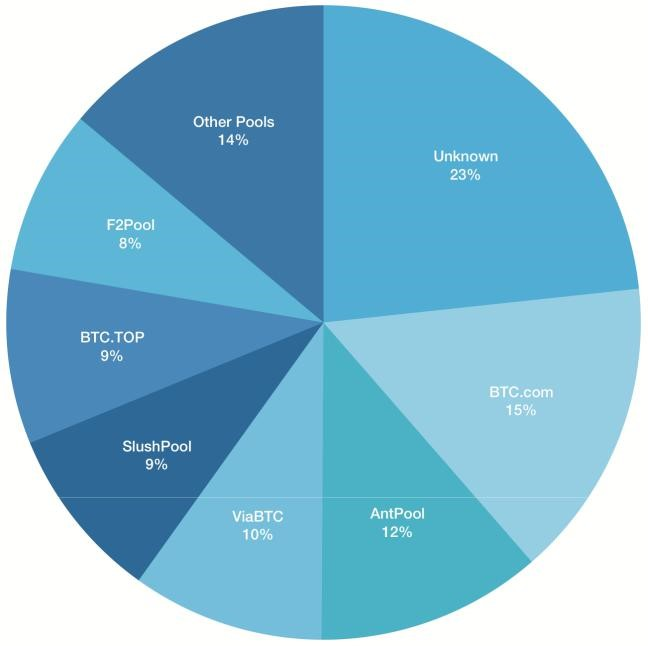
\includegraphics[width=7cm]{imagens/capitulo-9-pizza.jpg}
  \caption{Pools de mineração}
\end{figure}

\paragraph{Ataques de 51\%}
\paragraph{}

A centralização do pool de mineração leva à preocupação de que eles possam conspirar para 51\% atacar a rede. Se você olhar o gráfico acima, verá que as 5 principais pools, em conjunto, têm mais de 50\% da taxa de hash de mineração total.

Vamos examinar como esse ataque é realizado e quais perigos ele carrega.

Quando você possui pouco mais de 50\% da taxa de hash, pode dominar as gravações no livro-razão porque pode produzir uma cadeia mais longa do que a outra taxa de hash inferior a 50\% combinada ao longo do tempo. Lembre-se de que o Consenso de Nakamoto diz que os nodes devem aceitar a cadeia de Prova de Trabalho cumulativa mais longa que chegar até eles.

Aqui está um exemplo de como um ataque simples de 51\% é realizado:

\begin{enumerate}
\item Digamos que a rede como um todo esteja produzindo 1000 hashes/segundo;
\item Você compra um monte de hardware de mineração e eletricidade para produzir 2.000 hashes/segundo. Agora você tem 66\% da taxa total de hash (2000/3000);
\item Você começa a minerar uma cadeia que contém apenas blocos vazios;
\item Daqui a duas semanas, você transmitirá sua blockchain vazia. Como você está minerando aproximadamente duas vezes mais rápido que os mineradores honestos, sua cadeia será duas vezes mais longa focando na Prova de Trabalho cumulativa. A transmissão para todos os nodes existentes fará com que eles se reorganizem e percam as últimas duas semanas de história escrita na blockchain.
\end{enumerate}

Além de minerar blocos vazios, o que torna a blockchain inutilizável, você também pode realizar um ataque de gasto duplo:

\begin{enumerate}
\item Envie algum bitcoin para uma exchange;
\item Troque por USD e retire o USD;
\item Mais tarde, transmita na blockchain que você minerou secretamente e que não contém o envio para a exchange;
\item Você reescreveu a história e agora tem o bitcoin original e os dólares;
\end{enumerate}

Na prática, com a taxa de hash do Bitcoin hoje (lembre-se, ele está usando a mesma quantidade de energia de um país de porte médio), adquirir hardware e eletricidade suficientes para realizar tal ataque é extremamente caro. Também é muito difícil escapar impune com um ataque de gasto duplo dessa proporção sem deixar pegadas que poderiam ser usadas para descobrir quem você é. Afinal, você estaria consumindo a energia de um país de porte médio e comprando milhões de dólares em hardware e enviando milhões de dólares para a exchange para fazer todo este processo.

Manter esse tipo de ataque por qualquer período de tempo razoável é inviável, e se alguma entidade mal-intencionada com financiamento ilimitado decidisse fazer isso e fosse capaz de sustentar esse ataque além do nível de um incômodo, a rede poderia se adaptar alterando a sua função de prova de trabalho (usando alguma coisa diferente do sha256), que tornaria todos os ASICs de hardware usados pelo invasor completamente inúteis. Essa, no entanto, é a opção nuclear, pois também tiraria do mercado imediatamente todos os mineradores honestos. No entanto, a rede sobreviveria e surgiria das cinzas, como a Fênix.

Além da inviabilidade do ataque, ter a maioria da taxa de hash não dá direito a ser dono da rede:

\begin{enumerate}
\item Você não pode criar moedas do nada. Isso viola a regra de consenso de recompensa de blocos, sendo eles rejeitados, mesmo se tivessem Prova de Trabalho suficiente;
\item Você não pode gastar moedas que não são suas. Você não seria capaz de fornecer uma assinatura digital válida, o que viola as regras;
\item Você não pode acelerar o cronograma de emissão de Bitcoin. A dificuldade seria ajustada a cada 2016 blocos como sempre faz.
\end{enumerate}

Assim, os nodes que aceitam Bitcoin como pagamento manteriam a rede honesta mesmo em face de uma maioria desonesta de mineradores. Além disso, não devemos presumir que, apenas porque um pool de mineração tem uma porcentagem específica de taxa de hash, eles possuem o hardware. Na verdade, a maioria das pools de mineração é composta por milhares de mineradores individuais. Se o pool de mineração começar a se comportar mal, esses mineradores teriam um incentivo para sair do pool porque gostariam de proteger o valor econômico do Bitcoin, que estão minerando presumivelmente para ganhar dinheiro e não para ter prejuízos!

Na verdade, há um precedente histórico para mineradores individuais deixarem uma pool que se tornou muito poderosa: em 2014, a Ghash.io tinha quase metade do poder de mineração total. Os mineiros viram que ele estava se tornando muito centralizada e partiram para outras pools de maneira voluntaria.

Embora pools de mineração relativamente centralizadas sejam a realidade atual, há melhorias constantes na tecnologia de mineração, incluindo uma proposta chamada BetterHash, que permite que os mineradores individuais tenham mais controle sobre o que estão minerando e reduza a dependência da coordenação das pools.

\paragraph{Hard Forks e Soft Forks}
\paragraph{}

Deixamos o tópico mais complexo do Bitcoin para o final.

Esperamos que agora você tenha um bom controle sobre como o software Bitcoin impõe as regras que as pessoas concordaram e como as pessoas podem decidir qual software executar para aplicar as regras em que acreditam.

Também falamos que os mineradores decidem as regras que seguirão ao produzir blocos e que devem minerar o tipo de blocos que os usuários desejam, ou arriscar que seus blocos não sejam aceitos e, assim, perder a recompensa da mineração.

Finalmente, sabemos que o software do Bitcoin aceitará a mais longa cadeia de prova cumulativa de trabalho como sendo a blockchain válida, e que forks (ou bifurcações em português), às vezes, ocorrem naturalmente devido à mineração dos mineradores usando as cadeias desatualizadas.

Agora vamos falar sobre forks intencionais. Um fork intencional é quando alguns usuários e/ou mineradores decidem que não concordam com as regras atuais do Bitcoin e que precisam mudar as regras. Existem dois tipos de forks, que mudam as regras que foram definidas anteriormente: soft forks, que são compatíveis com versões anteriores, e hard forks, que não são compatíveis com versões anteriores. Vamos ver como isso ocorre na teoria e, em seguida, ver alguns exemplos históricos.

\paragraph{Soft Forks}
\paragraph{}

Um soft fork é uma mudança compatível com as regras de consenso do Bitcoin. O que isso significa? Isso significa que se você executar um node antigo que não foi atualizado para as novas regras, ele ainda verá os blocos produzidos sob as novas regras como válidos. Para um node atualizado com o novo software soft fork, todos os blocos que eram anteriormente inválidos permanecem inválidos, mas alguns blocos válidos agora são considerados inválidos. Vejamos um exemplo para deixar claro:

Em 12 de setembro de 2010, uma nova regra foi introduzida no software: Os blocos devem ter no máximo 1 MB de tamanho. Esta regra foi introduzida para resolver problemas de spam na blockchain. Antes dessa regra, todos os blocos de qualquer tamanho eram válidos. Com a nova regra, apenas blocos menores eram válidos. Se você estava executando um node antigo e não o atualizou, os blocos menores ainda eram válidos de acordo com suas regras, então você não foi afetado.

Um soft-fork é uma maneira de atualizar o sistema sem interrupções porque permite que os operadores dos nodes atualizem para o novo software lentamente ao longo do tempo, de forma voluntária. Se eles não fizerem a atualização, eles ainda serão capazes de processar todos os blocos que chegam como sempre fizeram. Apenas os  mineradores que produzem os blocos precisam se atualizar para começar a produzir blocos usando as novas regras. Depois que os mineradores atualizaram para o novo fork de 1 MB, todos os blocos daquele ponto em diante tinham no máximo 1 MB de tamanho. Os usuários que executam versões antigas do software não precisavam saber disso.


\paragraph{Hard Forks}
\paragraph{}

Um hard fork é o oposto de um soft fork. No caso de um hard fork, uma alteração não compatível com versões anteriores é introduzida na qual os blocos que eram originalmente inválidos agora são considerados válidos. No caso de um hard fork, os nodes antigos que não foram atualizados não serão capazes de processar os blocos produzidos sob as novas regras. Assim, eles ficarão presos na blockchain antiga, a menos que façam a atualização. Um exemplo de hard fork seria aquele que alterasse o tamanho do bloco de 1 MB para algo maior, pois os blocos seriam inválidos de acordo com as regras antigas.

A maioria dos hard forks com concordância quase unânime de todos os nodes da rede não causaria problemas. Cada node seria atualizado imediatamente para as novas regras. Se alguns retardatários fossem deixados para trás, eles não obteriam novas atualizações de bloco e consequentemente notariam que seu software parou de funcionar e seriam forçados a atualizá-los.

Na prática, os hard forks nunca são feitos de maneira suave. Em um sistema anárquico verdadeiramente descentralizado, você não pode coagir todos a mudarem para as novas regras. Em agosto de 2017, algumas pessoas que não estavam felizes com o progresso da rede Bitcoin em relação a pagamentos baratos decidiram que queriam fazer um fork para criar uma rede com blocos maiores. Como o Bitcoin tinha uma regra sobre os blocos não ultrapassarem 1 MB (devido a um soft fork ocorrido em 2010), essas pessoas queriam criar uma nova cadeia com blocos maiores. Este fork ficou conhecido como Bitcoin Cash.

Um hard fork fora do consenso como Bitcoin Cash, que não é seguido por todos os mineradores e nodes, cria uma nova blockchain que compartilha alguma história com a blockchain original, mas a partir do ponto de divisão em diante, as moedas criadas no fork não são mais Bitcoin, pois não são aceitas por nenhum node da rede Bitcoin.

O assunto o que “é” ou “não é” Bitcoin foi calorosamente debatido no ano seguinte ao fork do Bitcoin Cash. Houve algumas pessoas em favor do Bitcoin Cash que propuseram uma narrativa de que o Bitcoin deve ser definido pelo que está escrito no white paper original, escrito por Satoshi há dez anos, escolhendo a dedo as palavras específicas no documento para provar seu ponto. Mas um sistema baseado em consenso não funciona com base em argumentos feitos nas redes sociais. Funciona por pessoas que optam por executar um software específico para fazer cumprir regras específicas.

No caso deste fork, as pessoas que executam a grande maioria dos nodes economicamente significativos - ou seja, carteiras, exchanges e comerciantes não queriam trocar seu software por algo suportado por uma equipe de desenvolvimento muito menor e menos experiente e em uma quantidade muito menor de hash que sinalizou que eles queriam mudar para essas regras. Nem as pessoas achavam que tal “atualização” valesse a pena quando comparado a possibilidade de interrupção do ecossistema. O problema com os hard forks é que eles só funcionam quando todos aceitam a troca. Se houver retardatários, duas moedas são criadas. Assim, o Bitcoin permaneceu como sendo o Bitcoin e o Bitcoin Cash tornou-se uma moeda separada.

Hoje, existem dezenas de outros forks de Bitcoin, como Bitcoin Gold, Bitcoin Diamond e Bitcoin Private, com um pequeno hash protegendo-os, baixo suporte ao desenvolvedor e atividade econômica quase inexistente. Muitos são golpes ou projetos de pesquisa mal elaborados. Centenas de moedas semelhantes ao Bitcoin usam código semelhante, mas não compartilham o histórico de saldo da conta do Bitcoin (conjunto UTXO), como Litecoin ou Dogecoin.

\paragraph{O Livre Mercado}
\paragraph{}

Mencionamos brevemente as taxas de transação no Capítulo 5 ao discutir a mineração, mas elas merecem sua própria seção. Uma vez que a programação de emissão de Bitcoin consiste em halvings acontecendo a cada quatro anos, até que a Recompensa de Bloco seja totalmente eliminada e o Bitcoin entre em um estado de cunhagem zero até o fim dos tempos, ainda precisamos de uma forma de incentivar os mineradores a continuarem protegendo a rede .

As taxas são determinadas por um sistema de livre mercado, no qual os usuários pagam por espaço escasso em um bloco. Os usuários que enviam transações indicam quanta taxa estão dispostos a pagar aos mineradores, e eles podem ou não incluir as transações que são informadas, dependendo do quanto irão ganhar. Quando há poucas transações esperando para entrar no próximo bloco, as taxas tendem a ser muito baixas, pois não há competição. À medida que o espaço do bloco é preenchido, os usuários estão dispostos a pagar taxas mais altas para que suas transações sejam confirmadas rapidamente (no próximo bloco). Aqueles que não querem pagar, podem sempre definir taxas baixas e esperar mais para serem minerados em um momento com baixa demanda, quando o espaço do bloco estiver mais disponível.

Ao contrário dos sistemas financeiros tradicionais, onde as taxas tendem a se basear em uma porcentagem do valor que está sendo transferido, no Bitcoin o valor transferido não tem relação com as taxas. Tornamos as taxas proporcionais ao recurso escasso que consomem: espaço em bloco. Portanto, as taxas são medidas em satoshis por byte (bytes são 8 bits, basicamente apenas uma medida de quantos dados há em sua transação). Assim, uma transação que envia um milhão de bitcoins de um endereço para outro pode ser mais barata do que uma que consolida 1 bitcoin espalhado por 10 contas, porque o último requer mais espaço de bloco.

No passado, houve períodos em que o Bitcoin tinha uma demanda muito alta, como o que aconteceu no final de 2017, onde as taxas se tornaram extremamente altas. Desde então, alguns novos recursos foram implementados para reduzir a pressão sobre as taxas na rede.

Um deles é chamado de Segregated Witness (ou Testemunha Segregada), que reorganizou como os dados do bloco são representados separando as assinaturas digitais dos dados da transação, criando mais espaço para esses dados. As transações que tiram proveito desta atualização podem usar mais do que o 1 MB original do espaço do bloco por meio de alguns truques inteligentes que estão além do escopo deste livro.

O outro alívio para as taxas veio através do batching: As exchanges e outros participantes de alto volume no ecossistema começaram a combinar transações de bitcoin para vários usuários em uma transação. Ao contrário de um pagamento tradicional em seu banco ou PayPal que é feito de uma pessoa para outra, uma transação de Bitcoin pode combinar um grande número de entradas e produzir um grande número de saídas. Assim, uma exchange que precisa enviar bitcoin para saque para 100 pessoas pode fazê-lo em uma única transação. Este é um uso muito mais eficiente do espaço do bloco, transformando o que é ostensivamente apenas um punhado de transações de bitcoin por segundo em milhares de pagamentos por segundo.

A Segregated Witness e o batching já fizeram um trabalho muito bom na redução da demanda por espaço em bloco. Outras melhorias estão em andamento para tornar o uso do espaço do bloco mais eficiente. No entanto, chegará um momento em que as taxas de Bitcoin ficarão altas novamente, à medida que os blocos ficarem cada vez mais cheios devido à demanda.
 
\paragraph{Desenvolvimentos futuros no Bitcoin}
\paragraph{}

Neste ponto, já passamos por toda a questão de \textit{inventar o Bitcoin} e cobrimos como a rede evoluiu ao longo do tempo. Agora olhamos para o futuro e cobrimos algumas das melhorias de curto prazo que virão para o Bitcoin.

Ao contrário de uma moeda tradicional, que é algo que é impresso e usado, o Bitcoin é uma camada de dinheiro programável sobre a qual podemos construir muitos serviços. Este é um conceito totalmente novo e estamos apenas começando a ter conhecimento do que é possível ser feito.

\paragraph{Lightning Network}
\paragraph{}

Como discutimos acima, o Bitcoin teve problemas com taxas altas à medida que o espaço em bloco se tornou cada vez mais procurado. Hoje, o Bitcoin é capaz de apenas cerca de 3 a 7 transações por segundo com base no número de transações que cabem em um bloco. Lembre-se que cada transação pode, na verdade, ser um pagamento para centenas de pessoas por lote. Ainda assim, não tem a capacidade suficiente para se tornar uma rede global de pagamentos.

Uma solução ingênua pode ser aumentar o tamanho do bloco, e de fato várias moedas concorrentes, incluindo o Bitcoin Cash, tentaram essa abordagem. O Bitcoin não segue esse caminho porque aumentar o tamanho do bloco impactaria negativamente as características de descentralização, como o número de nodes e a dispersão geográfica. Mesmo que um aumento no tamanho do bloco fosse possível devido a melhorias no hardware, há também o problema de que a natureza descentralizada do Bitcoin significa que um hard fork que tenta mudar o tamanho do bloco causaria muitos problemas, e provavelmente ocorreria outra divisão da blockchain, criando assim, uma moeda diferente.

Um aumento no tamanho do bloco também não resolveria o problema de tornar o Bitcoin adequado como um sistema de pagamento mundial - ele simplesmente não seria tão escalável. É aqui que entra a Lightning Network: Outro protocolo e conjunto de implementações de software que criam transações offchain de Bitcoins.
 
The Lightning Network pode ser o assunto de todo um livro, mas vamos discuti-la brevemente.

A ideia da Lightning é que nem todas as transações precisam ser registradas na blockchain. Por exemplo, se você e eu estamos em um bar comprando bebidas, podemos abrir uma conta no bar e resolver no final da noite. Realmente não faz sentido cobrarmos de nosso cartão de crédito por cada bebida, pois é uma perda de tempo. Com o Bitcoin, usar a energia equivalente à de um país inteiro ao confirmar a compra de um café ou cerveja e ter essa compra registrada o tempo todo em milhares de computadores em todo o mundo não é escalonável nem particularmente bom para a privacidade.

A Lightning Network, se for bem-sucedida, melhorará muitas das desvantagens do Bitcoin:

\begin{enumerate}
\item Transferência de transações virtualmente ilimitada. Centenas de milhares de micro transações poderiam ser realizadas usando a blockchain Bitcoin uma vez, como liquidação final;
\item Confirmações instantâneas; não há necessidade de esperar que os blocos sejam minerados;
\item Taxas de transação de menos de um centavo adequadas para micro pagamentos, como pagar um centavo para ler um blog;
\item Maior privacidade. Apenas as partes que participam da transação precisam saber sobre ela, ao contrário de uma transação em rede que é transmitida para o mundo inteiro.
\end{enumerate}

A Lightning usa o conceito de canais de pagamento, que são transações reais de Bitcoin na blockchain que bloqueiam uma certa quantidade de Bitcoin e o tornam disponível na Lightning Network para transferência instantânea e quase gratuita. A Lightning Network está nos estágios iniciais, mas já se mostra promissora. Você pode verificar o site \textit{\url{https://yalls.org/}} que usa micro pagamentos baseados na Lightning para disponibilizar a leitura de artigos.

\paragraph{Bitcoin no Espaço}
\paragraph{}

O Bitcoin faz um excelente trabalho de ser resistente à censura, pois é resistente ao confisco (você pode carregá-lo em sua cabeça) e resistente à censura de transferência, uma vez que requer apenas um minerador honesto na rede para garantir suas transações (e você pode minerar você mesmo).

No entanto, sendo o Bitcoin transmitido pela Internet, é suscetível de censura em nível de rede. Os regimes autoritários que querem reprimir a atividade podem tentar bloquear o tráfego de Bitcoin que entra e sai de seu país.

O Blockstream Satellite é o primeiro esforço para contornar a censura de rede em nível estadual, bem como alcançar áreas remotas que podem não ter conexões com a Internet. Este satélite permite que qualquer pessoa com uma antena parabólica e equipamento relativamente barato conecte e baixe a blockchain do Bitcoin, com comunicação bidirecional em breve. Agora também existem esforços como o TxTenna para construir redes fora da grade elétrica. Quando acoplado a uma conexão via satélite, esse tipo de configuração seria quase imparável\footnote{Nota do tradutor: Atualmente um grupo de brasileiros usou ondas de rádio para colocar uma transação na rede usando a Lua como ponto de reflexo. Veja mais em \url{https://livecoins.com.br/brasileiros-enviam-bitcoin-a-lua-na-frente-de-elon-musk/}}.
\part{O Que Vem Depois?}
\label{ch:capitulo10}
\chapter*{O Que Vem Depois?}

Então é isso. Você passou pelo exercício de \textit{Inventar o Bitcoin} e, com sorte, emergiu do outro lado do espelho, pronto para explorar mais sobre o assunto. Onde você conseguirá mais informações? Aqui estão alguns recursos para ajudá-lo a explorar a toca do coelho:

Para saber mais sobre a economia por trás do Bitcoin:

\begin{itemize}
\item \href{https://amzn.to/2V1vQ62}{O padrão Bitcoin} do Saifedean Ammous;
\item \href{https://amzn.to/3jwpiG7}{Criptoativos} do Chris Burniske e Jack;
\item \href{https://tinyurl.com/bzrkbb5u}{Pesquisar no Google: Economia Austríaca};
\item \href{https://tinyurl.com/3yn8amt3}{Bitcoin Investment Theses} do Pierre Rochard;
\item \href{https://tinyurl.com/f8e4wn5h}{The Bullish Case for Bitcoin} do Vijay Boyapati.
\end{itemize}

Para se aprofundar na ciência da computação:

\begin{itemize}
\item O \href{https://bitcoin.org/bitcoin.pdf}{whitepaper do Bitcoin} escrito por Satoshi Nakamoto;
\item \href{https://amzn.to/3gOqaUH}{Mastering Bitcoin} do Andreas Antonopulous;
\item O \href{https://programmingbitcoin.com/#programming-blockchain}{Seminário} do Jimmy Song;
\item \href{https://programmingblockchain.gitbook.io/programmingblockchain/}{Programming Blockchain} também do Jimmy Song.
\end{itemize}

Para se aprofundar na história e filosofia do Bitcoin:

\begin{itemize}
\item \href{https://tinyurl.com/Planting-Bitcoin}{Planting Bitcoin} por Dan Held;
\item \href{https://tinyurl.com/mzy6jkz4}{Bitcoin Governance} do Pierre Richard;
\item \href{https://tinyurl.com/y8vueb88}{Bitcoin Past and Future} do Murad Mahmudov;
\item Todos os vídeos feitos por Andreas Antonopulous, especialmente \href{https://www.youtube.com/user/aantonop}{Currency Wars e The Monument of Immutability}.
\end{itemize}

Uma grande parte do ecossistema Bitcoin vive no Twitter. Deixarei aqui um punhado de pessoas, sem uma ordem específica, que seria interessante seguir. Comece nesta lista e vá diversificando conforme for encontrando novas mentes que caíram na toca do coelho:

\begin{itemize}
\item \href{https://twitter.com/lopp}{@lopp}
\item \href{https://twitter.com/pwuille}{@pwuille}
\item \href{https://twitter.com/adam3us}{@adam3us}
\item \href{https://twitter.com/danheld}{@danheld}
\item \href{https://twitter.com/TraceMayer}{@TraceMayer}
\item \href{https://twitter.com/pierre_rochard}{@pierre\_rochard}
\item \href{https://twitter.com/bitstein}{@bitstein}
\item \href{https://twitter.com/Melt_Dem}{@Melt\_Dem}
\item \href{https://twitter.com/theonevortex}{@theonevortex}
\item \href{https://twitter.com/WhatBitcoinDid}{@WhatBitcoinDid}
\item \href{https://twitter.com/stephanlivera}{@stephanlivera}
\item \href{https://twitter.com/TheBlock__}{@TheBlock\_\_}
\item \href{https://twitter.com/TheLTBNetwork}{@TheLTBNetwork}
\item \href{https://twitter.com/real_vijay}{@real\_vijay}
\item \href{https://twitter.com/jimmysong}{@jimmysong}
\item \href{https://twitter.com/Excellion}{@Excellion}
\item \href{https://twitter.com/starkness}{@starkness}
\item \href{https://twitter.com/roasbeef}{@roasbeef}
\item \href{https://twitter.com/saifedean}{@saifedean}
\item \href{https://twitter.com/giacomozucco}{@giacomozucco}
\item \href{https://twitter.com/Snyke}{@Snyke}
\item \href{https://twitter.com/aantonop}{@aantonop}
\item \href{https://twitter.com/MustStopMurad}{@MustStopMurad}
\item \href{https://twitter.com/peterktodd}{@peterktodd}
\item \href{https://twitter.com/skwp}{@skwp} (Autor do livro)
\item \href{https://twitter.com/KoreaComK}{@KoreaComK} (Tradutor do livro)
\end{itemize}

Você pode encontrar mais textos do autor do livro em\newline \url{https://yanpritzker.com}. Vejo você do outro lado.

\cleardoublepage

\chapter*{Agradecimentos}
\label{ch:agracedimentos}

Obrigado às diversas pessoas que me deram feedback durante os primeiros rascunhos deste livro. Em particular: Joe Levering, Phil Geiger, Yury Pritzker, Jonathan Wheeler e Walter Rosenberg.

Obrigado ao Jimmy Song por seu seminário de programação na Blockchain, que me deu o chute necessário que  precisava para montar este texto.
\chapter*{Sobre o Autor}
\label{ch:sobre o autor}

Yan Pritzker é desenvolvedor e empreendedor em startups há 20 anos. Mais recentemente, ele foi o CTO cofundador da \href{https://reverb.com/}{Reverb.com}, onde administrou a tecnologia e a infraestrutura durante o período de 2012 a 2018. Hoje ele está focado em educação e consultoria em Bitcoin para startups no estágio inicial.

Yan escreve sobre Bitcoin e tópicos relacionados em \href{https://yanpritzker.com/}{yanpritzker.com}.

Você também pode segui-lo no Twitter: \href{https://twitter.com/skwp}{@skwp}.

\end{document}
